%!TEX root = ../dissertation.tex
\begin{savequote}[75mm]
Madness and genius are separated only by degrees of success. 
%\qauthor{Tony}
\end{savequote}

\chapter{Result}
\paragraph{}
The signal regions in data was blinded to reduce the bias in selection optimization.
After approval within the ATLAS analysis group, the signal regions were unblinded in July, 2017.
The unblinded boosted signal region results are shown in section~\ref{sec:res-boostedsr}.
The resolved signal region results are shown in section~\ref{sec:res-resolvedsr}.
The boosted analysis observed limits for \Grav~ and scalar $H$ are shown in section~\ref{sec:observedlimits}.
The combined boosted and resolved limits are shown in section~\ref{sec:combinedlimits}.

\section{Boosted signal region}
\label{sec:res-boostedsr}
\paragraph{}
The unblinded signal region yields are summarized in Table ~\ref{tab:sr-summary}. 
The unscaled $2bs$/$3b$/$4b$s \mtwoJ~ distributions are shown in Figures~\ref{fig:boosted-2b-signal-l}, \ref{fig:boosted-3b-signal-l}, \ref{fig:boosted-4b-signal-l}. 
No significant excess in number of events or in the dijet mass distribution is observed.
The scaled \mtwoJ~ distributions are shown in Figures~\ref{fig:boosted-2b-signal-pole}, \ref{fig:boosted-3b-signal-pole}, \ref{fig:boosted-4b-signal-pole}. 
Again, no significant excess in the scaled \mtwoJ~ distribution is observed.
No events are observed with \mtwoJ~ or scaled \mtwoJ~ above $4$ \TeV.
The other kinematic distributions in the signal region are shown in Appendix~\ref{AppendixSR}.

\begin{table}[htb!]
\scriptsize
\begin{center}
\caption{Unblinded signal region predictions and results. All systematic uncertainties are included for backgrounds. The Poisson uncertainty in data is shown for comparison.}
\begin{footnotesize} 
\begin{tabular}{c|c|c|c} 
Sample & FourTag & ThreeTag & TwoTag split \\ 
\hline\hline 
qcd & 32.92 $\pm$ 7.07 & 702.16 $\pm$ 63.12 & 3393.81 $\pm$ 148.78\\ 
ttbar & 1.68 $\pm$ 1.43 & 79.41 $\pm$ 33.12 & 859.03 $\pm$ 107.86\\ 
totalbkg & 34.6 $\pm$ 6.28 & 781.56 $\pm$ 52.42 & 4252.83 $\pm$ 125.73\\ 
\hline 
Data & 31.0 $\pm$ 5.57 & 801.0 $\pm$ 28.3 & 4376.0 $\pm$ 66.15\\ 
\hline\hline 
\end{tabular} 
\end{footnotesize} 
\newline 

\label{tab:sr-summary}
\end{center}
\end{table}

%%%%%%%%%%%%%%%%%%%%%%%%%%%plots%%%%%%%%%%%%%
\begin{figure*}[htb!]
\begin{center}
    \captionsetup{justification=centering}
    \begin{subfigure}[b]{0.45\textwidth}
        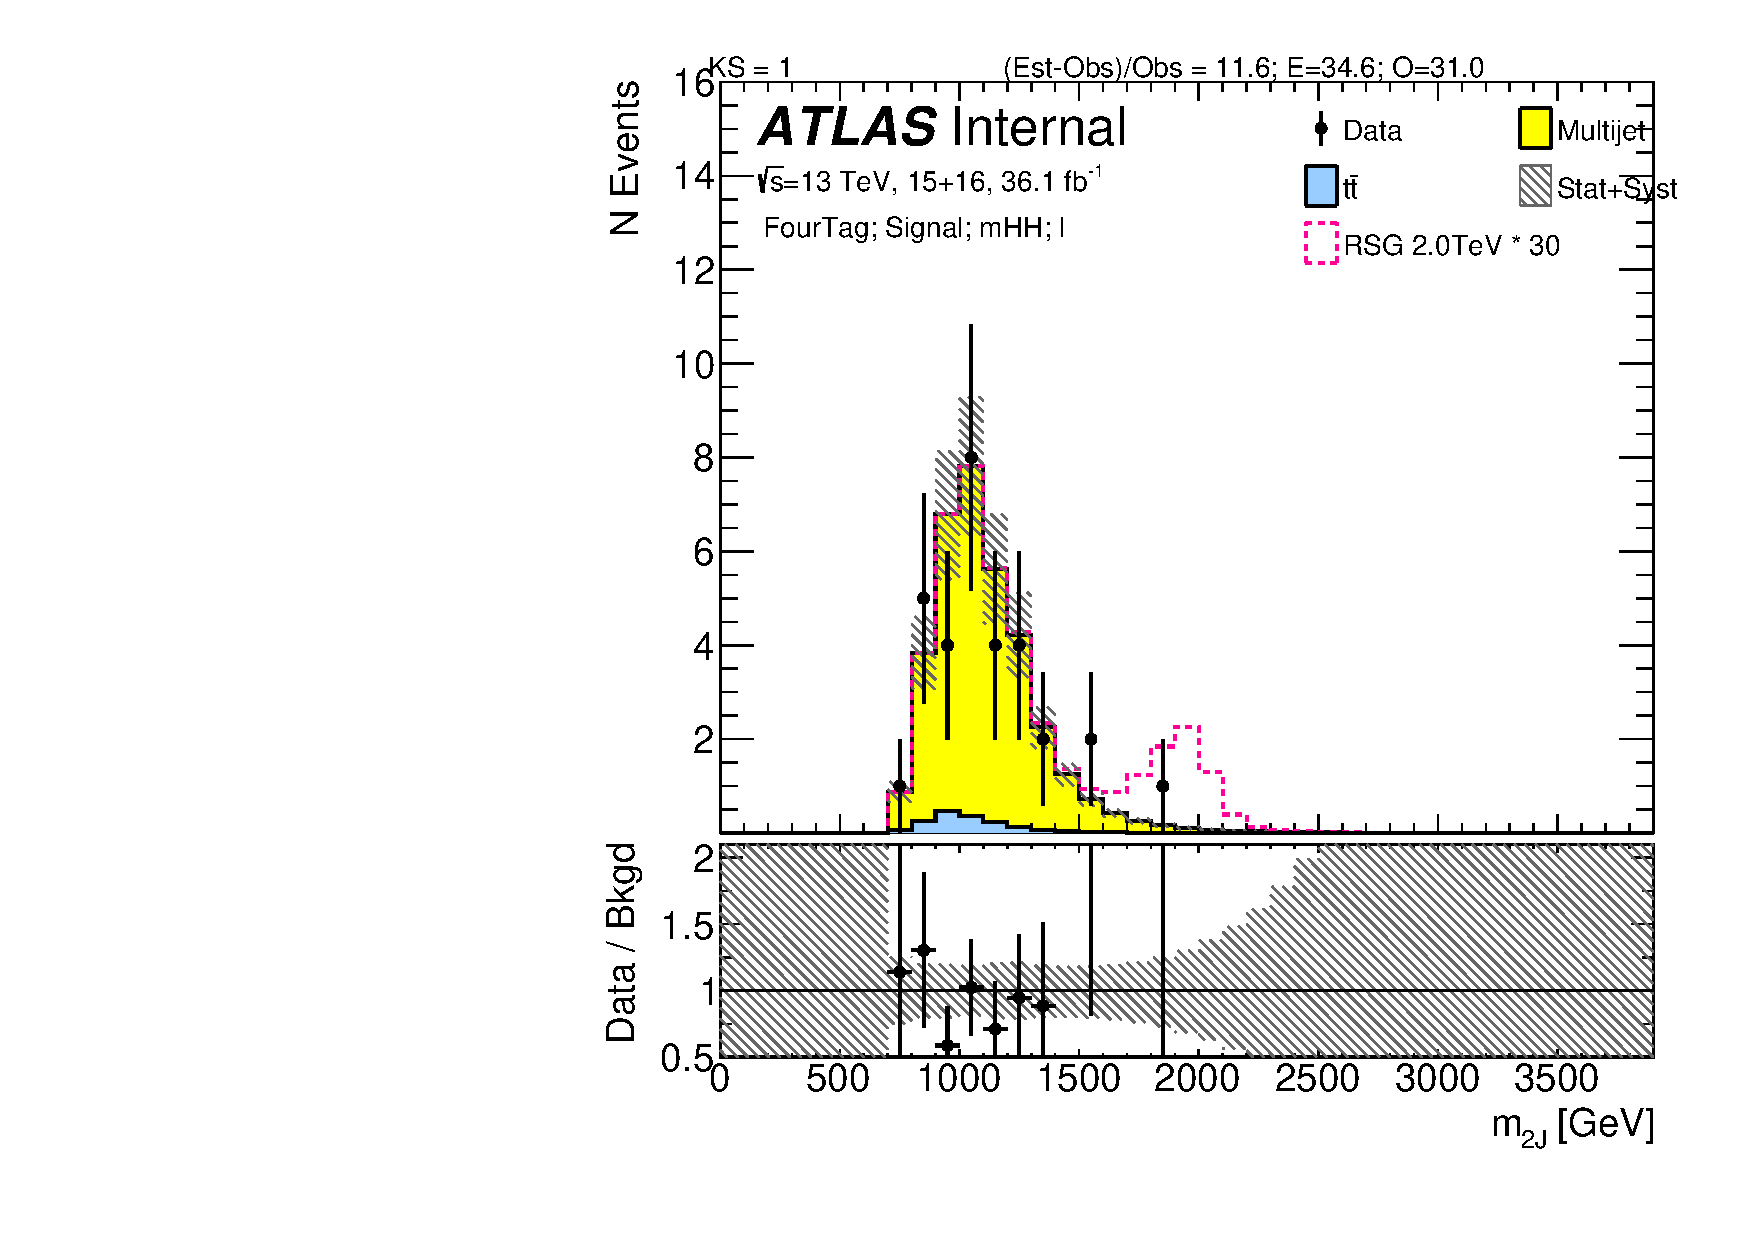
\includegraphics[width=\textwidth,angle=-90]{figures/boosted/Signal_Syst/Moriond_bkg_9_FourTag_Signal_mHH_l.pdf}
        \caption{Linear-$y$}
        \label{fig:boosted-4b-signal-lin}
    \end{subfigure}
    \quad
    \begin{subfigure}[b]{0.45\textwidth}
        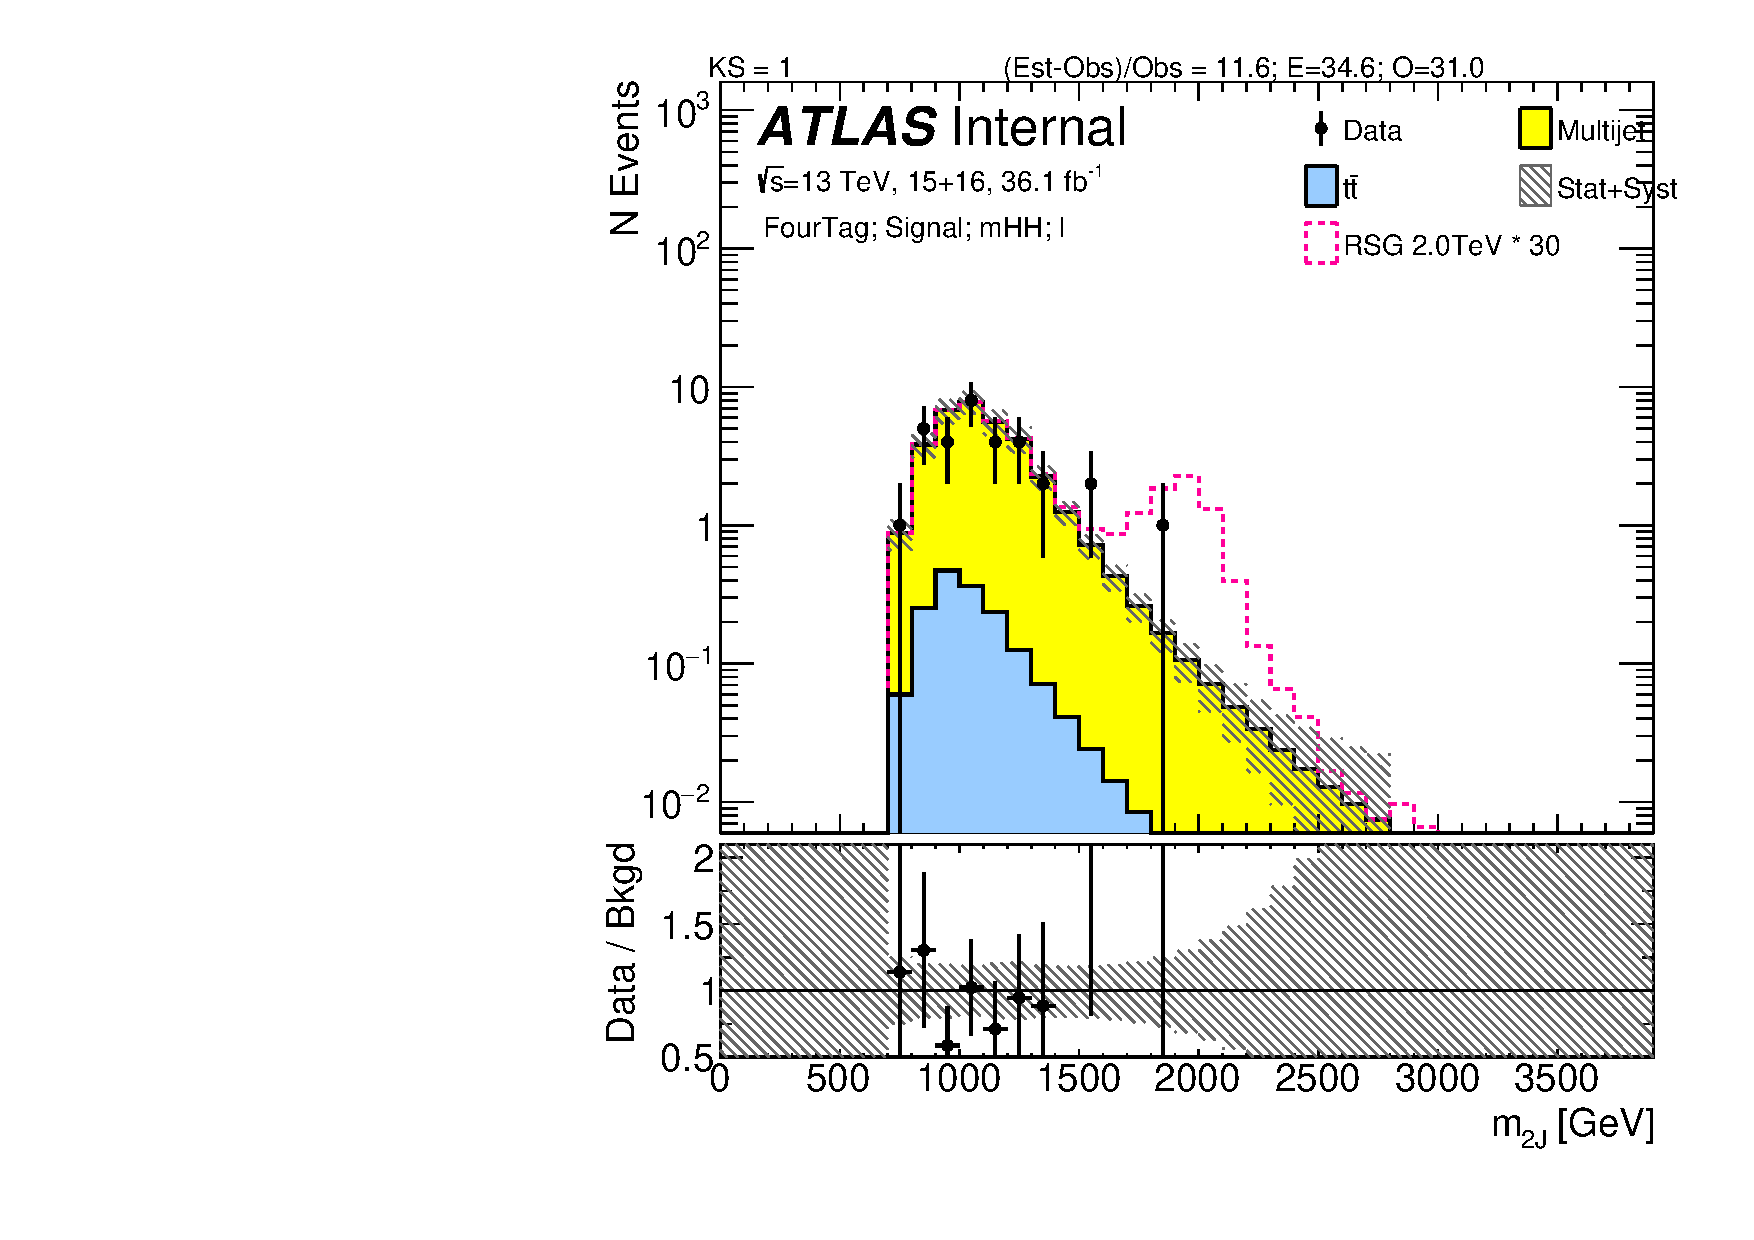
\includegraphics[width=\textwidth,angle=-90]{figures/boosted/Signal_Syst/Moriond_bkg_9_FourTag_Signal_mHH_l_1.pdf}
        \caption{Log-$y$}
        \label{fig:boosted-4b-signal-log}
    \end{subfigure}
  \caption{Unscaled \mtwoJ~ distribution in the $4b$ signal region after unblinding.}
  \label{fig:boosted-4b-signal-l}
\end{center}
\end{figure*}


\begin{figure*}[htb!]
\begin{center}
    \captionsetup{justification=centering}
    \begin{subfigure}[b]{0.45\textwidth}
        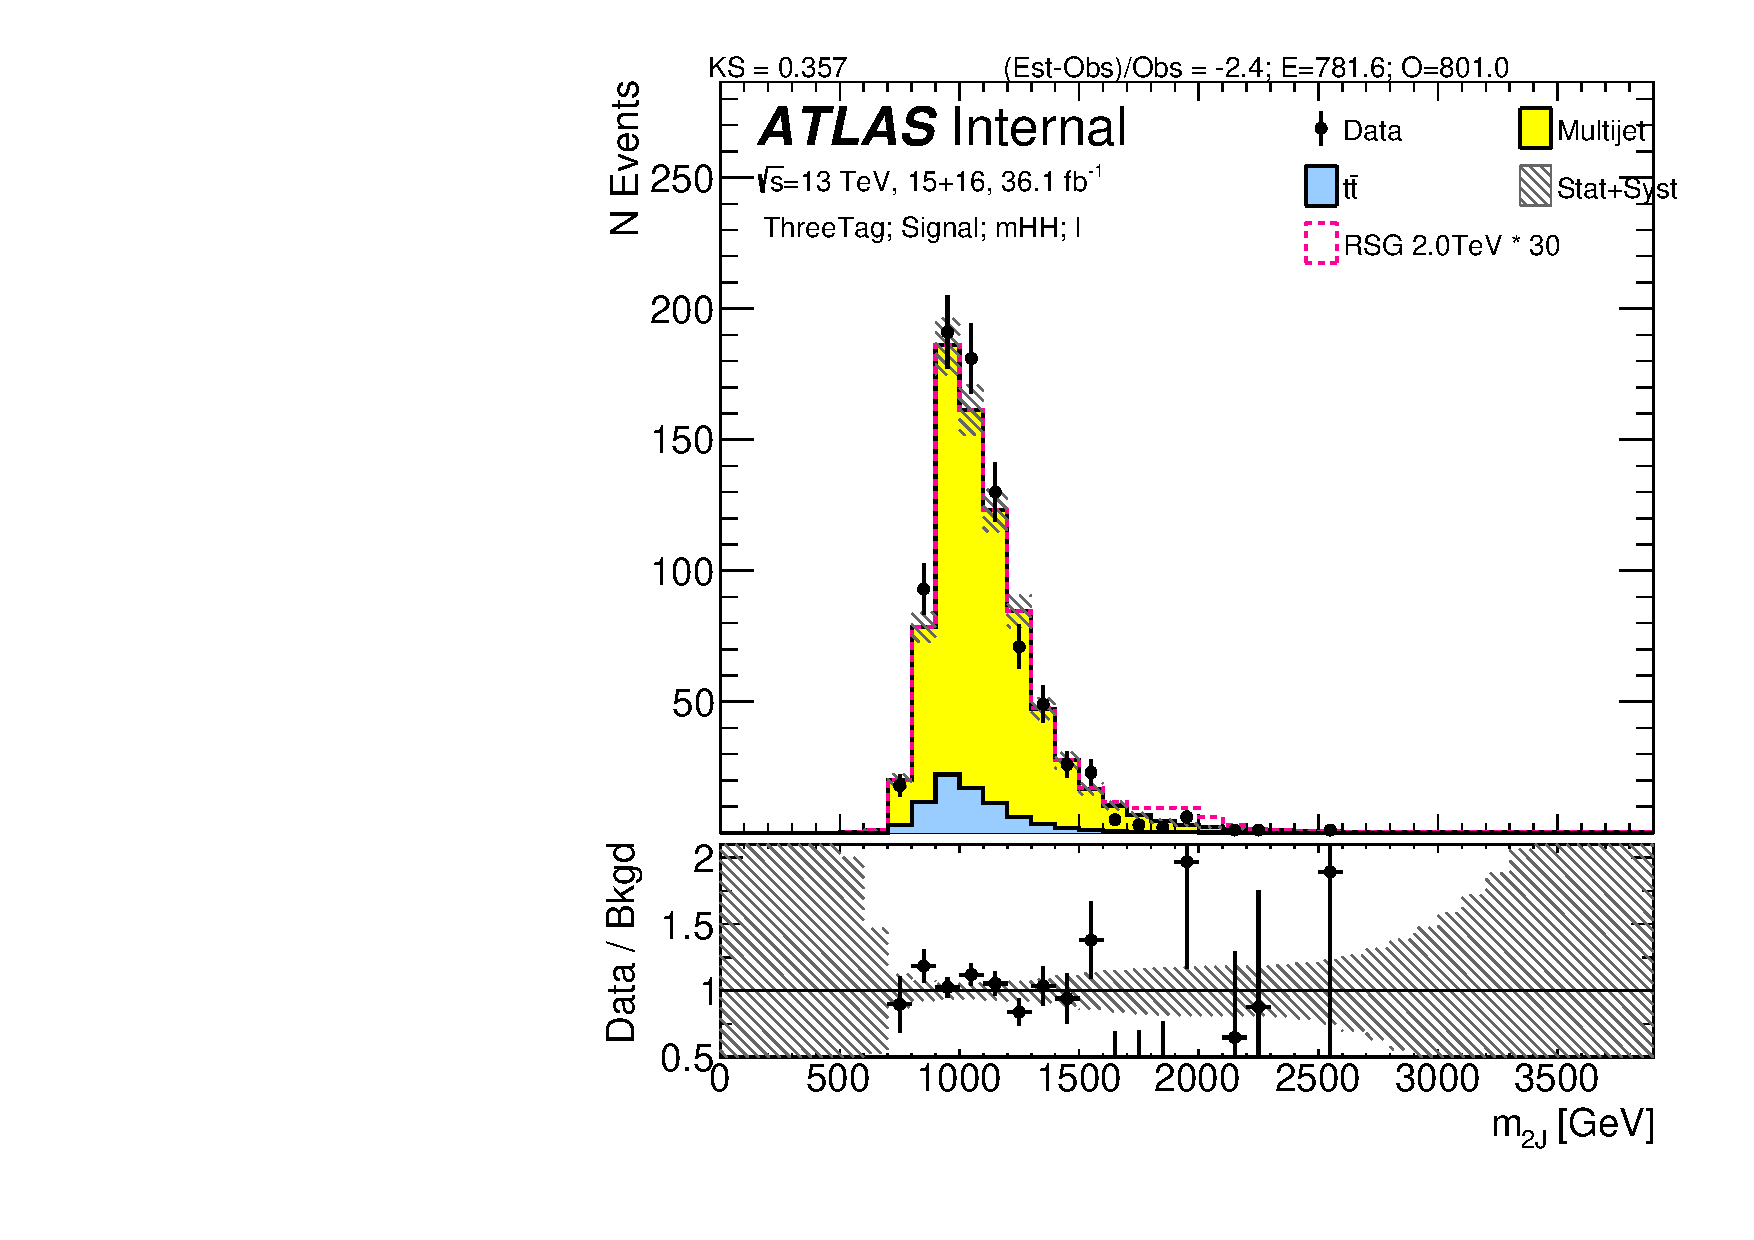
\includegraphics[width=\textwidth,angle=-90]{figures/boosted/Signal_Syst/Moriond_bkg_9_ThreeTag_Signal_mHH_l.pdf}
        \caption{Linear-$y$}
        \label{fig:boosted-3b-signal-lin}
    \end{subfigure}
    \quad
    \begin{subfigure}[b]{0.45\textwidth}
        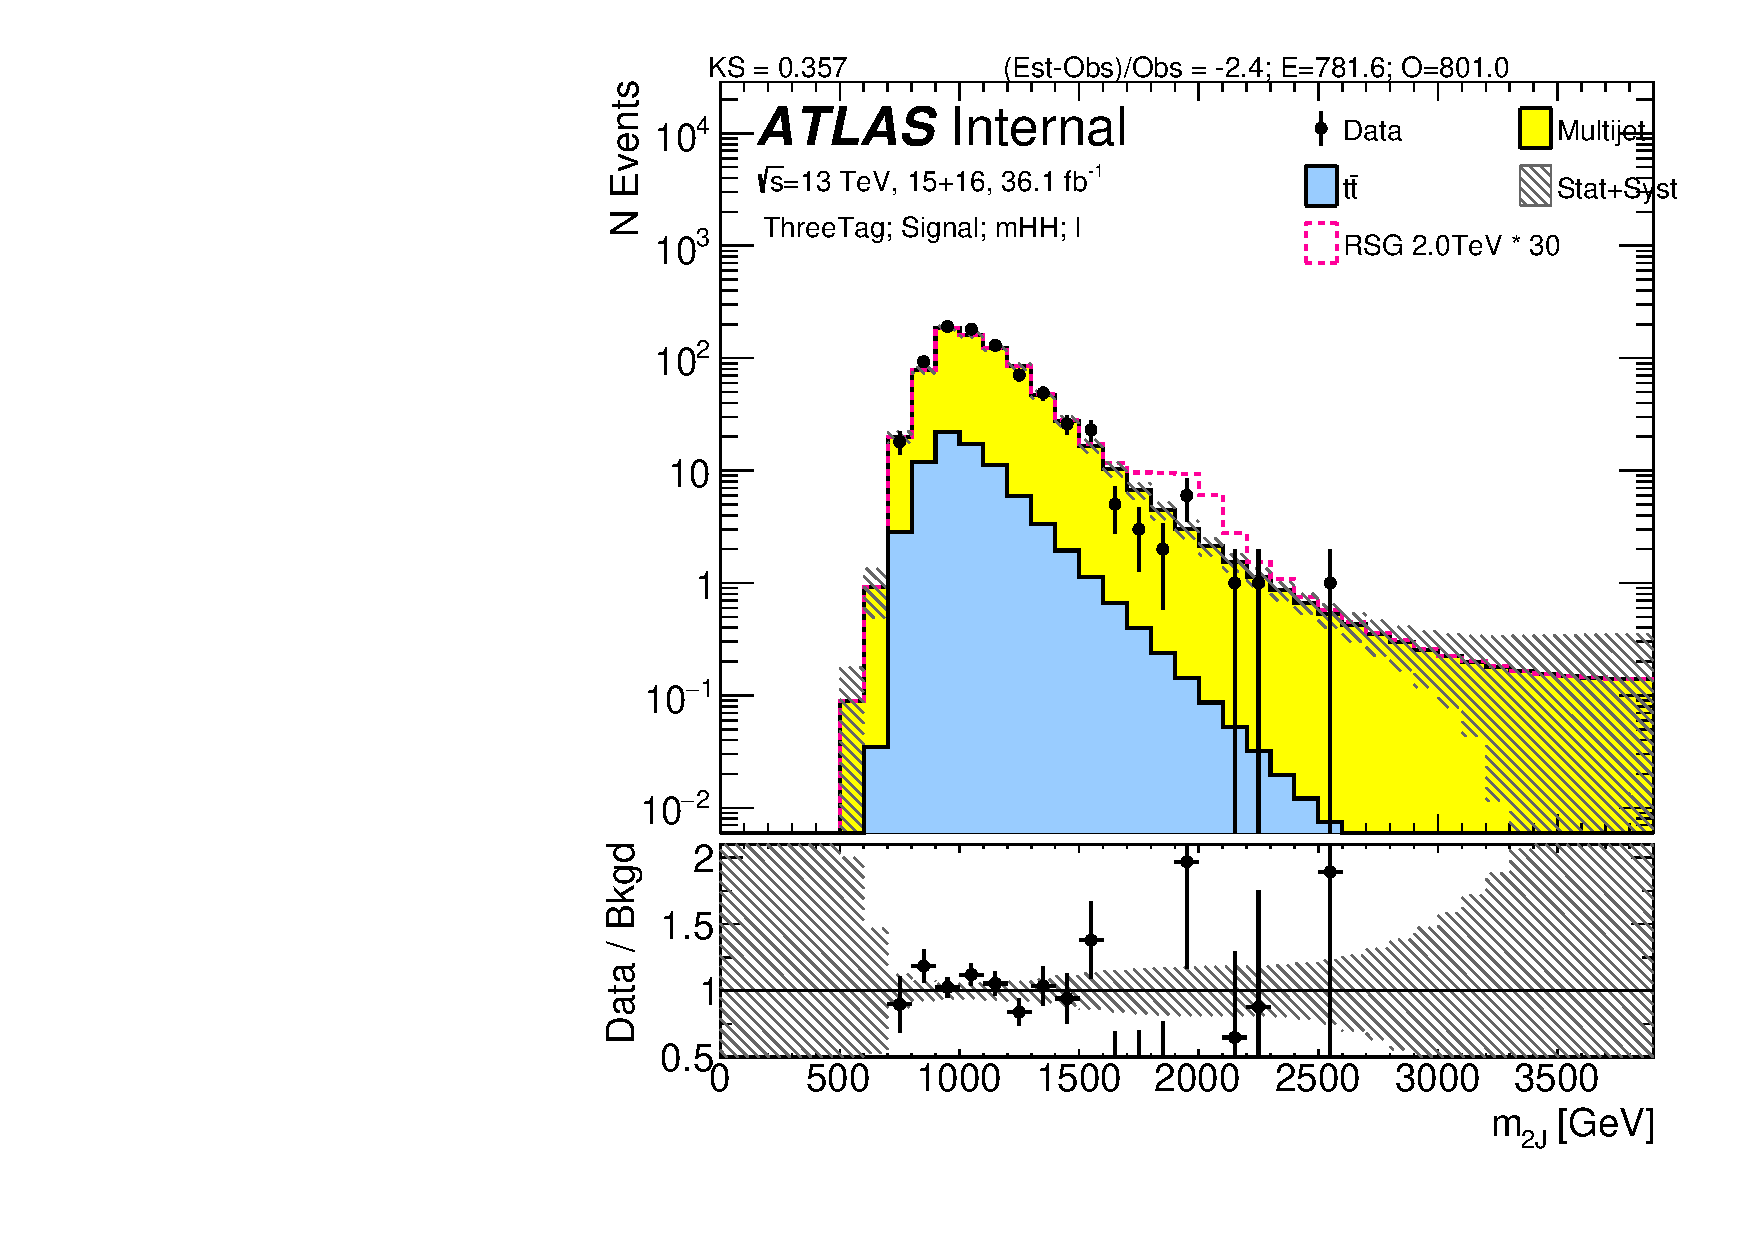
\includegraphics[width=\textwidth,angle=-90]{figures/boosted/Signal_Syst/Moriond_bkg_9_ThreeTag_Signal_mHH_l_1.pdf}
        \caption{Log-$y$}
        \label{fig:boosted-3b-signal-log}
    \end{subfigure}
  \caption{Unscaled \mtwoJ~ distribution in the $3b$ signal region after unblinding.}
  \label{fig:boosted-3b-signal-l}
\end{center}
\end{figure*}

\begin{figure*}[htb!]
\begin{center}
    \captionsetup{justification=centering}
    \begin{subfigure}[b]{0.45\textwidth}
        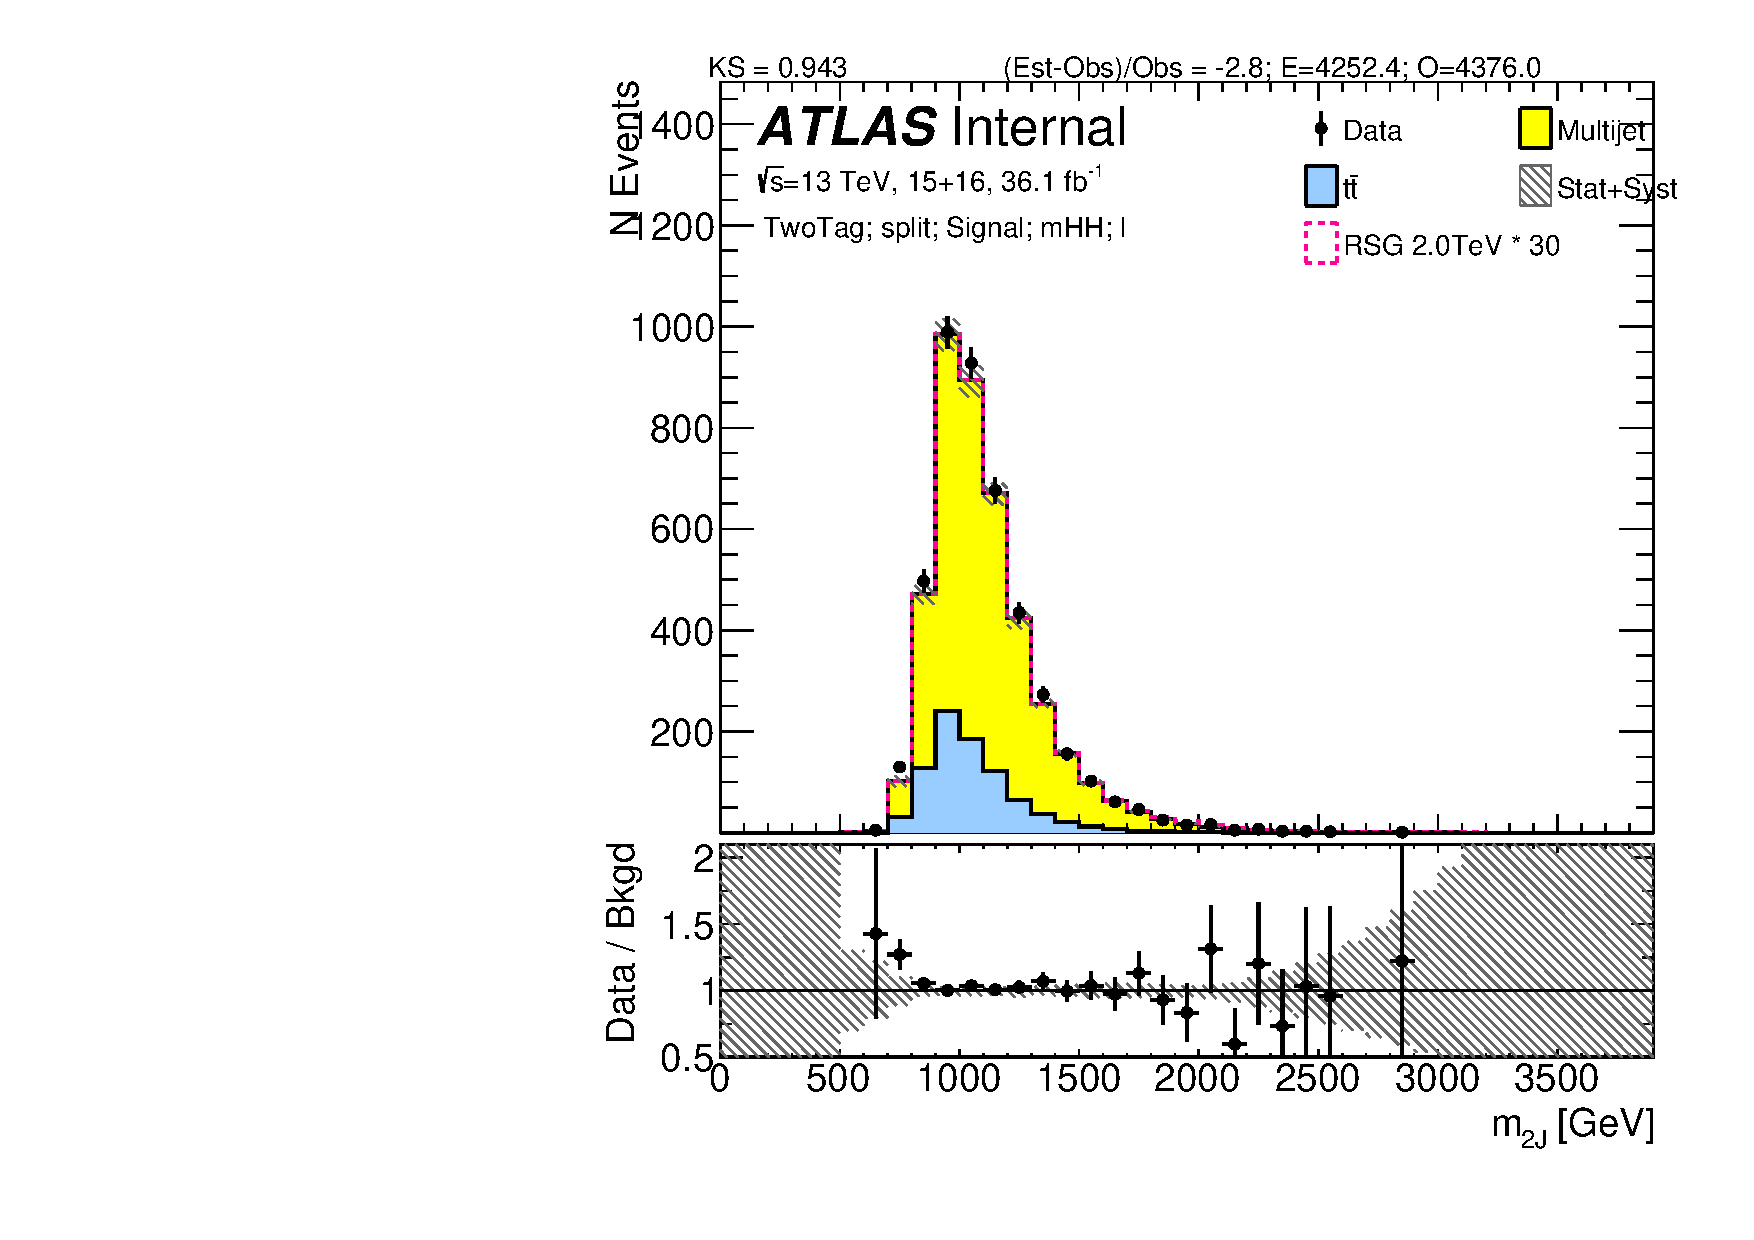
\includegraphics[width=\textwidth,angle=-90]{figures/boosted/Signal_Syst/Moriond_bkg_9_TwoTag_split_Signal_mHH_l.pdf}
        \caption{Linear-$y$}
        \label{fig:boosted-2b-signal-lin}
    \end{subfigure}
    \quad
    \begin{subfigure}[b]{0.45\textwidth}
        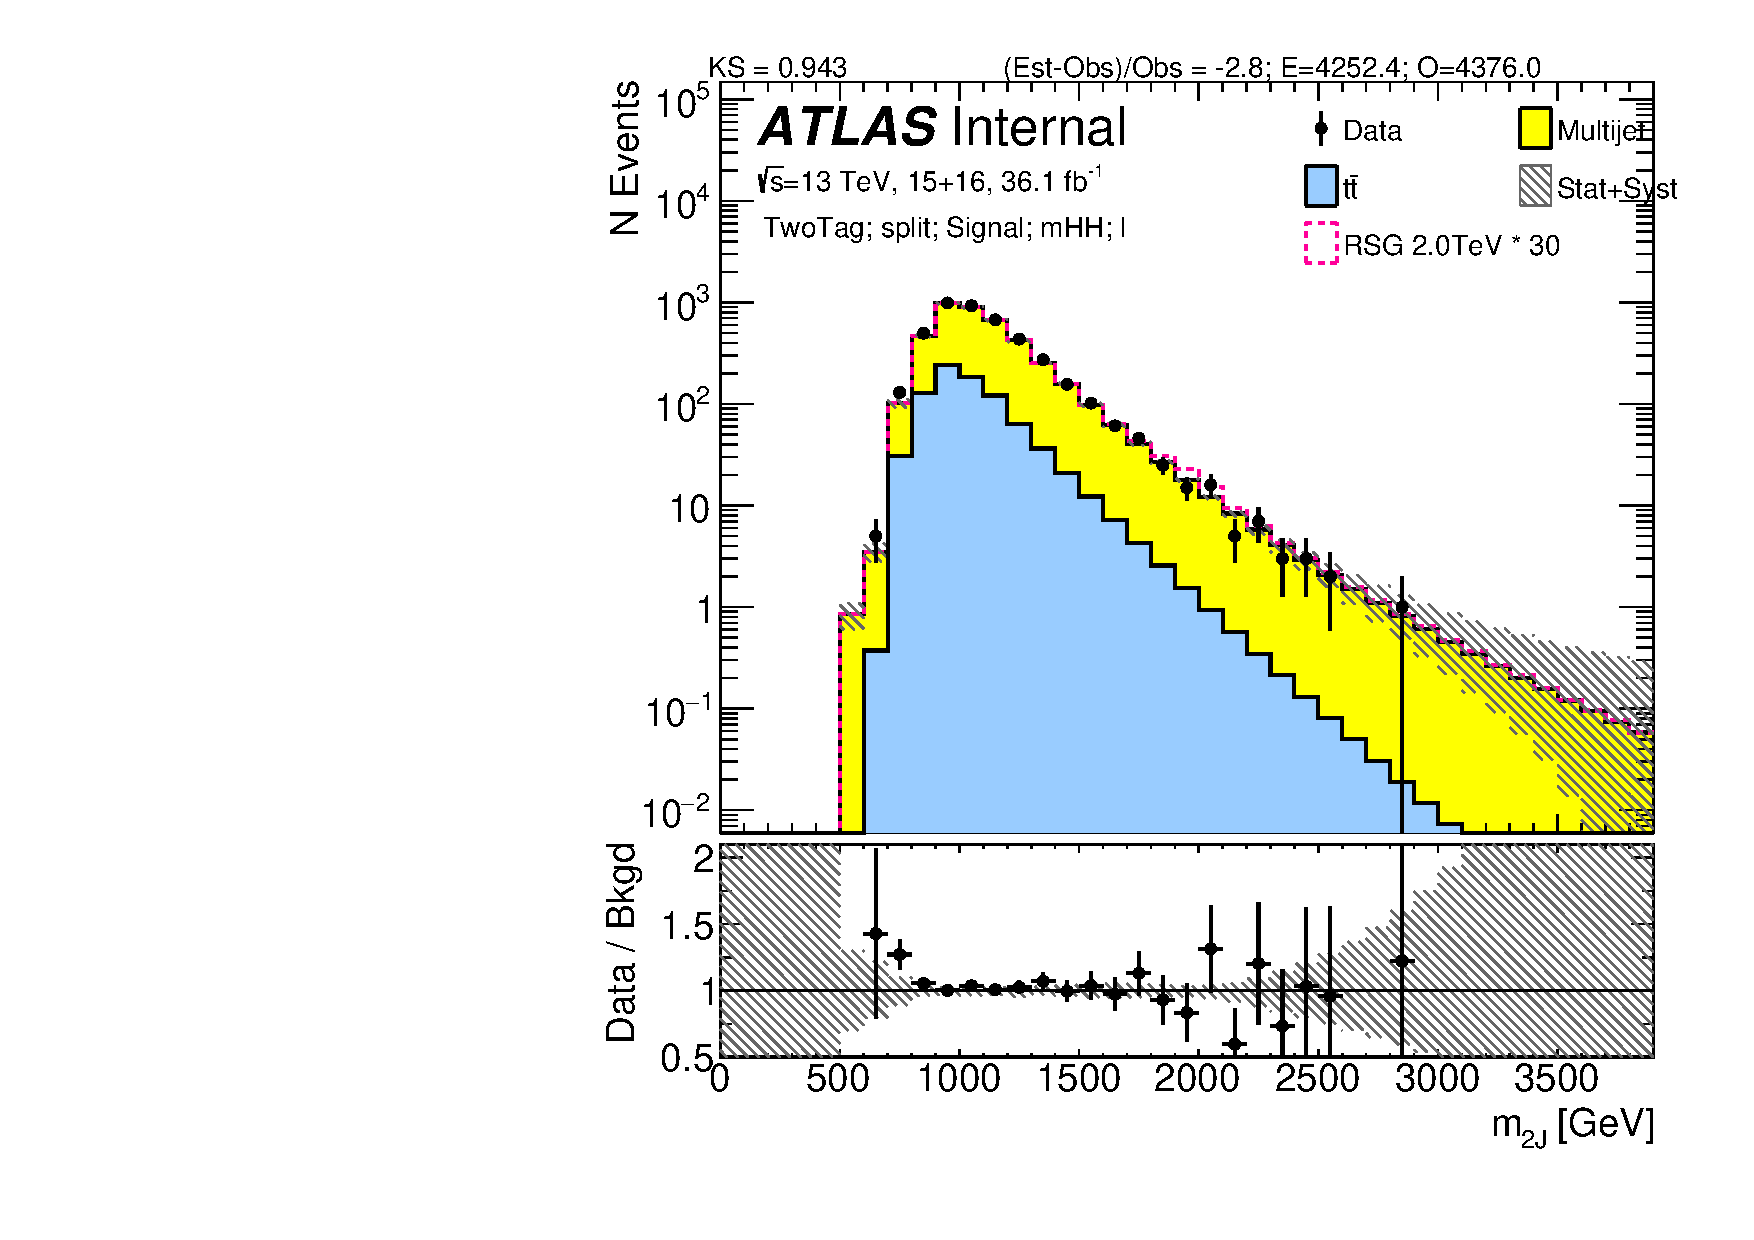
\includegraphics[width=\textwidth,angle=-90]{figures/boosted/Signal_Syst/Moriond_bkg_9_TwoTag_split_Signal_mHH_l_1.pdf}
        \caption{Log-$y$}
        \label{fig:boosted-2b-signal-log}
    \end{subfigure}
  \caption{Unscaled \mtwoJ~ distribution in the $2bs$ signal region after unblinding.}
  \label{fig:boosted-2b-signal-l}
\end{center}
\end{figure*}


\begin{figure*}[htb!]
\begin{center}
    \captionsetup{justification=centering}
    \begin{subfigure}[b]{0.45\textwidth}
        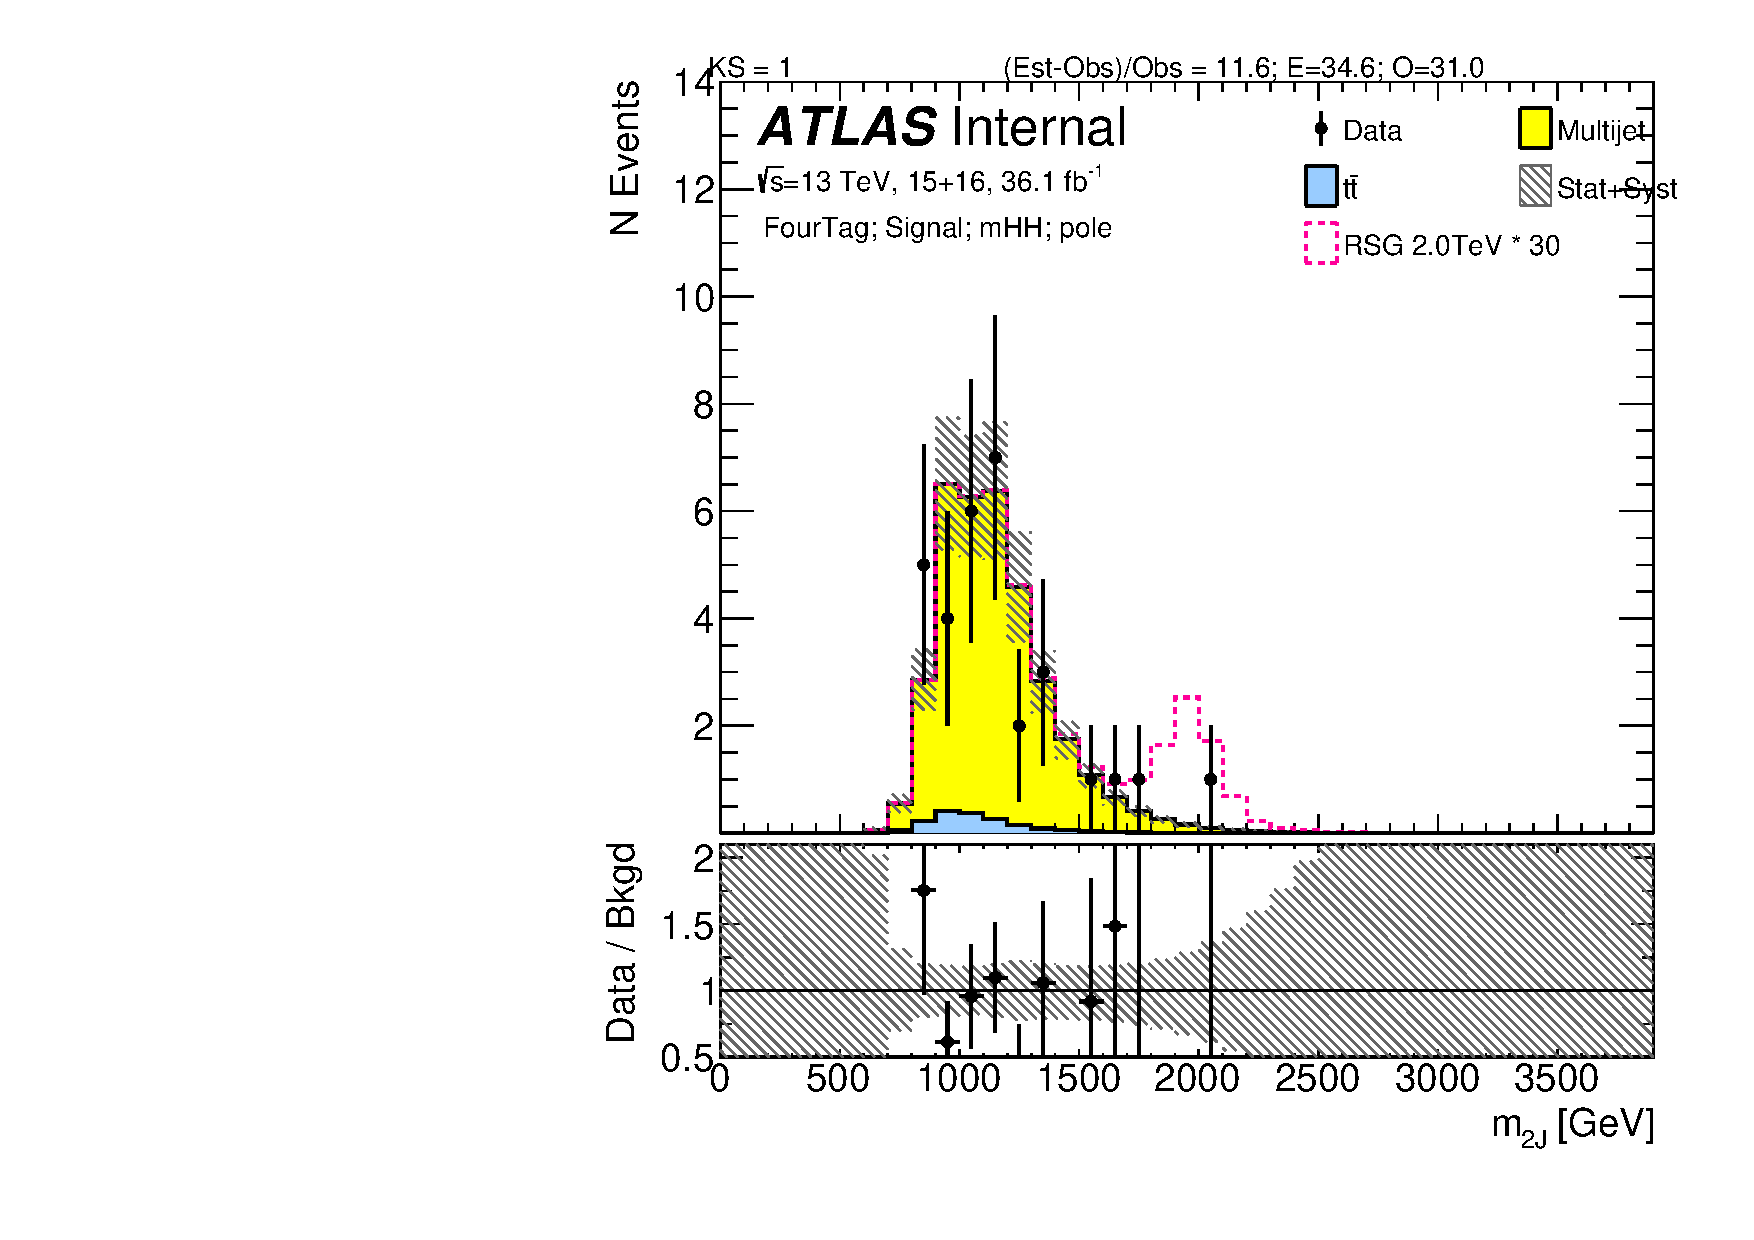
\includegraphics[width=\textwidth,angle=-90]{figures/boosted/Signal_Syst/Moriond_bkg_9_FourTag_Signal_mHH_pole.pdf}
        \caption{Linear-$y$}
        \label{fig:boosted-4b-signal-pole-lin}
    \end{subfigure}
    \quad
    \begin{subfigure}[b]{0.45\textwidth}
        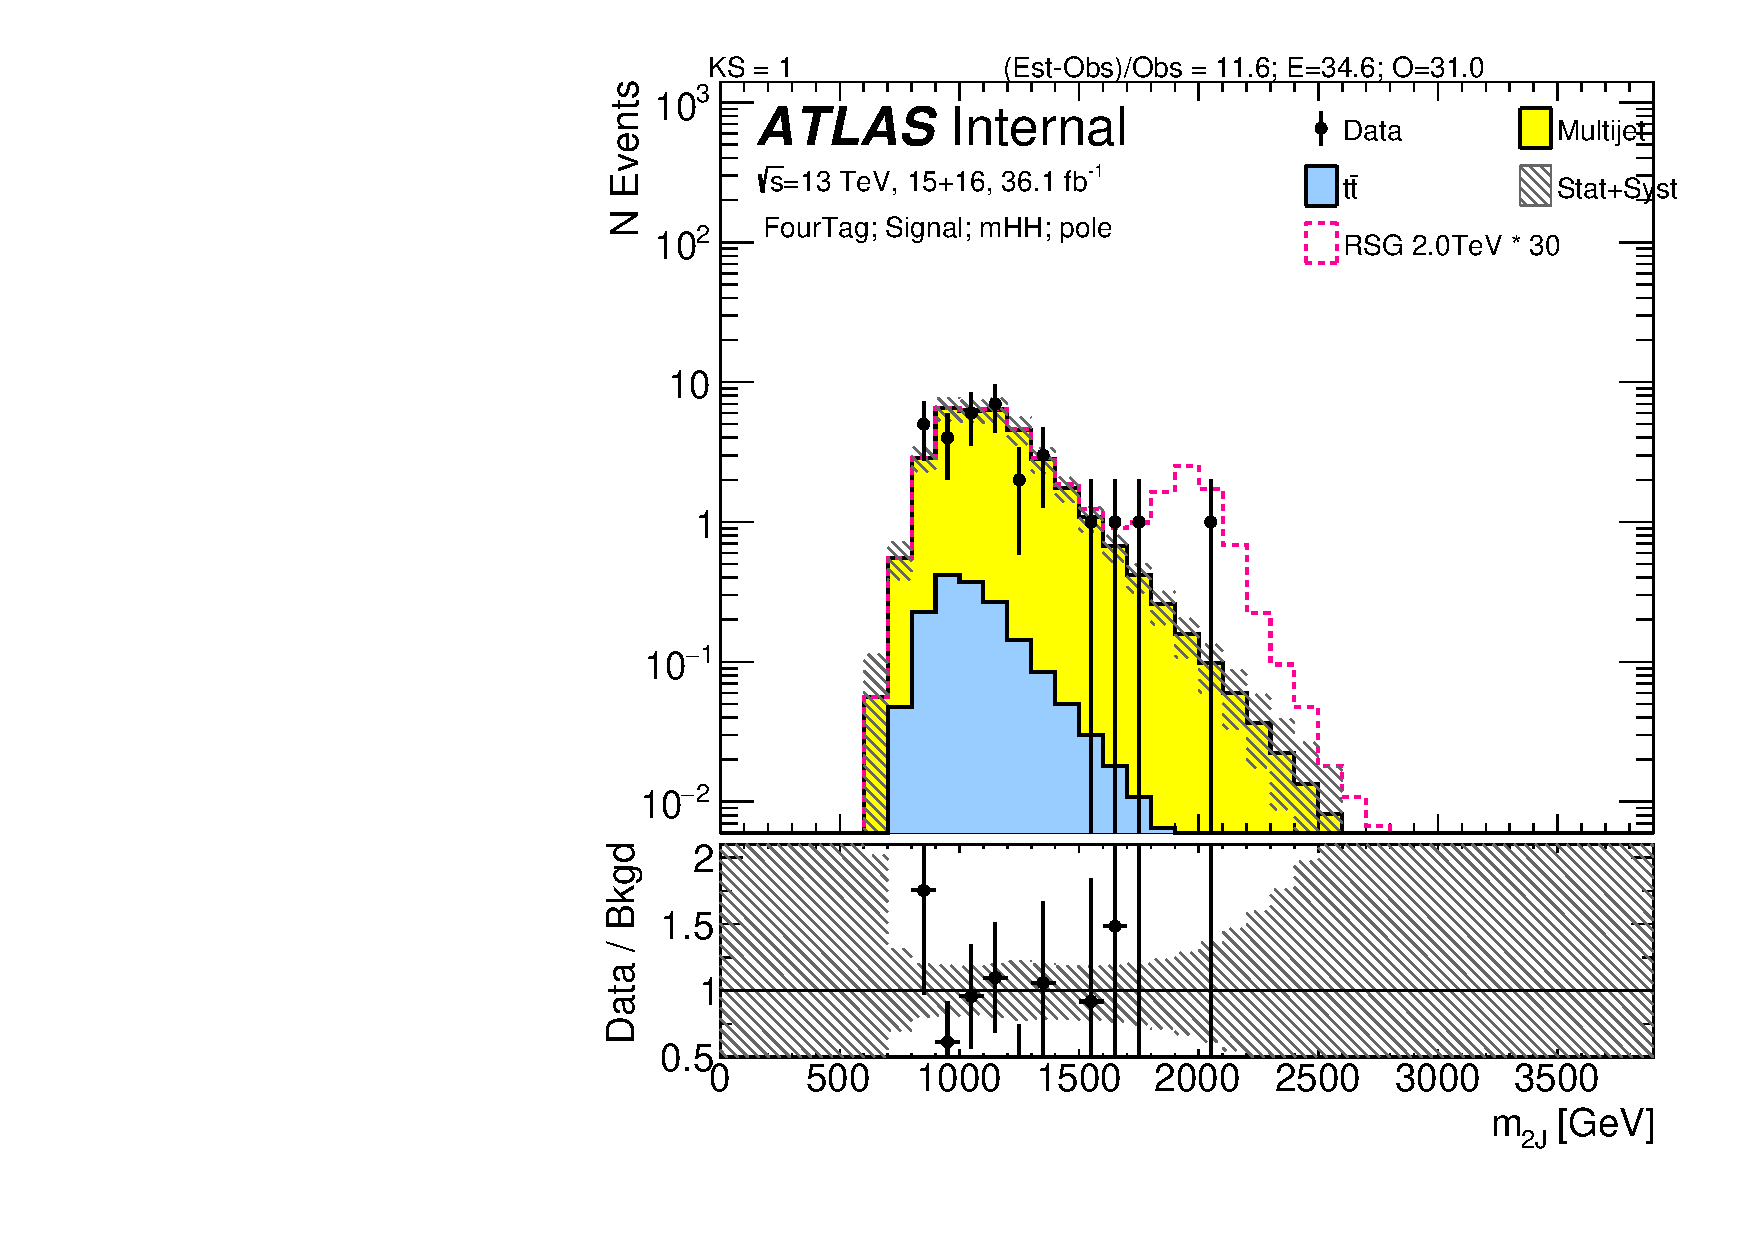
\includegraphics[width=\textwidth,angle=-90]{figures/boosted/Signal_Syst/Moriond_bkg_9_FourTag_Signal_mHH_pole_1.pdf}
        \caption{Log-$y$}
        \label{fig:boosted-4b-signal-pole-log}
    \end{subfigure}
  \caption{Scaled \mtwoJ~ distribution in the $4b$ signal region after unblinding.}
  \label{fig:boosted-4b-signal-pole}
\end{center}
\end{figure*}


\begin{figure*}[htb!]
\begin{center}
    \captionsetup{justification=centering}
    \begin{subfigure}[b]{0.45\textwidth}
        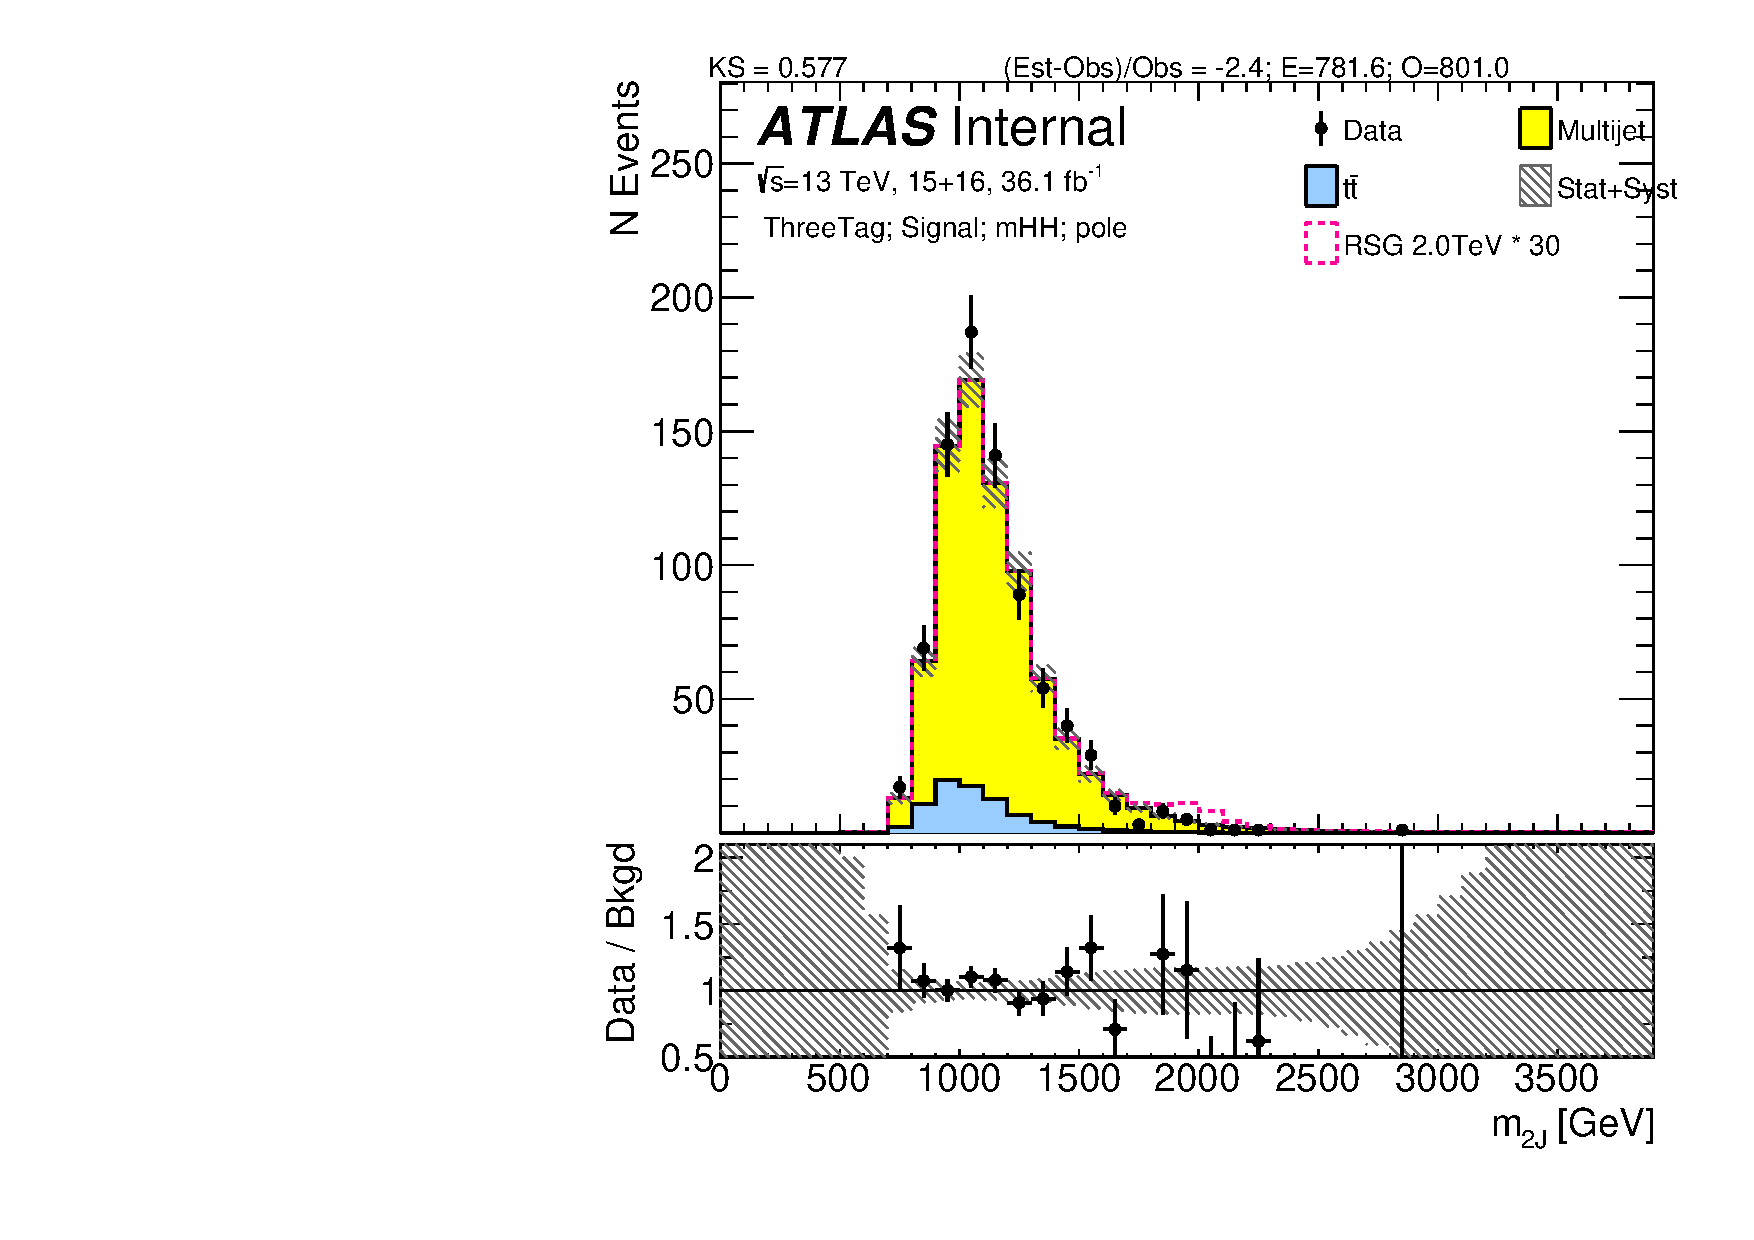
\includegraphics[width=\textwidth,angle=-90]{figures/boosted/Signal_Syst/Moriond_bkg_9_ThreeTag_Signal_mHH_pole.pdf}
        \caption{Linear-$y$}
        \label{fig:boosted-3b-signal-pole-lin}
    \end{subfigure}
    \quad
    \begin{subfigure}[b]{0.45\textwidth}
        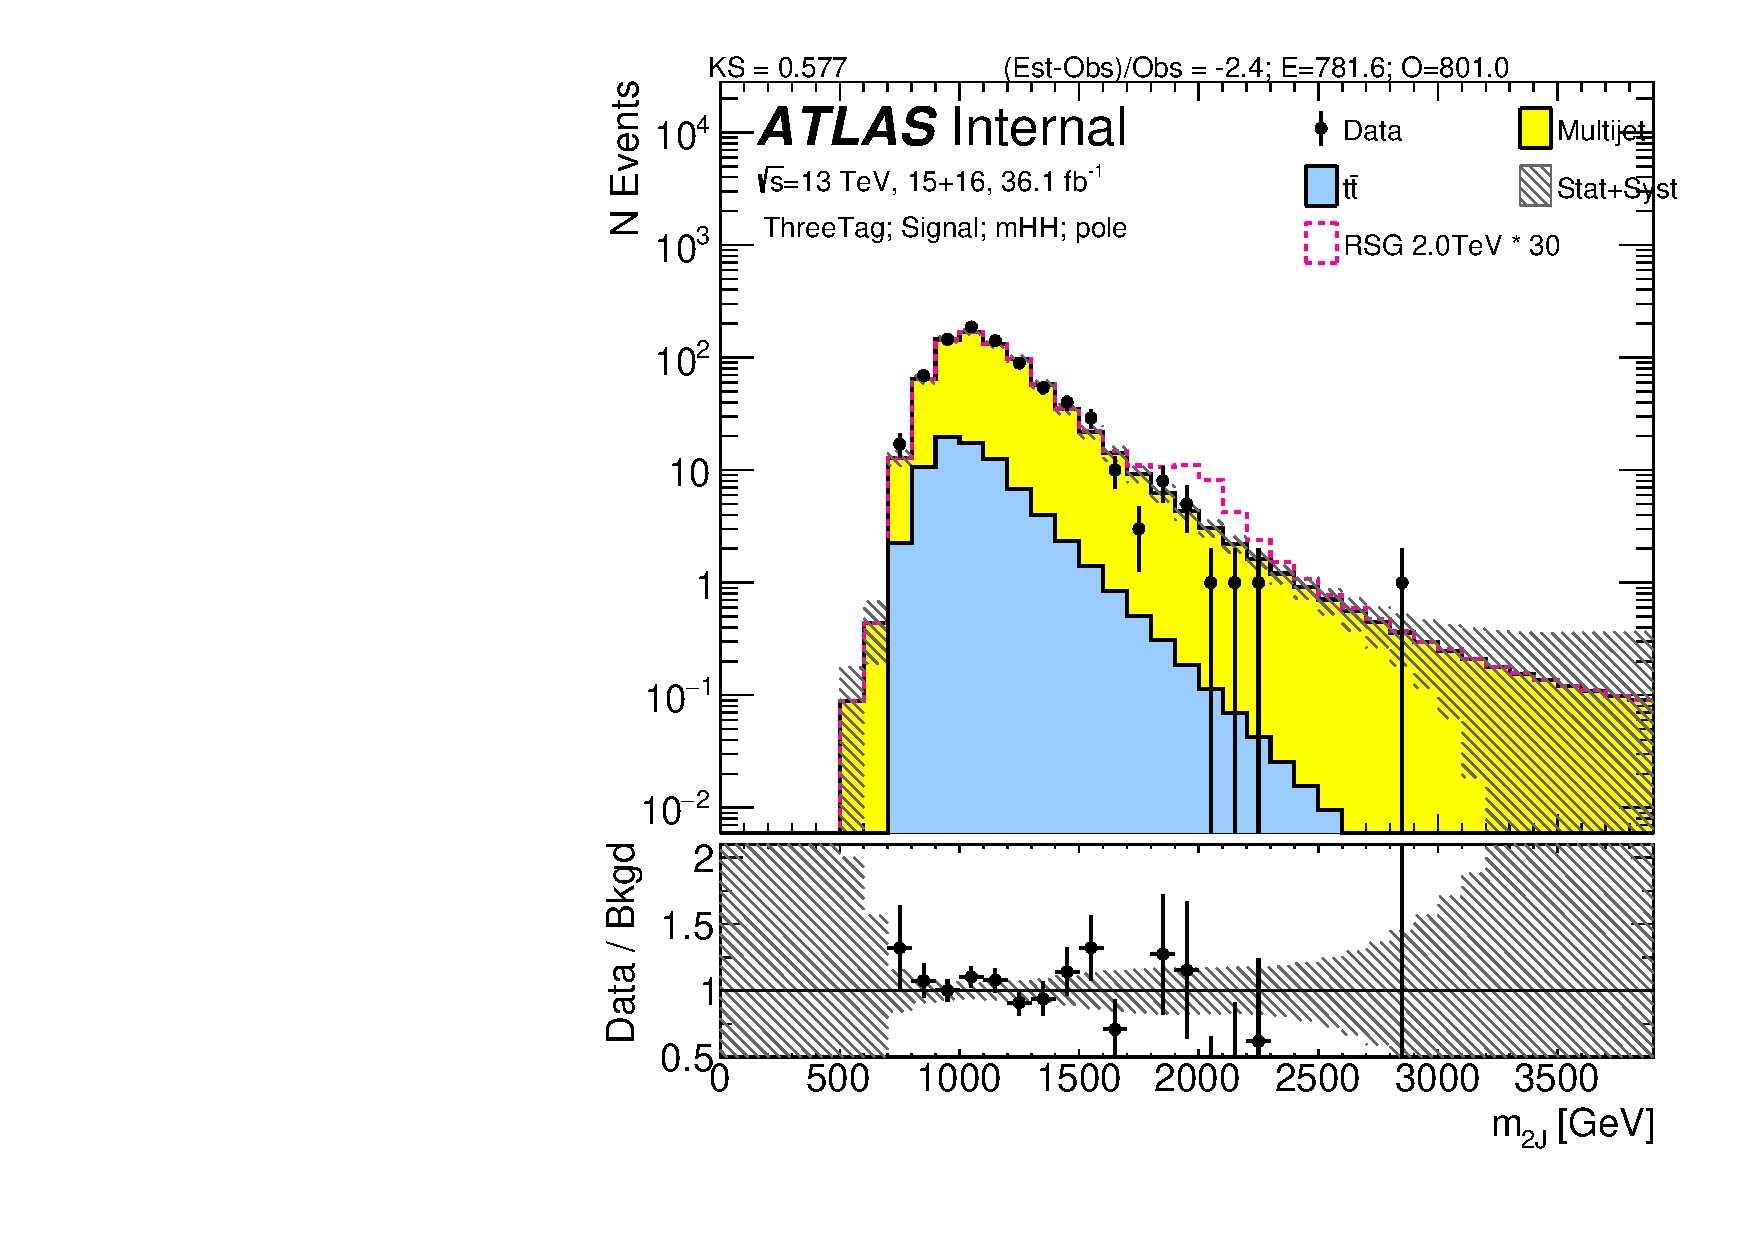
\includegraphics[width=\textwidth,angle=-90]{figures/boosted/Signal_Syst/Moriond_bkg_9_ThreeTag_Signal_mHH_pole_1.pdf}
        \caption{Log-$y$}
        \label{fig:boosted-3b-signal-pole-log}
    \end{subfigure}
  \caption{Scaled \mtwoJ~ distribution in the $3b$ signal region after unblinding.}
  \label{fig:boosted-3b-signal-pole}
\end{center}
\end{figure*}

\begin{figure*}[htb!]
\begin{center}
    \captionsetup{justification=centering}
    \begin{subfigure}[b]{0.45\textwidth}
        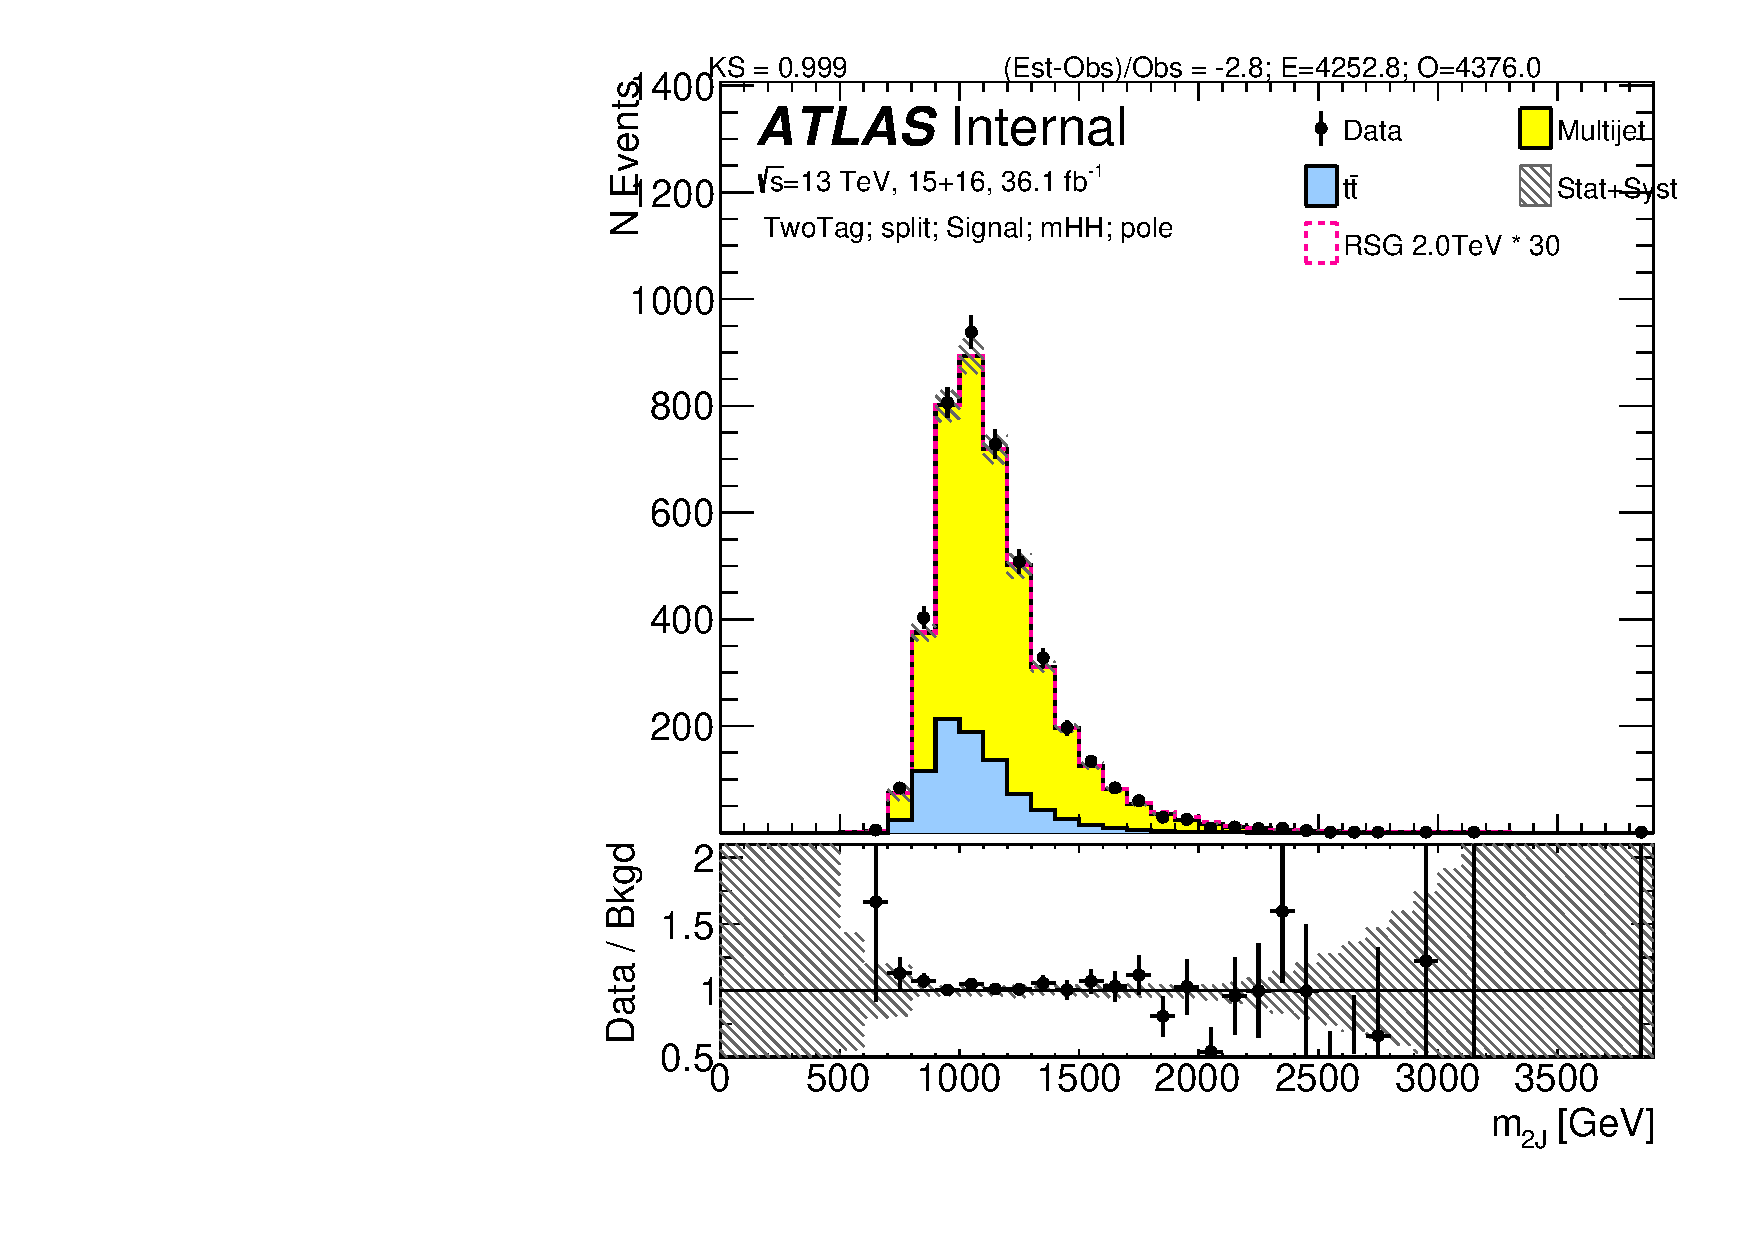
\includegraphics[width=\textwidth,angle=-90]{figures/boosted/Signal_Syst/Moriond_bkg_9_TwoTag_split_Signal_mHH_pole.pdf}
        \caption{Linear-$y$}
        \label{fig:boosted-2b-signal-pole-lin}
    \end{subfigure}
    \quad
    \begin{subfigure}[b]{0.45\textwidth}
        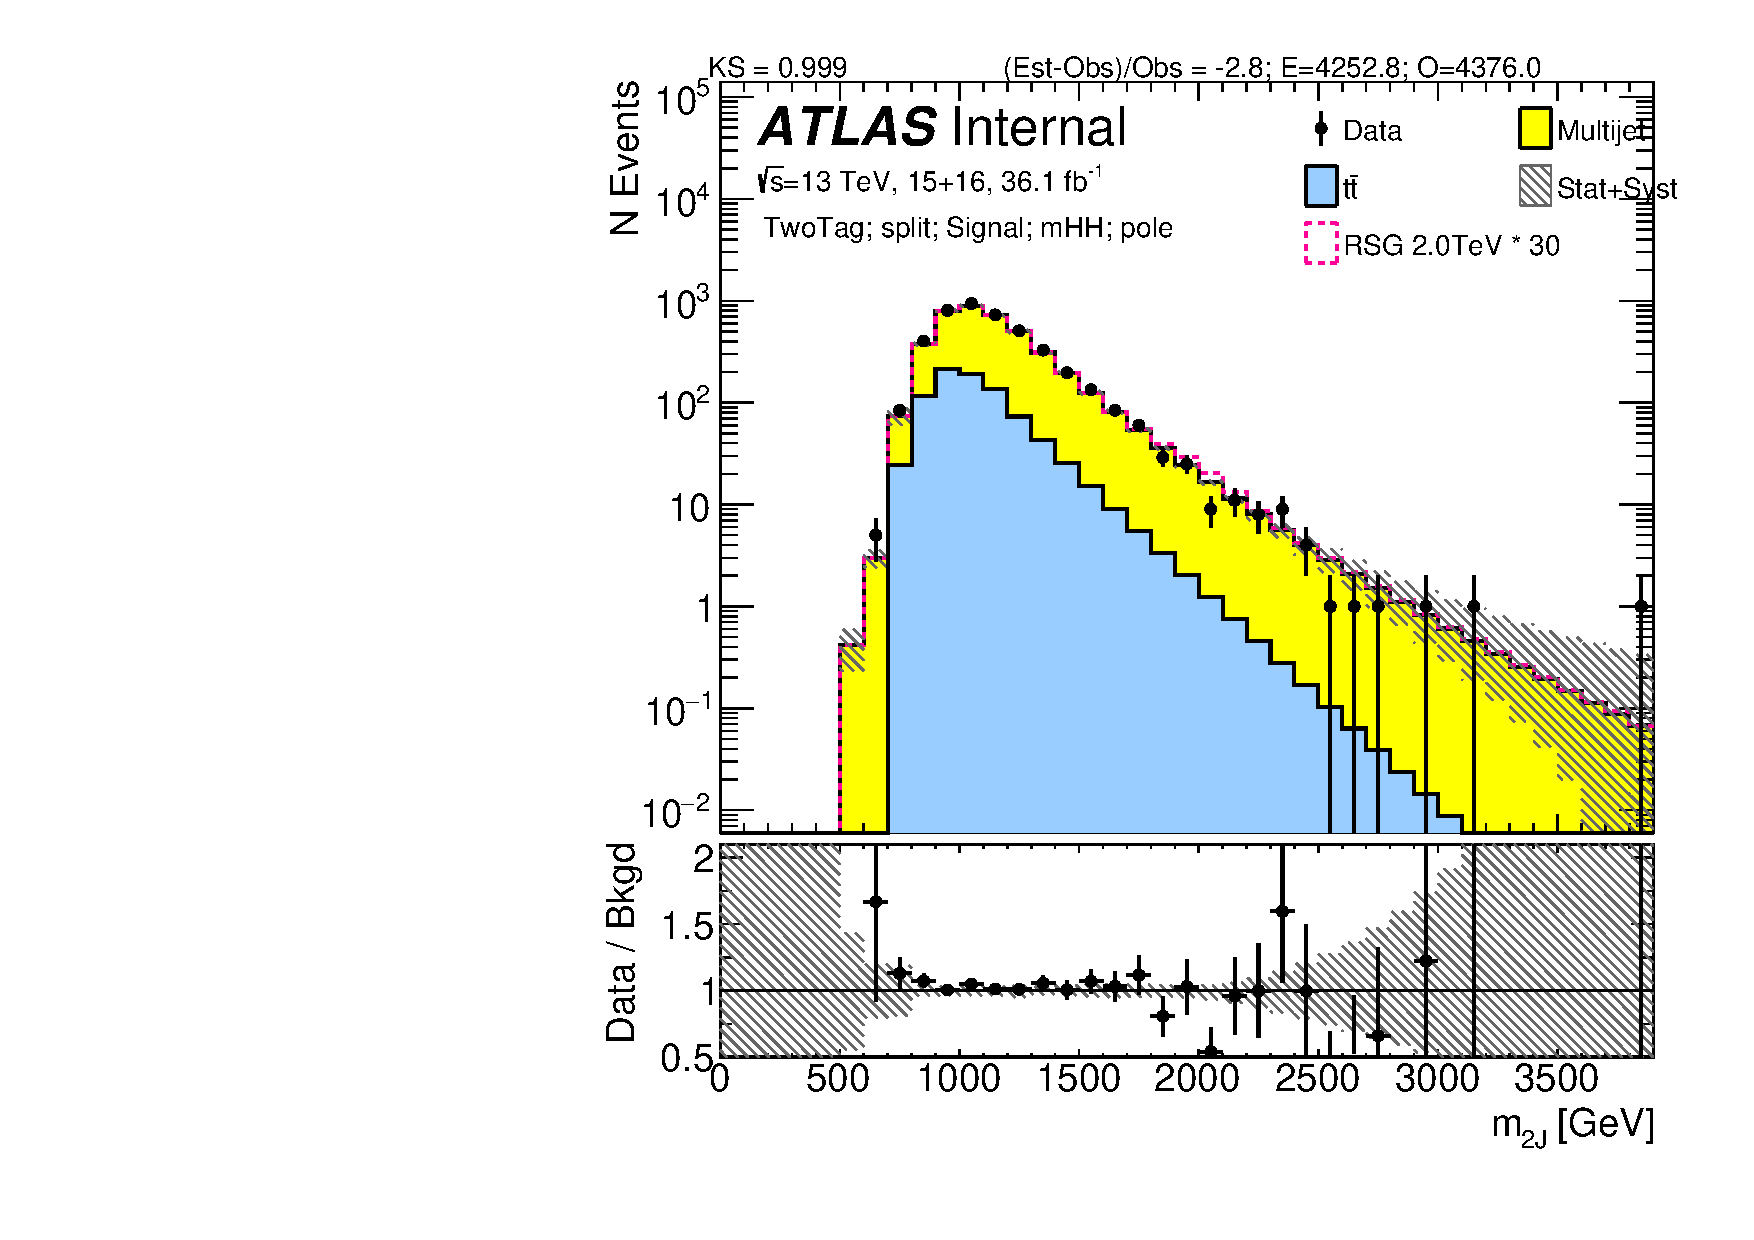
\includegraphics[width=\textwidth,angle=-90]{figures/boosted/Signal_Syst/Moriond_bkg_9_TwoTag_split_Signal_mHH_pole_1.pdf}
        \caption{Log-$y$}
        \label{fig:boosted-2b-signal-pole-log}
    \end{subfigure}
  \caption{Scaled \mtwoJ~ distribution in the $2bs$ signal region after unblinding.}
  \label{fig:boosted-2b-signal-pole}
\end{center}
\end{figure*}

\section{Resolved signal region}
\label{sec:res-resolvedsr}
\paragraph{}
The number of events observed in the data, the predicted number of background events in the signal region, and the predicted yield for three potential signals are presented in Table~\ref{tab:resolvedResults} for both the 2015 and 2016 datasets. 
The numbers of observed and predicted events in the control region are also shown.
A discrepancy between data and the total prediction is seen in the 2016 dataset; about half of this excess can be attributed to one bin at $\mfourj=280$~\GeV.
This could be a trigger turn-on effect.

\begin{table}[!ht]
\begin{center}
\caption{The number of predicted background events in the signal region for the resolved analysis compared to the data, for the 2015 and 2016 datasets. The yields for three potential signals, an $800$~\GeV\ \Grav~ resonance with $c = 1$, a scalar with a mass of $280$~\GeV, and SM non-resonant Higgs boson pair production, are also shown. The scalar sample is normalized to a cross section times branching ratio of $2.7$ pb. The quoted uncertainties include both the statistical and systematic uncertainties, and the total uncertainty considers correlations. The numbers of observed and predicted events are also given in the control region.}

\begin{tabular}{c|c|c|c|c} 
Sample & 2015 SR & 2016 SR & 2015 CR & 2016 CR\\
Multijet                & 866     $\pm$  70      &  6750 $\pm$ 170  & 880 $\pm$ 71 & 7110 $\pm$ 180 \\
\ttbar, hadronic        &  52     $\pm$  35      & 259   $\pm$ 57   & 56  $\pm$ 37 & 276  $\pm$ 61 \\
\ttbar, leptonic    &  13.9   $\pm$  6.5     &  123  $\pm$  30  & 20  $\pm$ 9  & 168 $\pm$ 40 \\
Total         & 930 $\pm$ 70      & 7130 $\pm$ 130  & 956 $\pm$ 50 &  7550 $\pm$ 130 \\
Data         & 928    & 7430 & 969 &7656  \\
\Grav$\left(800~\GeV\right)$ & 12.5   & 1.9     &  89  & 14 \\
Scalar (280~\GeV)            & 24     & 7.5     & 180  & 57 \\
SM di-Higgs                       & 0.607  & 0.091   & 4.43 & 0.66 \\
\end{tabular}
\label{tab:resolvedResults}
\end{center}
\end{table}

\paragraph{}
Figure~\ref{fig:resolvedHHUnblinded} shows comparisons of the predicted \mfourj~ background distributions to those observed in the 2015 and 2016 datasets. 
A few signal models are also displayed. 
The scalar sample shown is normalized to a cross section times \hbb~ branching ratio of $2.7$~pb, which is the best-fit value. 
The predicted background and observed distributions are mostly in agreement, with an excess above the predicted background in one bin around $280$~\GeV.


\begin{figure*}[htb!]
\begin{center}
    \captionsetup{justification=centering}
    \hspace{-2cm}
    \begin{subfigure}[b]{0.39\textwidth}
        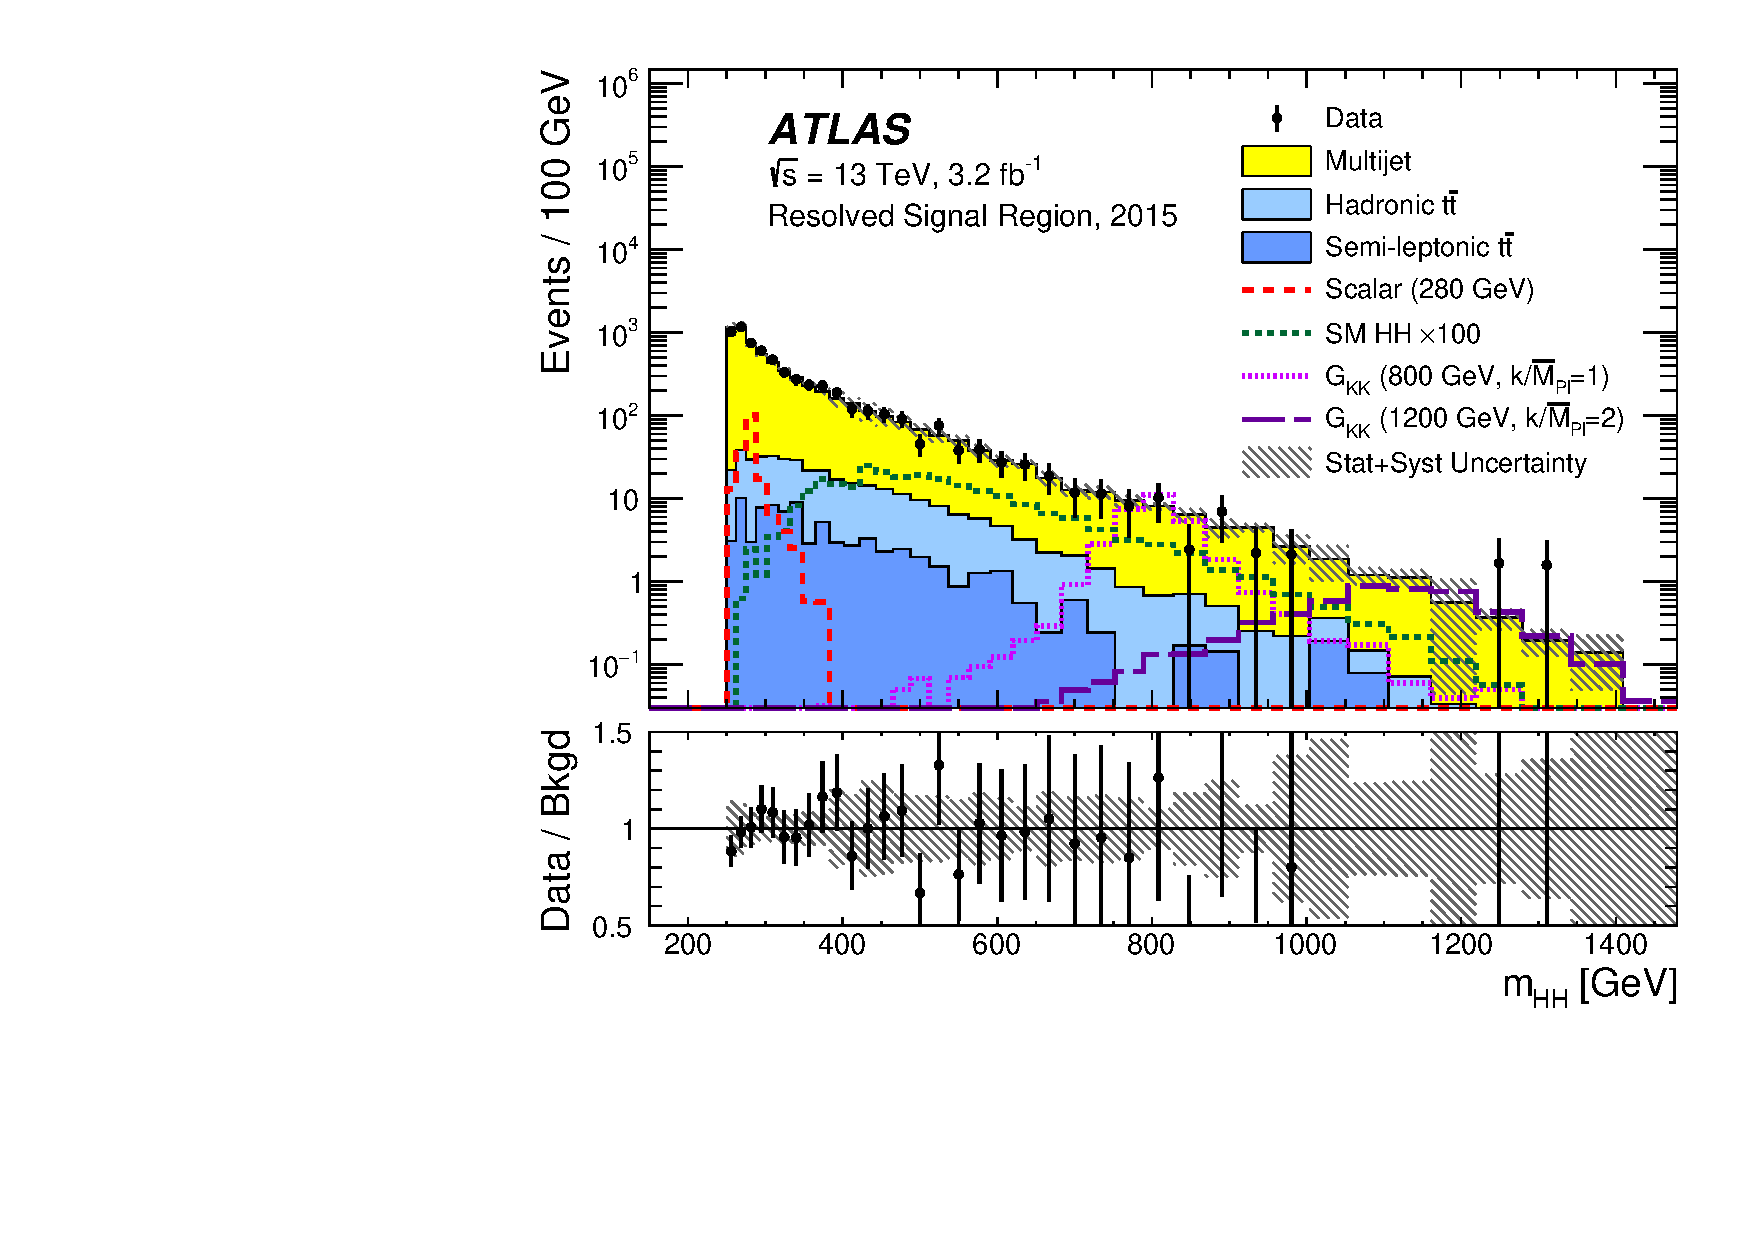
\includegraphics[width=\textwidth,angle=-90]{figures/resolved/results/data_2015_hh_v_logy.pdf}
        \caption{2015}
        \label{fig:resolvedHHUnblinded-2015}
    \end{subfigure}
    \quad \quad \quad
    \begin{subfigure}[b]{0.39\textwidth}
        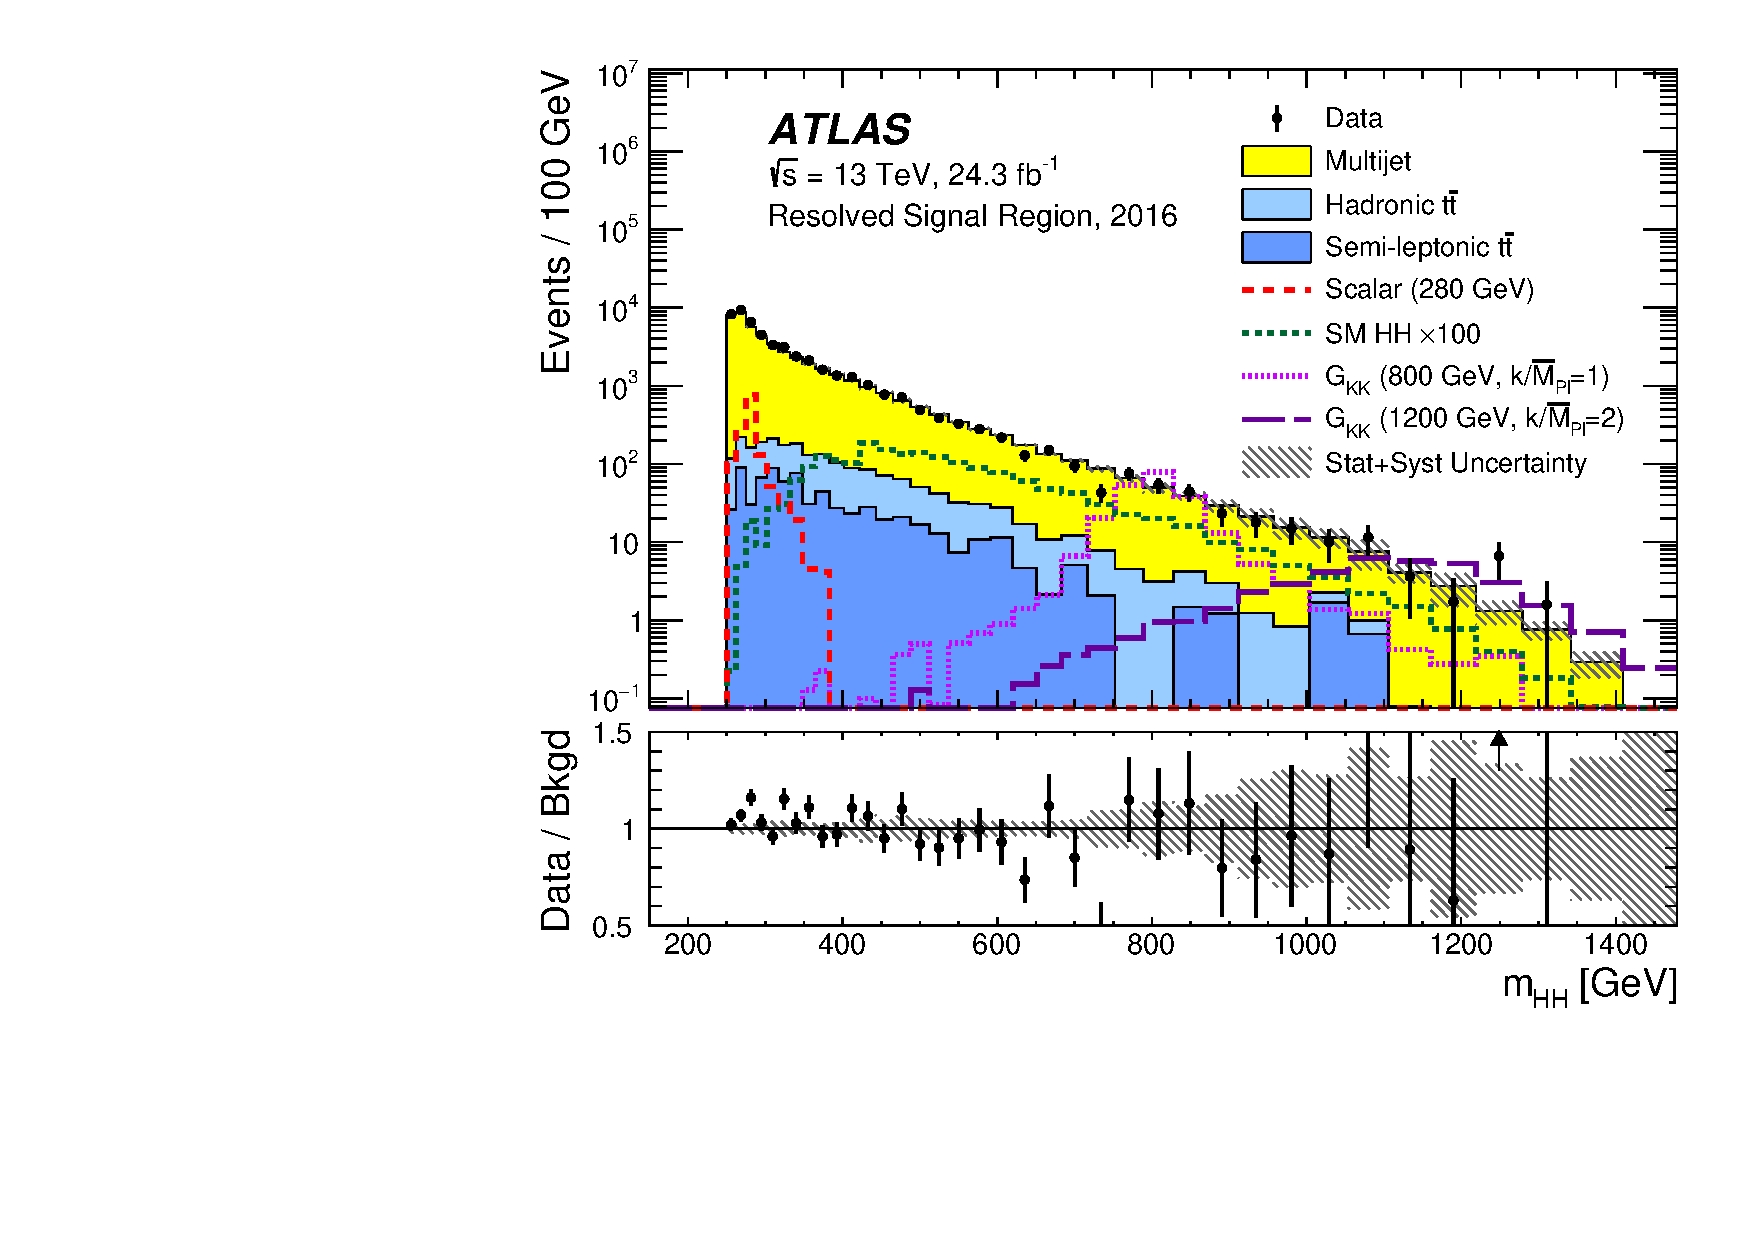
\includegraphics[width=\textwidth,angle=-90]{figures/resolved/results/data_2016_hh_v_logy.pdf}
        \caption{2016}
        \label{fig:resolvedHHUnblinded-2016}
    \end{subfigure}
  \caption{Distributions of \mfourj in the signal region of the resolved analysis for (a) 2015 data and (b) 2016 data, compared to the predicted backgrounds. The hatched bands shown in the bottom panels represent the combined statistical and systematic uncertainties in the total background estimates. The expected signal distributions of \Grav~ resonances with masses of $800$ and $1200$~\GeV, the $280$~\GeV~ scalar sample and SM non-resonant di-Higgs production $(\times 100)$ are also shown. The scalar sample is normalized to a cross section times branching ratio of $2.7$~pb.}
  \label{fig:resolvedHHUnblinded}
\end{center}
\end{figure*}


\section{Statistical analysis}
\label{sec:observedlimits}

%  \paragraph{}
% To evaluate an upper limit of resonant signal cross section, a frequentist method is used where a cross section is excluded on the basis of the statistic \cls~\cite{Read:2002hq}, which is defined as the ratio of \clsb to \clb.
% \clsb is defined as $P_{s+b}(q \le q_{obs})$, i.e. the probability of the signal+background model to produce data with a value of q less than that observed.
% q is a test statistic, which tests the compatibility with the signal+background hypothesis, where low values indicate a high level of compatibility. 
% \clb = $P_{b}(q \le q_{obs})$, i.e. the probability of the background model to produce data with the same or more compatibility with the signal+background  model as that observed. 
% Cross sections are excluded if they have a value of \cls $\le 0.05$.
\paragraph{}
Following the statistical procedures outlined in Ref.~\cite{Aad:2012tfa}, a test statistic based on the profile likelihood ratio~\cite{Cowan:2010js} is used to test hypothesized values of $\mu=\sigma/\sigma_{\mathrm{model}}$, the global signal strength factor, separately for each signal model. 
The exclusion limits are computed using asymptotic formula~\cite{Cowan:2010js} and are based on the \cls method~\cite{Read:2002hq}, where a value of $\mu$ is regarded as excluded at the $95\%$ confidence level (CL) when \cls~is less than $5\%$.

\paragraph{}
The test statistic used is a one sided profile likelihood ratio:
\begin{eqnarray}
  {q_{0}} = -2 ln \frac{L(0,\hat{\hat{\theta}}(0))}{L(\hat{\mu},\hat{\theta})}; \hat{\mu} > 0 \\
  {q_{0}} =  0 ; \hat{\mu} < 0 
\end{eqnarray}
Where $\mu$ is the value of the signal normalization considered, $\hat{\mu}$ is the maximum likelihood (ML) value of $\mu$. 
$\theta$ is the set of nuisance parameters (NP): $\hat{\theta}$ is the ML value of $\theta$ and 
$\hat{\hat{\theta}}$ is the ML value of $\theta$ when $\mu$ is fixed at a particular value. 
$L$ denotes the profile likelihood: $L(\hat{\mu},\hat{\theta})$ is the likelihood where $\mu$ is allowed to take any value, the unconstrained likelihood. 
$L(0,\hat{\hat{\theta}}(0))$ is the likelihood for the value of $\mu = 0$, the constrained likelihood.

\paragraph{}
This tests the compatibility of the data with the background-only hypothesis, $\mu = 0$. 
The local p-value of a set of data, $p_0$, is defined as the probability for the 
background-only hypothesis to have a value of $q_0$ that is as high or higher than the 
value of $q_{0}$ in that data.
In order to obtain $p_0$, pseudo-experiments are generated with the background only 
model and the distribution of the test statistic, $q_{0}$, is built up from the 
values of the pseudo-experiments.

% If a local $p_{0}$ value is obtained that corresponds to a significance of greater than $3\sigma$ then a correction for the look elsewhere effect will  be computed in order to obtain the global p-value. 
% This correction is obtained using the distribution of the test statistic, $q_{0}$, in background only pseudo-experiments. 
% The average number of upwards crossings, $<N_{1\sigma}>$, across the mass range tested of $q_{0}$ at the value of $q_{0}$ corresponding to $1\sigma$ significance, $q_{0}^{1\sigma}$, 
% is estimated using the average number from the background only pseudo-experiments and is used to obtain the correction to the local p-value using the equation:
% \begin{equation}
%   p_{0}^{global} = p_{0}^{local} + <N_{1\sigma}>e^{-(q_{0}^{max} - q_{0}^{1\sigma})/2}
% \end{equation}
% \noindent
% Where $p_{0}^{local}$ is the lowest $p_{0}$ value across the mass range tested, 
% corresponding to a test statistic value of $q_{0}^{max}$. 

\paragraph{}
The background model is found to describe the data and no significant excess is observed. 
The smallest local $p_0=0.175$ (1$\sigma$) is found at $1100$ \GeV~ when fitting with the narrow scalar model. The local $p_0$ values for the three signal models as a function of the resonance mass are shown in Fig.~\ref{fig:localp0}.

\begin{figure*}[htb!]
\centering
\captionsetup{justification=centering}
    \hspace{-2.5cm}
    \begin{subfigure}[b]{0.35\textwidth}
        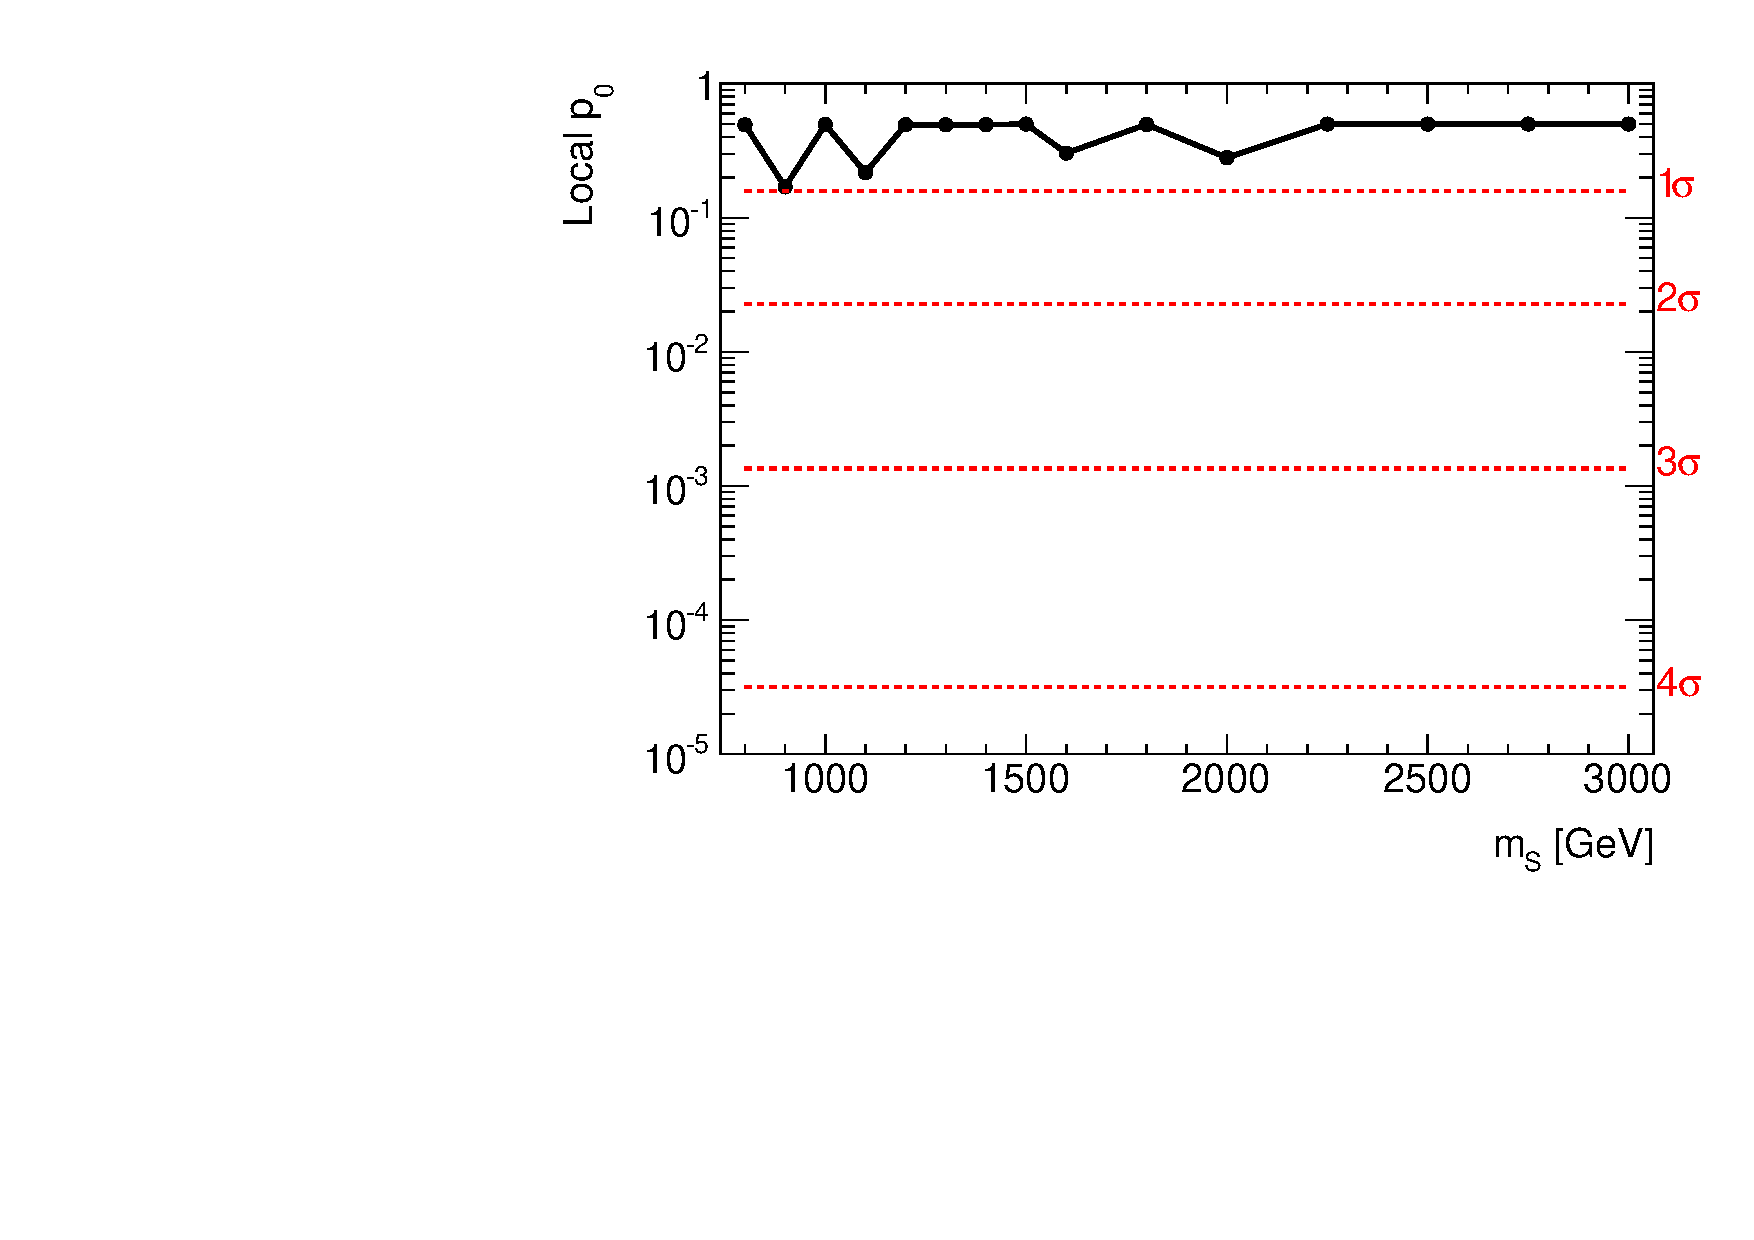
\includegraphics[width=\textwidth,angle=-90]{figures/boosted/results/p0_s_allmasses_boosted.pdf}
        \caption{scalar}
        \label{fig:localp0-s}
    \end{subfigure}
    \quad \quad \quad \quad \quad
    \begin{subfigure}[b]{0.35\textwidth}
        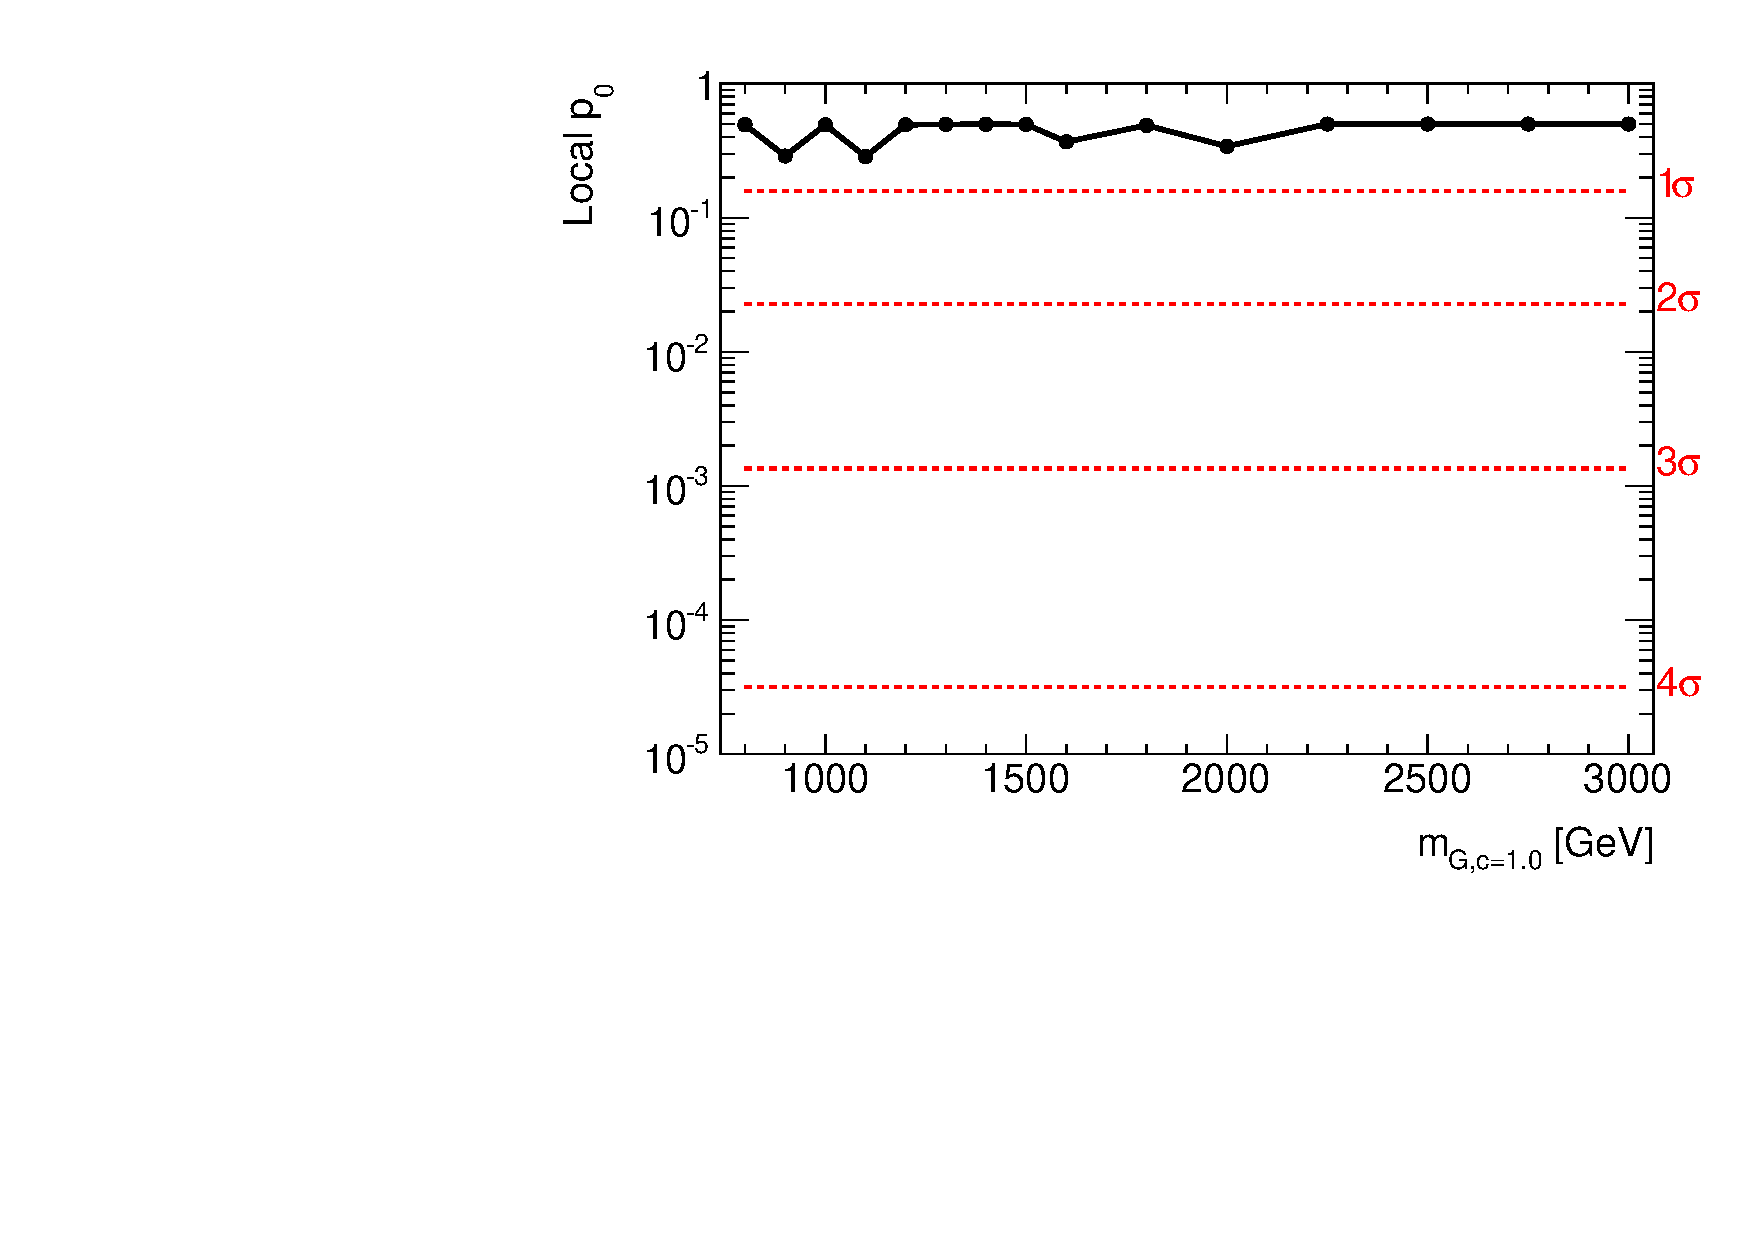
\includegraphics[width=\textwidth,angle=-90]{figures/boosted/results/p0_g10_allmasses_boosted.pdf}
        \caption{\Grav with $c=1$}
        \label{fig:localp0-g1}
    \end{subfigure}
    \\
    \hspace{-2.5cm}
    \begin{subfigure}[b]{0.35\textwidth}
        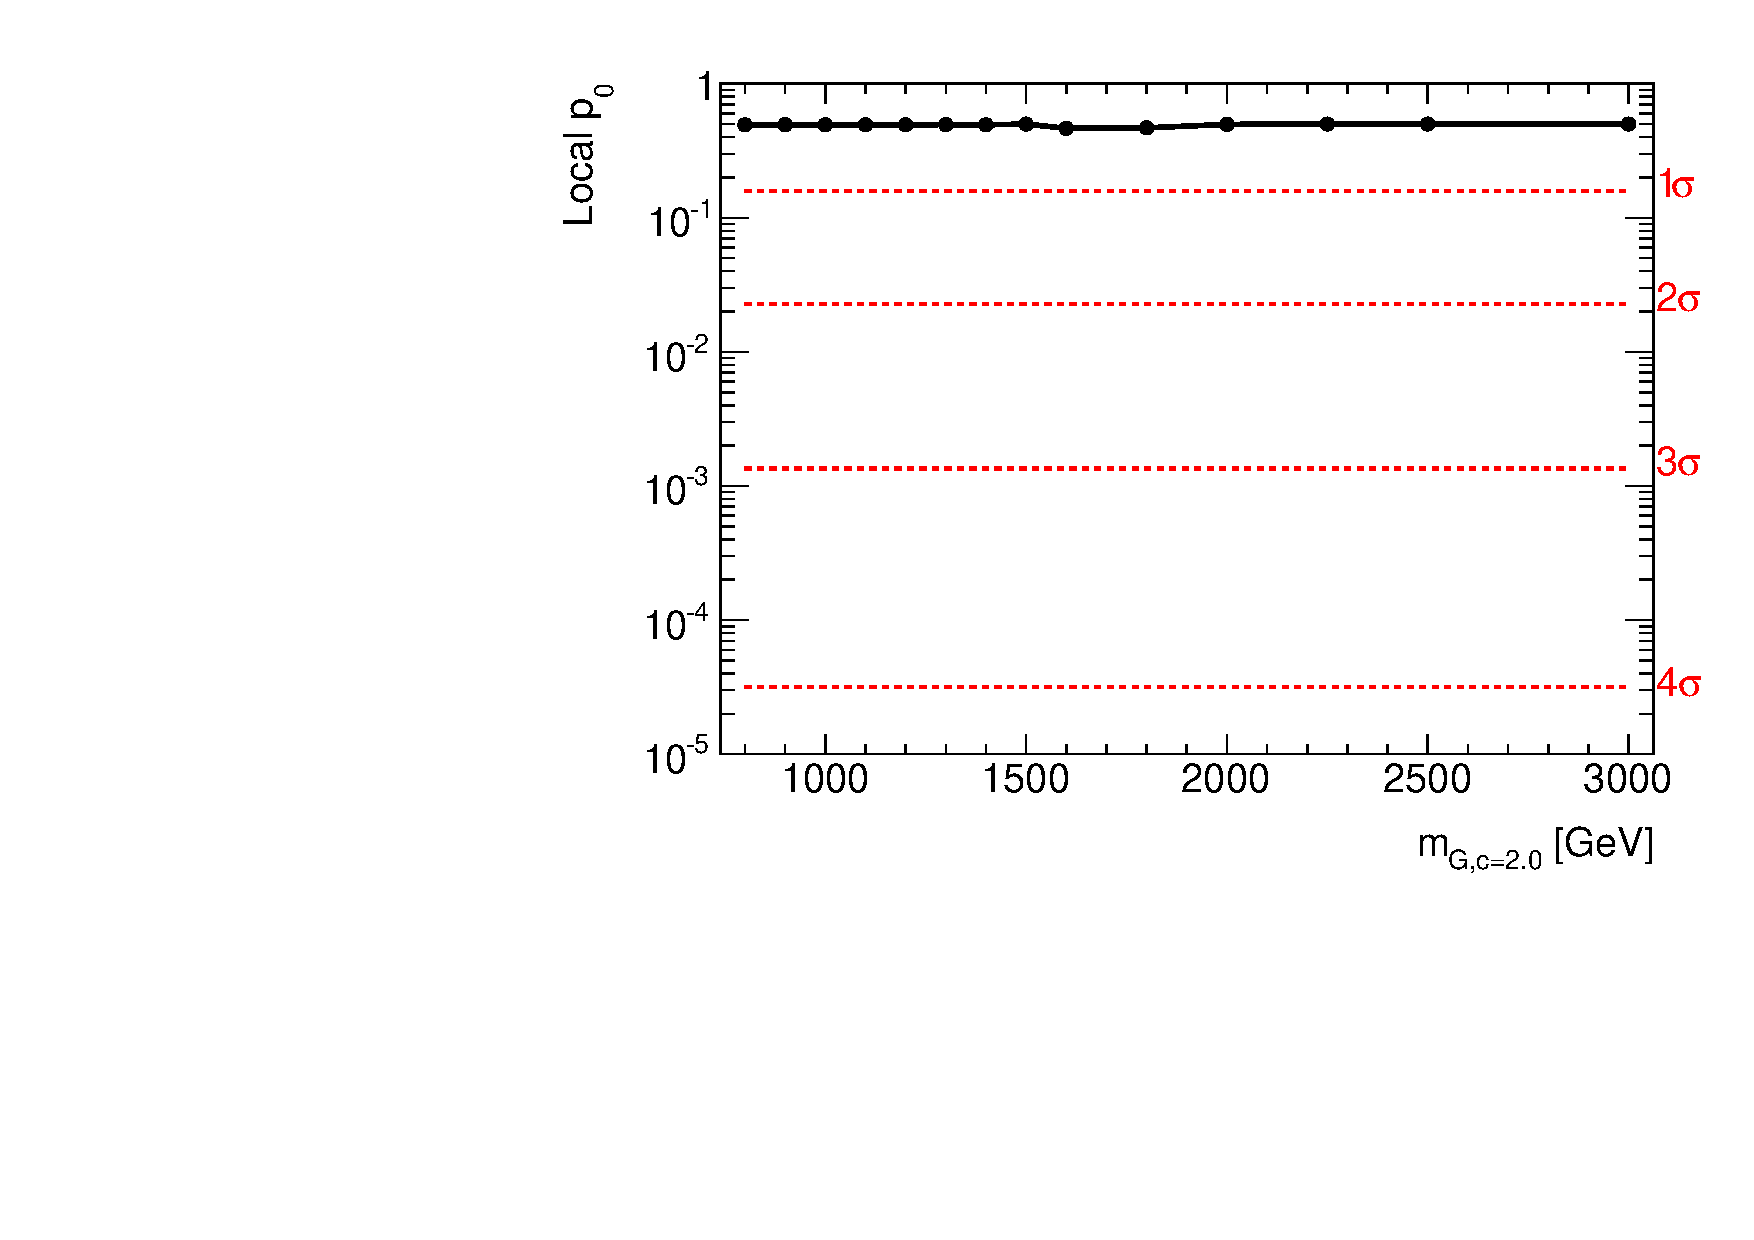
\includegraphics[width=\textwidth,angle=-90]{figures/boosted/results/p0_g20_allmasses_boosted.pdf}
        \caption{\Grav with $c=2$}
        \label{fig:localp0-g2}
    \end{subfigure}
  \caption{Local $p_0$ of the (a) scalar, (b) c=1 Graviton and (c) c=2 Graviton.}
  \label{fig:localp0}
\end{figure*}

\paragraph{}
Figure~\ref{fig:ranking2000} shows the pulls of the systematic uncertainty nuisance parameters and their correlations for the 2000 GeV mass point. 
The parameters are ranked by their post-fit impact. 
Only the leading 30 nuisance parameters are displayed.
One nuisance parameter (QCD\_ShapeCRHigh) in both the $2b$ and $3b$ samples shows a significant constraint coming from the signal region data. 
This nuisance parameter corresponds to the shape uncertainty on the QCD background derived from the $2b$ and $3b$ control regions, as explained in Section \ref{unc-shape-qcd-in-sr}. 
The prior probability distributions for this nuisance parameter is very broad.
The relative uncertainty on the background prediction is extremely high at high \mtwoJ. 
This is because there is very little data in the control region at high mass to constrain this uncertainty.

\begin{figure*}[htb!]
\centering
\captionsetup{justification=centering}
    \begin{subfigure}[b]{0.31\textwidth}
        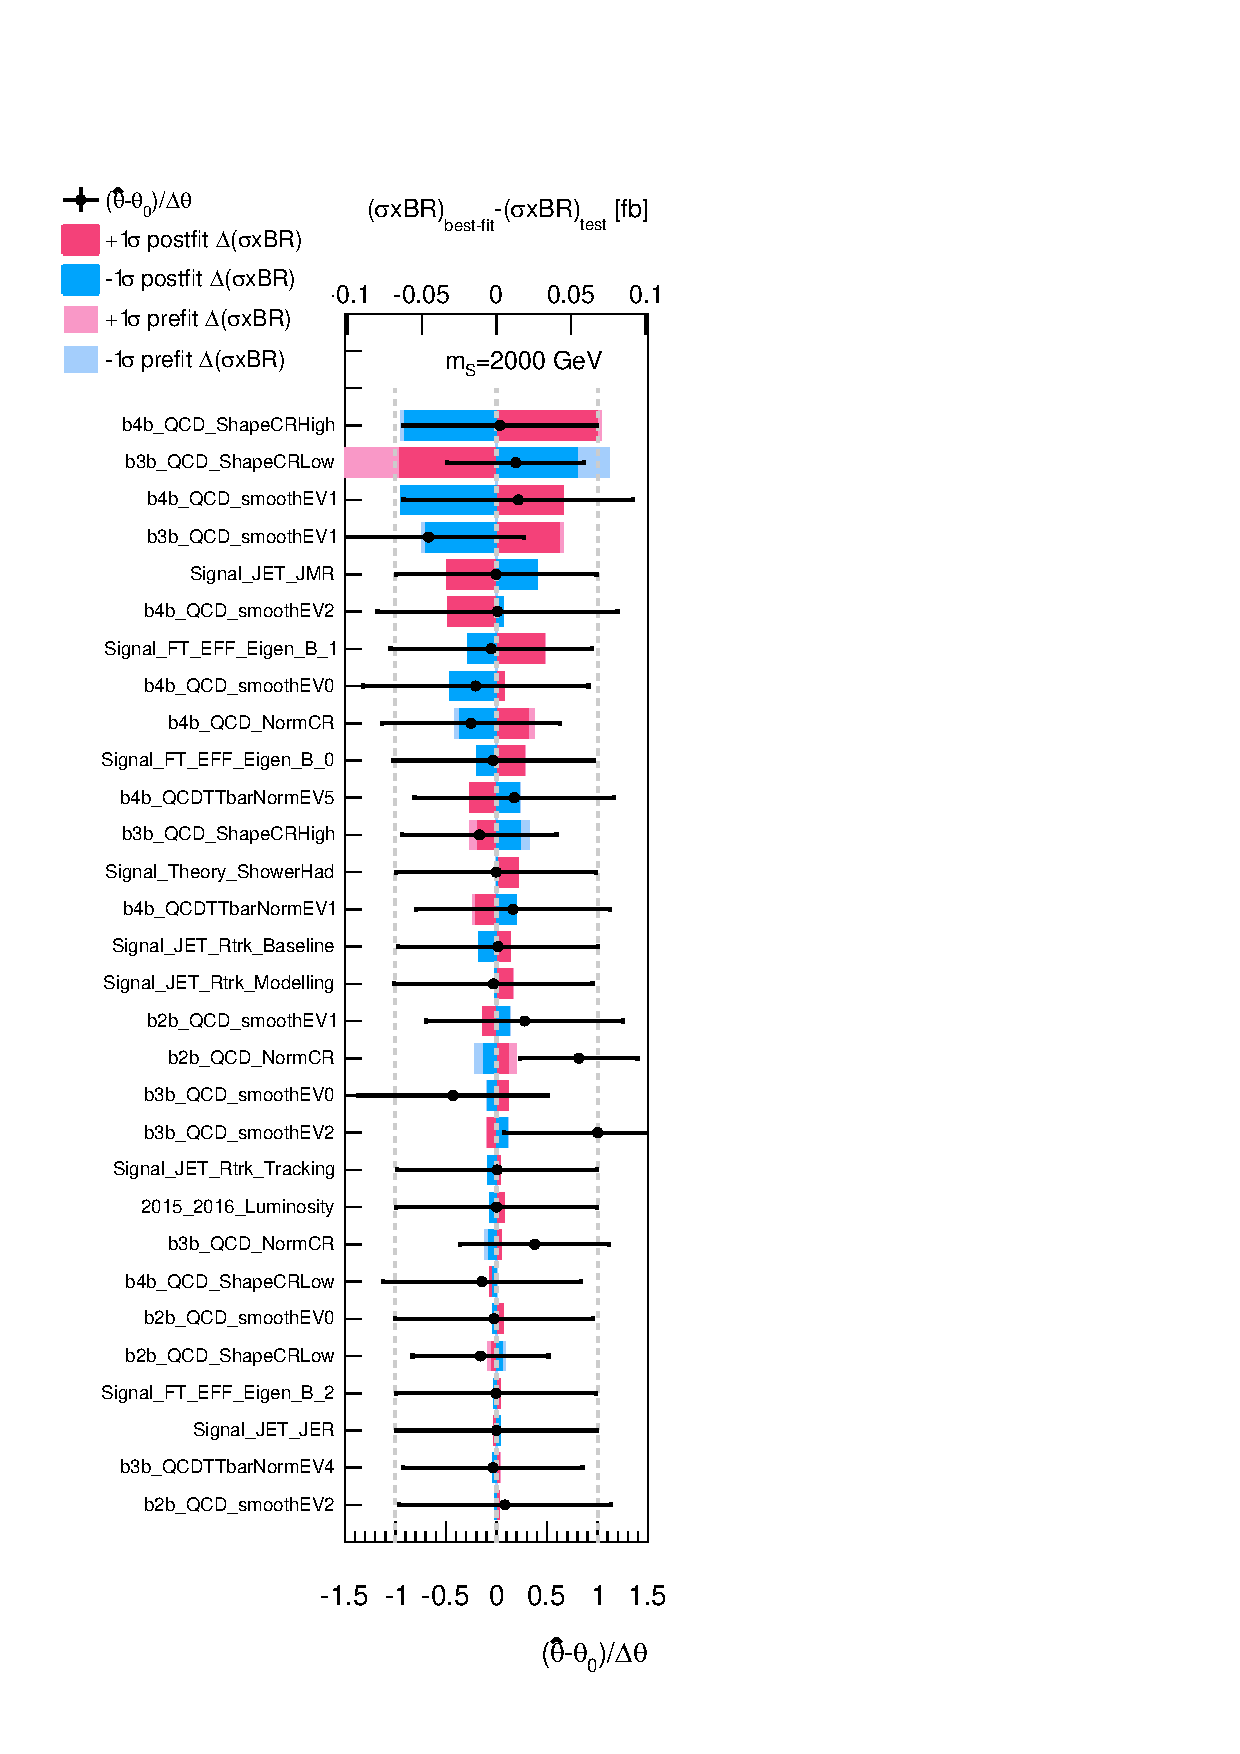
\includegraphics[width=\textwidth]{figures/boosted/results/ranking_okt18_s_2000.pdf}
        \caption{scalar}
        \label{fig:ranking2000-s}
    \end{subfigure}
    \quad 
    \begin{subfigure}[b]{0.31\textwidth}
        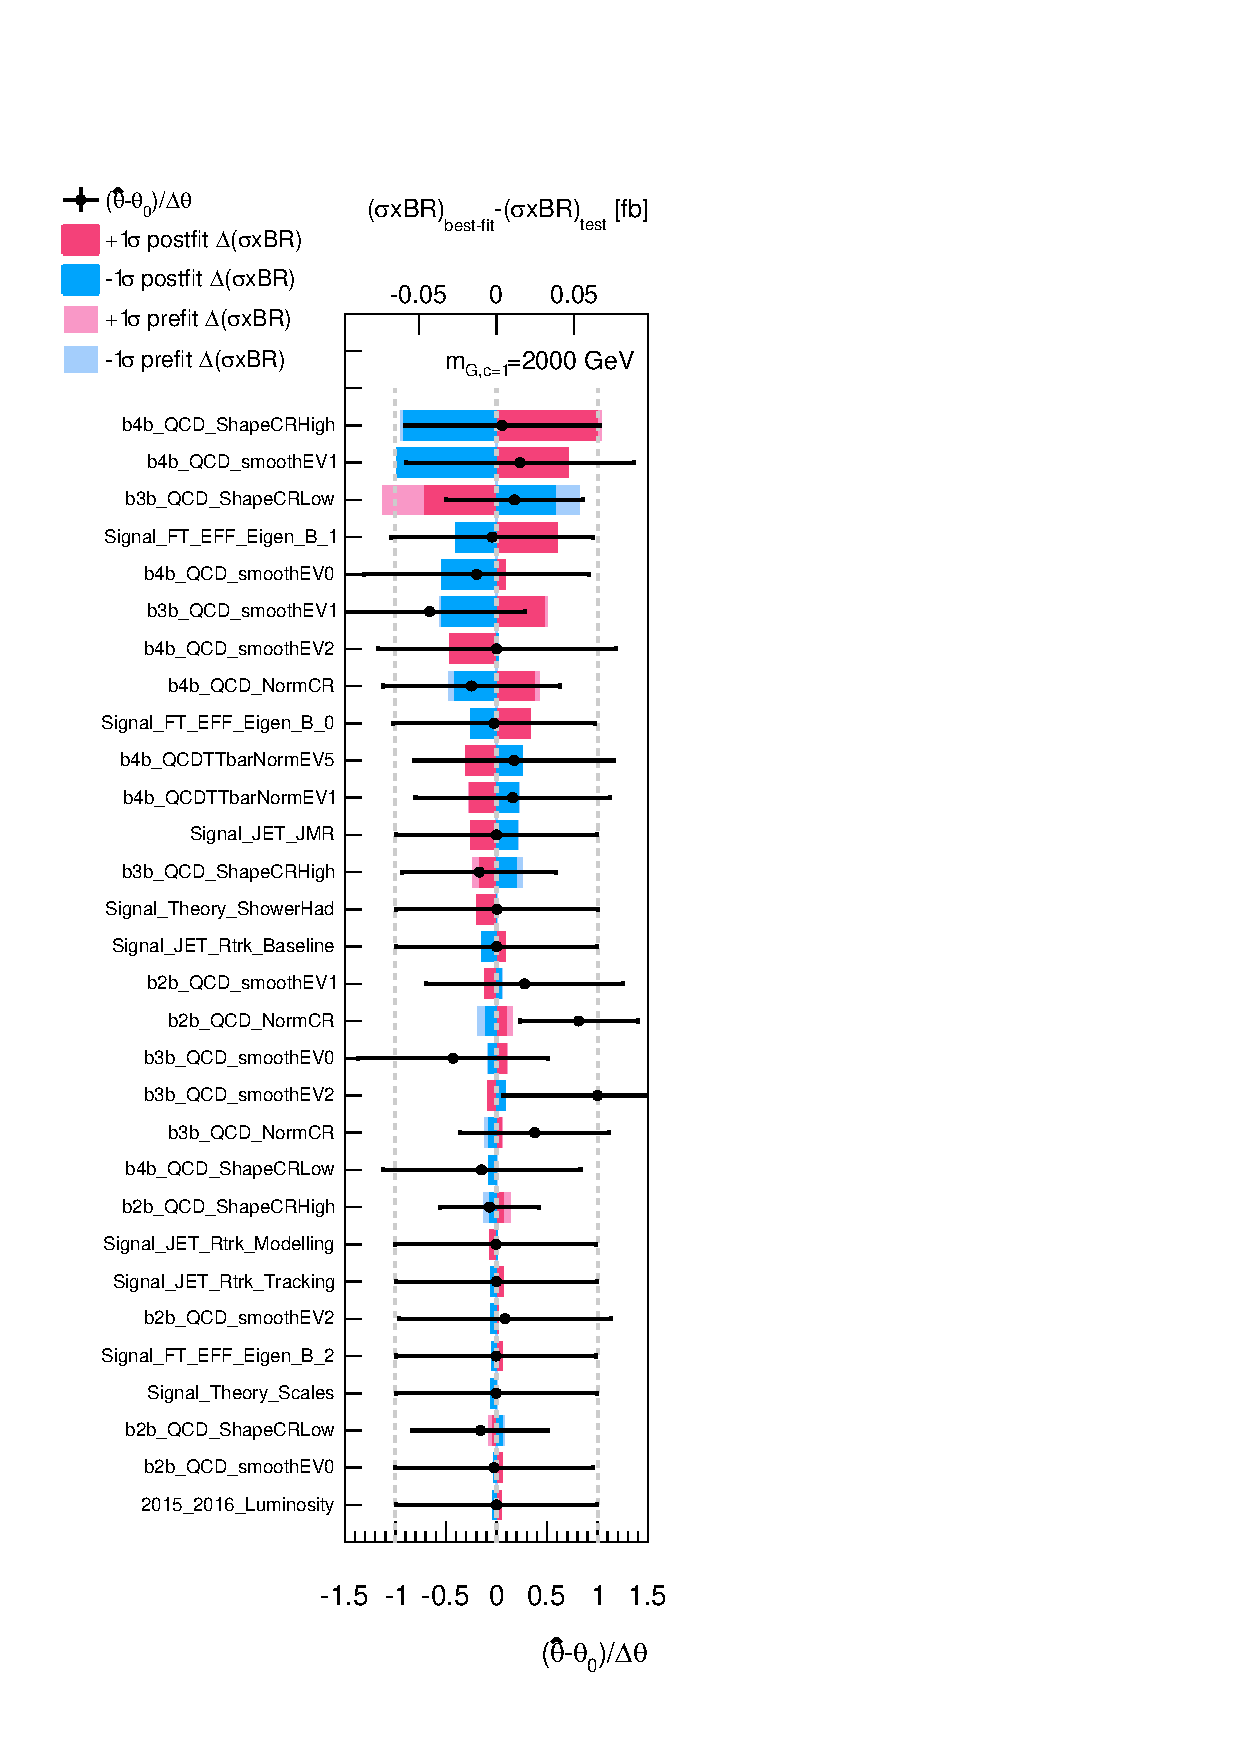
\includegraphics[width=\textwidth]{figures/boosted/results/ranking_okt18_g10_2000.pdf}
        \caption{\Grav with $c=1$}
        \label{fig:ranking2000-g1}
    \end{subfigure}
    \quad
    \begin{subfigure}[b]{0.31\textwidth}
        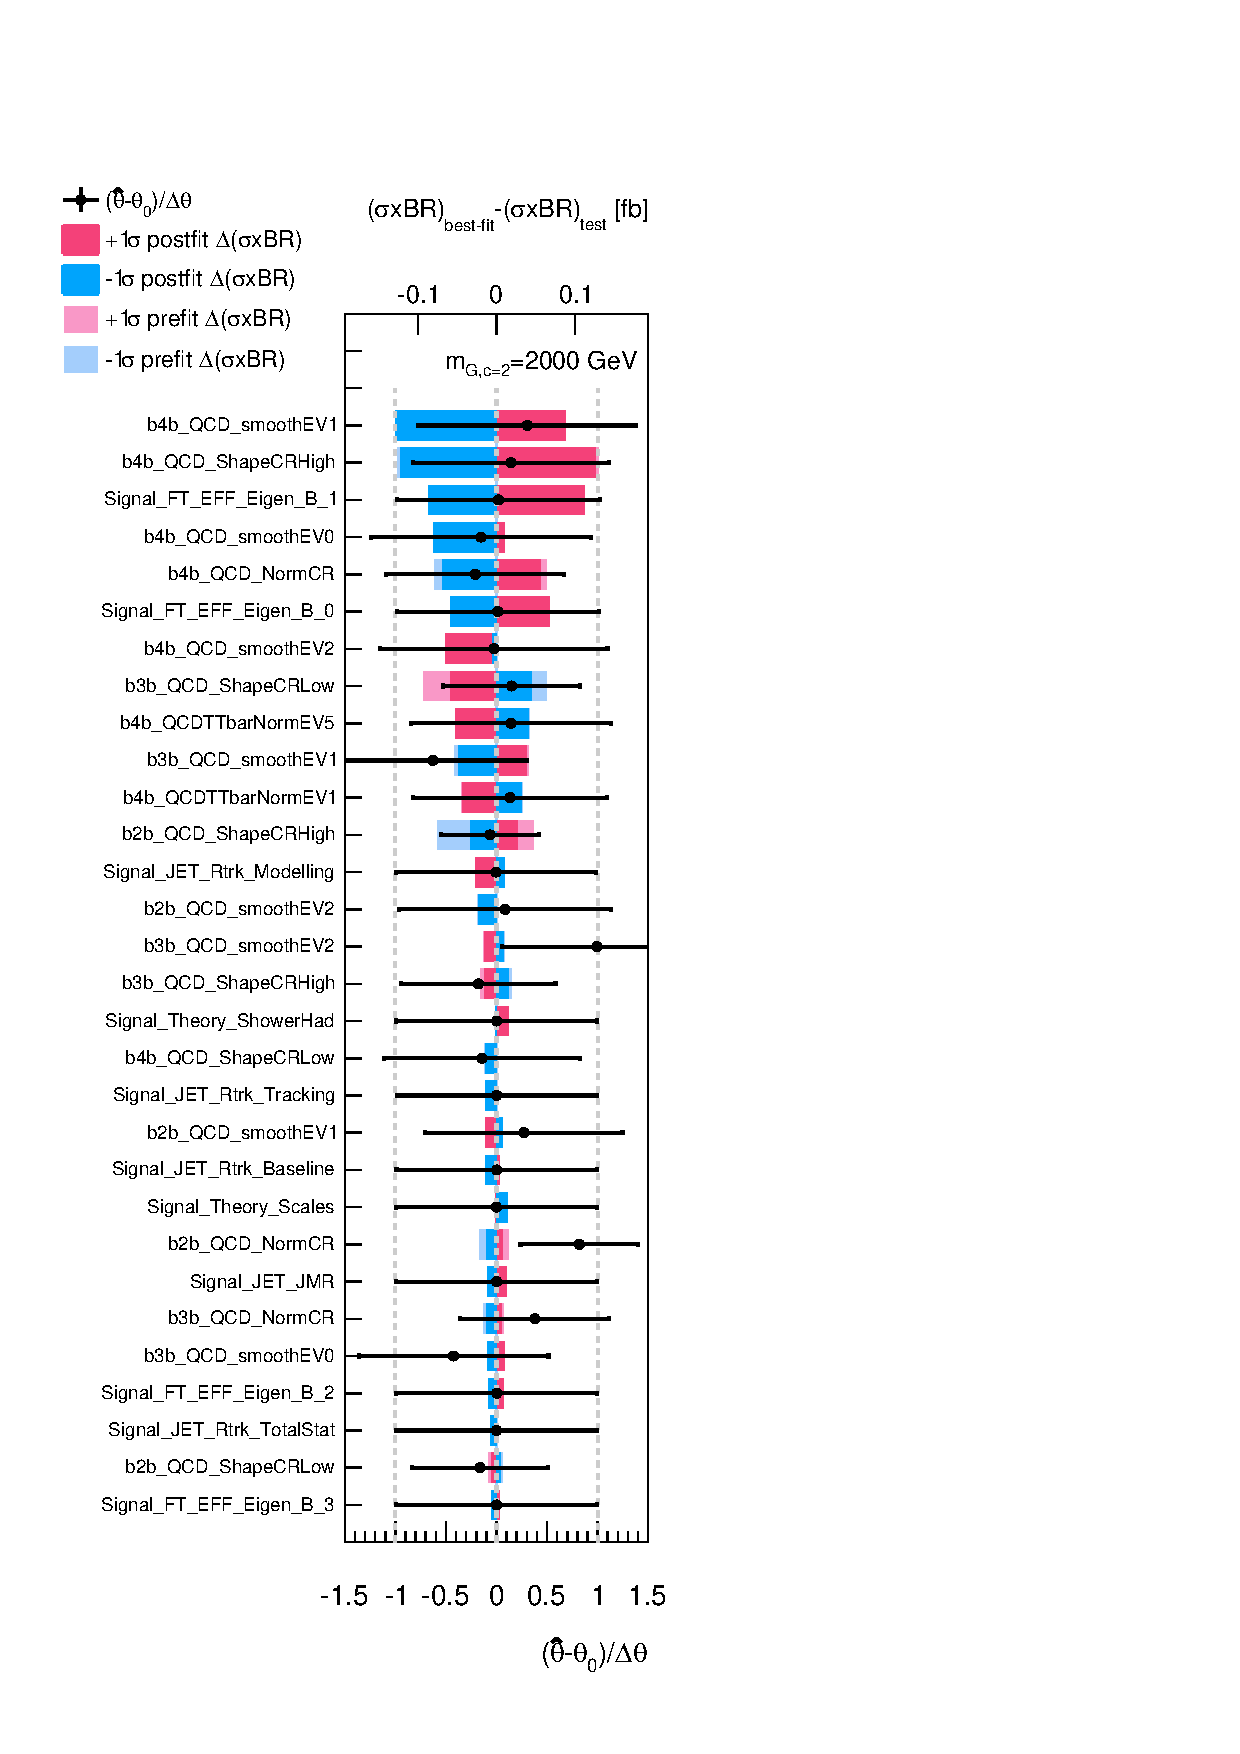
\includegraphics[width=\textwidth]{figures/boosted/results/ranking_okt18_g20_2000.pdf}
        \caption{\Grav with $c=2$}
        \label{fig:ranking2000-g2}
    \end{subfigure}
  \caption{The impact of nuisance parameters on the fitted cross section, ranked by their post-fit impact. The signal mass used in this fits is 2000~GeV, and the signal model is (a) narrow scalar, (b) \Grav~ with $c=1$ and (c) \Grav~ with $c=2$.}
  \label{fig:ranking2000}
\end{figure*}


\paragraph{}
Examples of the fit used to set these limits are shown in Figures~\ref{fig:postfit2000}, where a narrow-width scalar $H$ is used for the signal model. 
In cases where the best-fit is negative, the fit is repeated with $\mu$ bounded to zero. 
At $2$ \TeV, the fitted signal is positive ($\mu=0.1\pm0.25$) though well consistent with the background-only hypothesis. 
In all fits, good agreement is seen between data and the background only model.

\begin{figure}[htb!]
\centering
\captionsetup{justification=centering}
    \hspace{-2cm}
    \begin{subfigure}[b]{0.33\textwidth}
        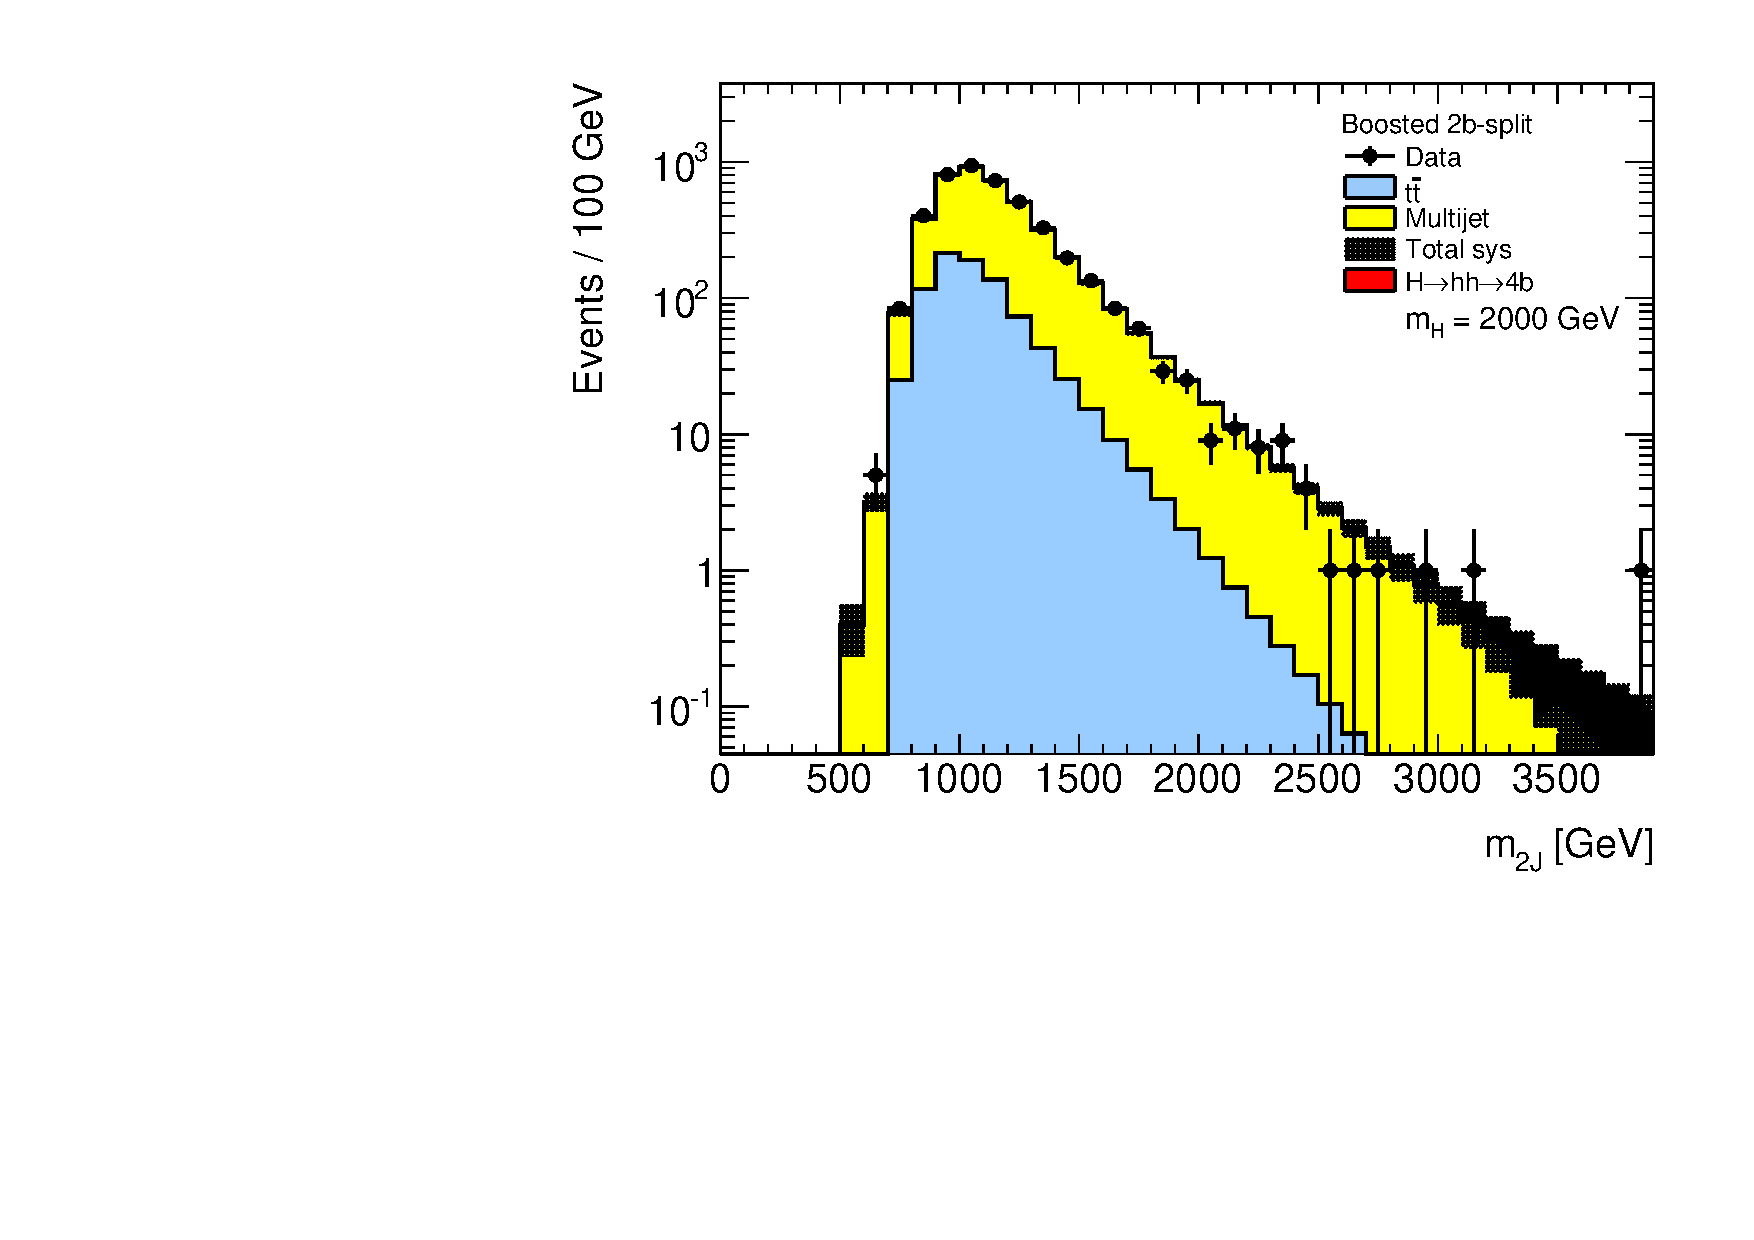
\includegraphics[width=\textwidth,angle=-90]{figures/boosted/results/postfitplot_s_2000_b2b.pdf}
        \caption{$2bs$ post-fit}
        \label{fig:postfit2bs}
    \end{subfigure}
    \quad \quad \quad \quad
    \begin{subfigure}[b]{0.33\textwidth}
        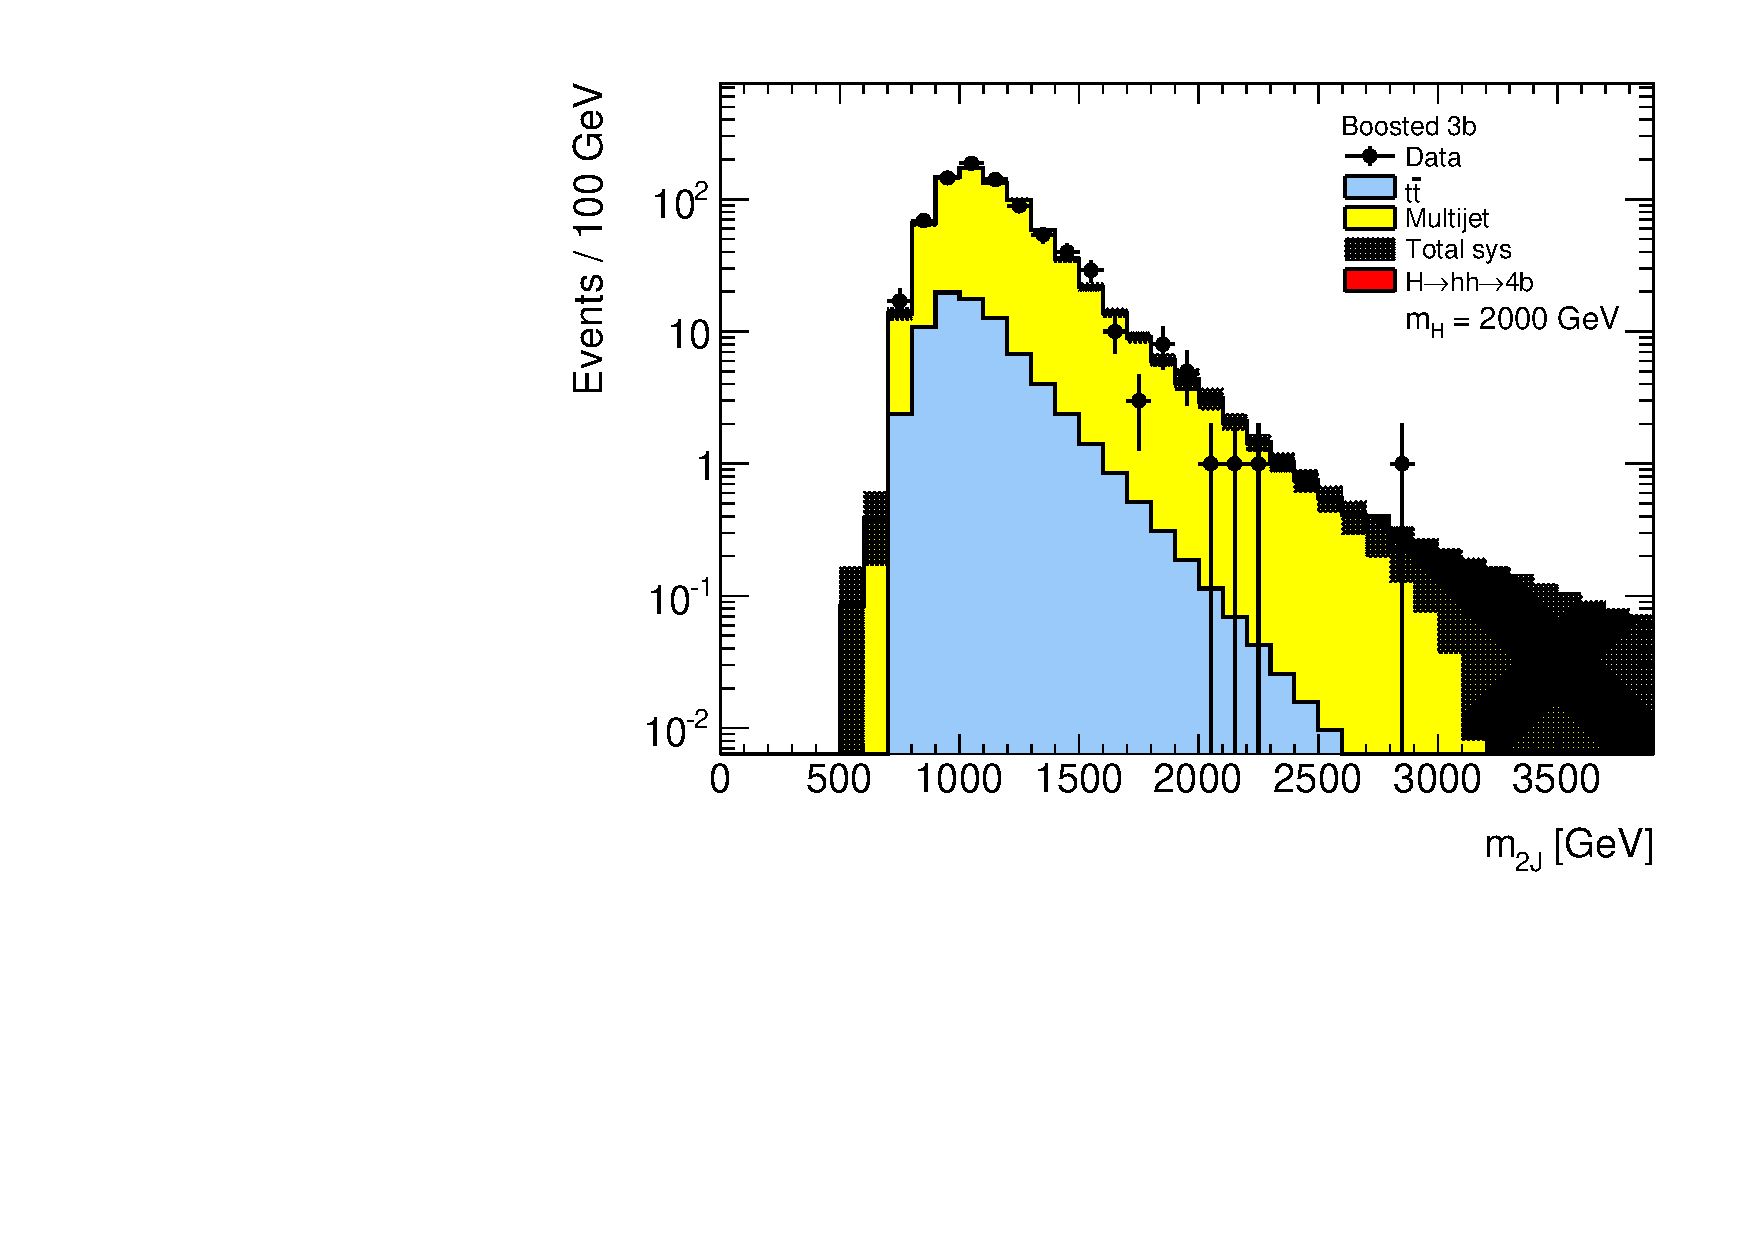
\includegraphics[width=\textwidth,angle=-90]{figures/boosted/results/postfitplot_s_2000_b3b.pdf}
        \caption{$3b$ post-fit}
        \label{fig:postfit3b}
    \end{subfigure}
    \\
    \begin{subfigure}[b]{0.33\textwidth}
        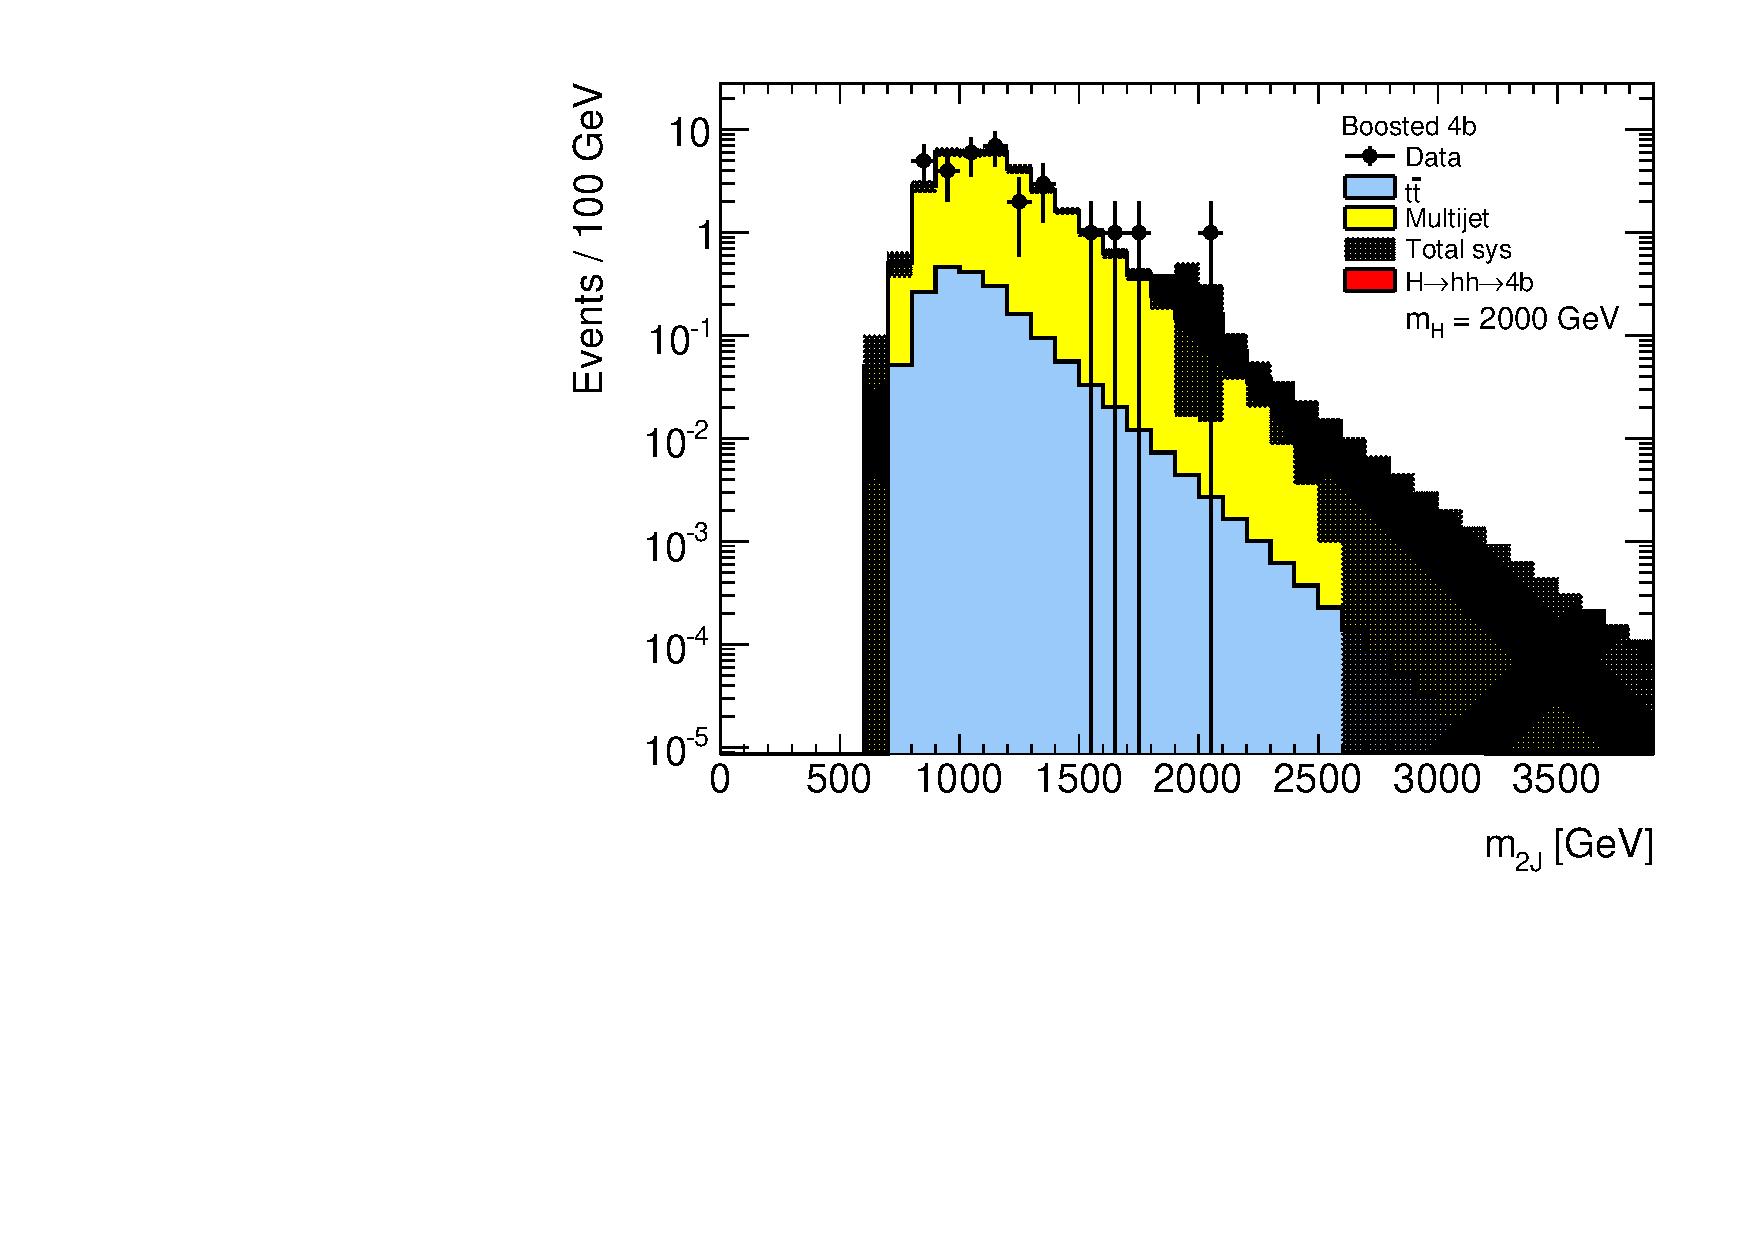
\includegraphics[width=\textwidth,angle=-90]{figures/boosted/results/postfitplot_s_2000_b4b.pdf}
        \caption{$4b$ post-fit}
        \label{fig:postfit4b}
    \end{subfigure}
\caption{Post-fit signal region scaled \mtwoJ~ distributions after fitting the data with the $2$ \TeV~ \Grav~ with $c=1.0$ hypothesis. The signal strength is slightly positive.}
\label{fig:postfit2000}
\end{figure}

\paragraph{}
The observed limit for the narrow scalar and \Grav is shown in Figure~\ref{fig:limit_boosted_g10},~\ref{fig:limit_boosted_g20}, and~\ref{fig:limit_boosted_scalar}.
The stat-only limit is also shown. The impact of systematic uncertainties is small. 
These limits do not contain any input from the resolved analysis.

\begin{figure*}
\begin{center}
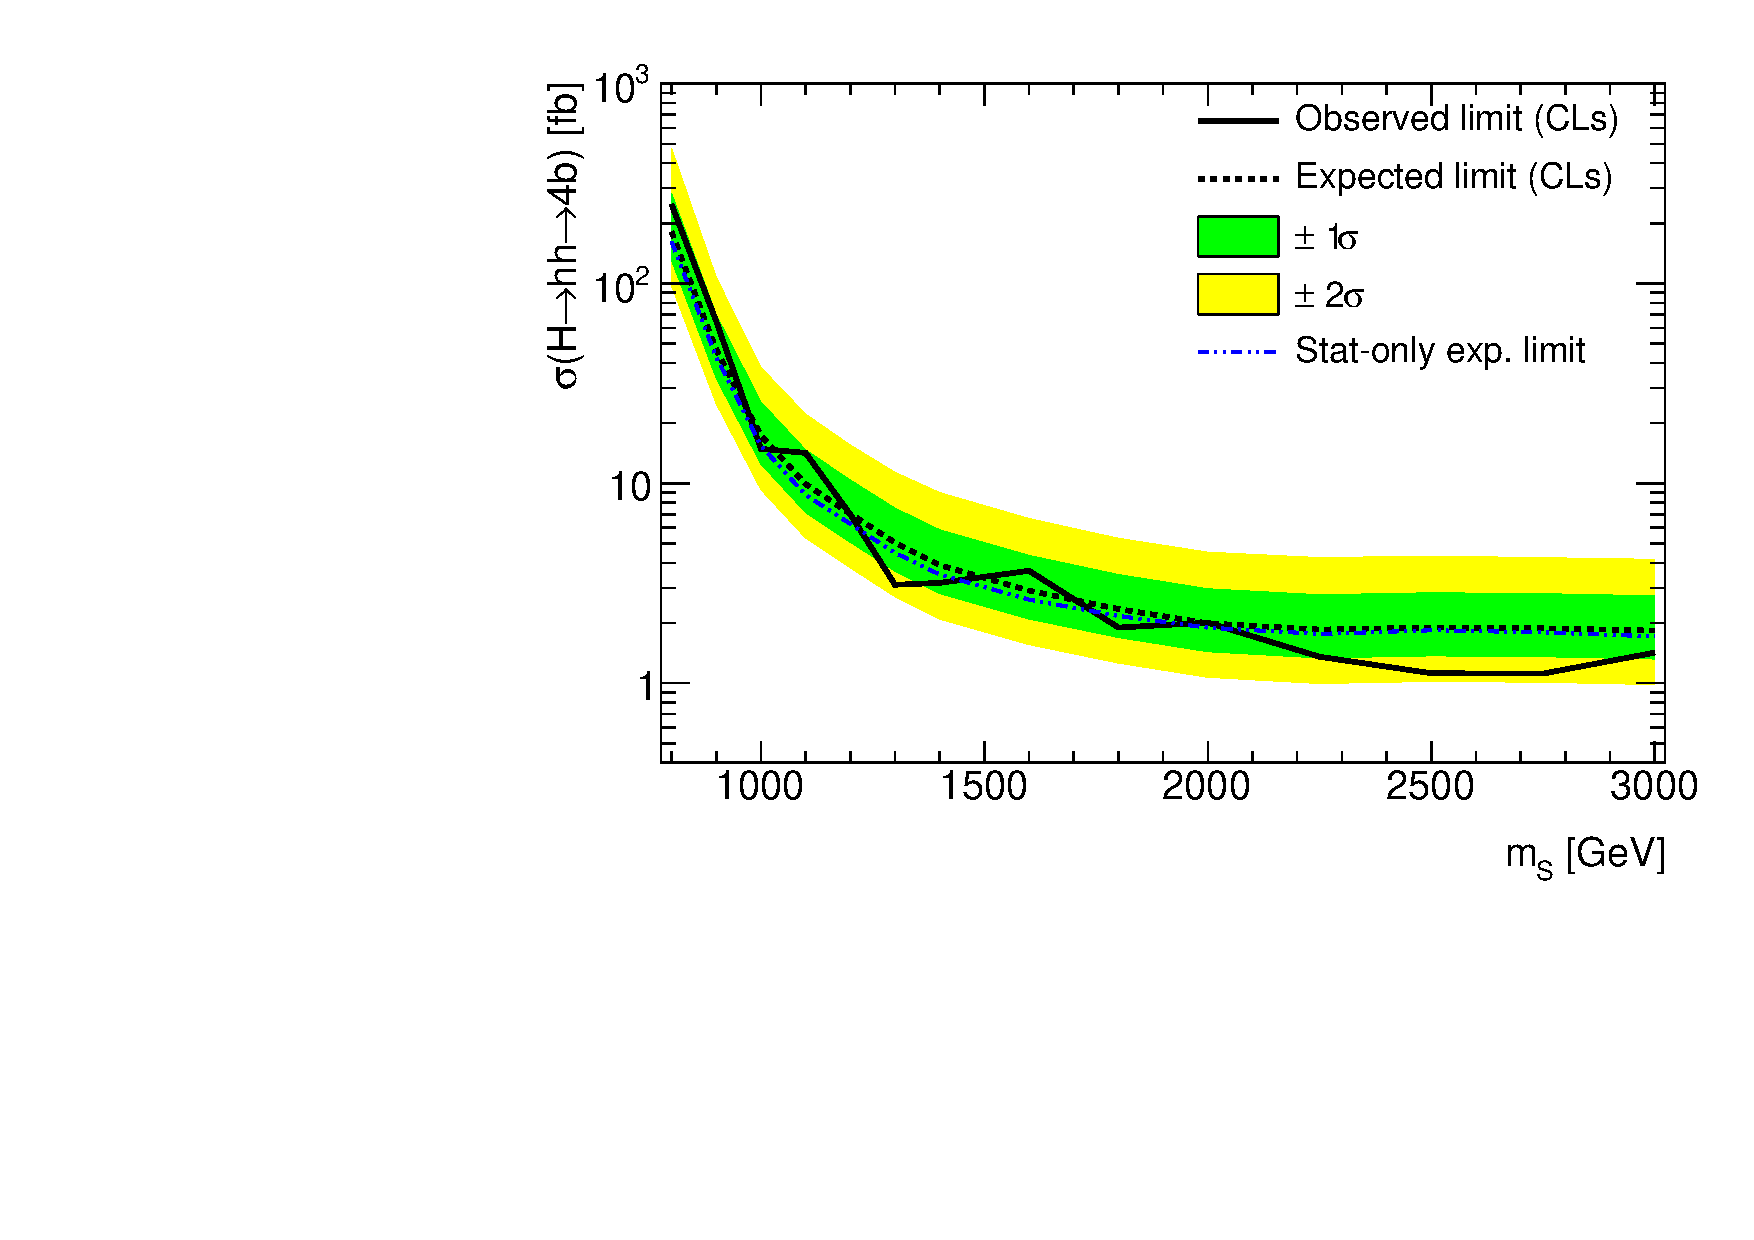
\includegraphics[width=0.4\textwidth,angle=-90]{figures/boosted/results/limit_boosted_boosted_okt18_s.pdf}
\caption{The expected and observed $95\%$ CL upper exclusion limits for the boosted analysis calculated including all systematic uncertainties for the narrow scalar model. The dot-dashed line shows the expected limit when only statistical uncertainties are included. The limits are derived with the asymptotic approximation.}
\label{fig:limit_boosted_g10}
\end{center}
\end{figure*}

\begin{figure*}
\begin{center}
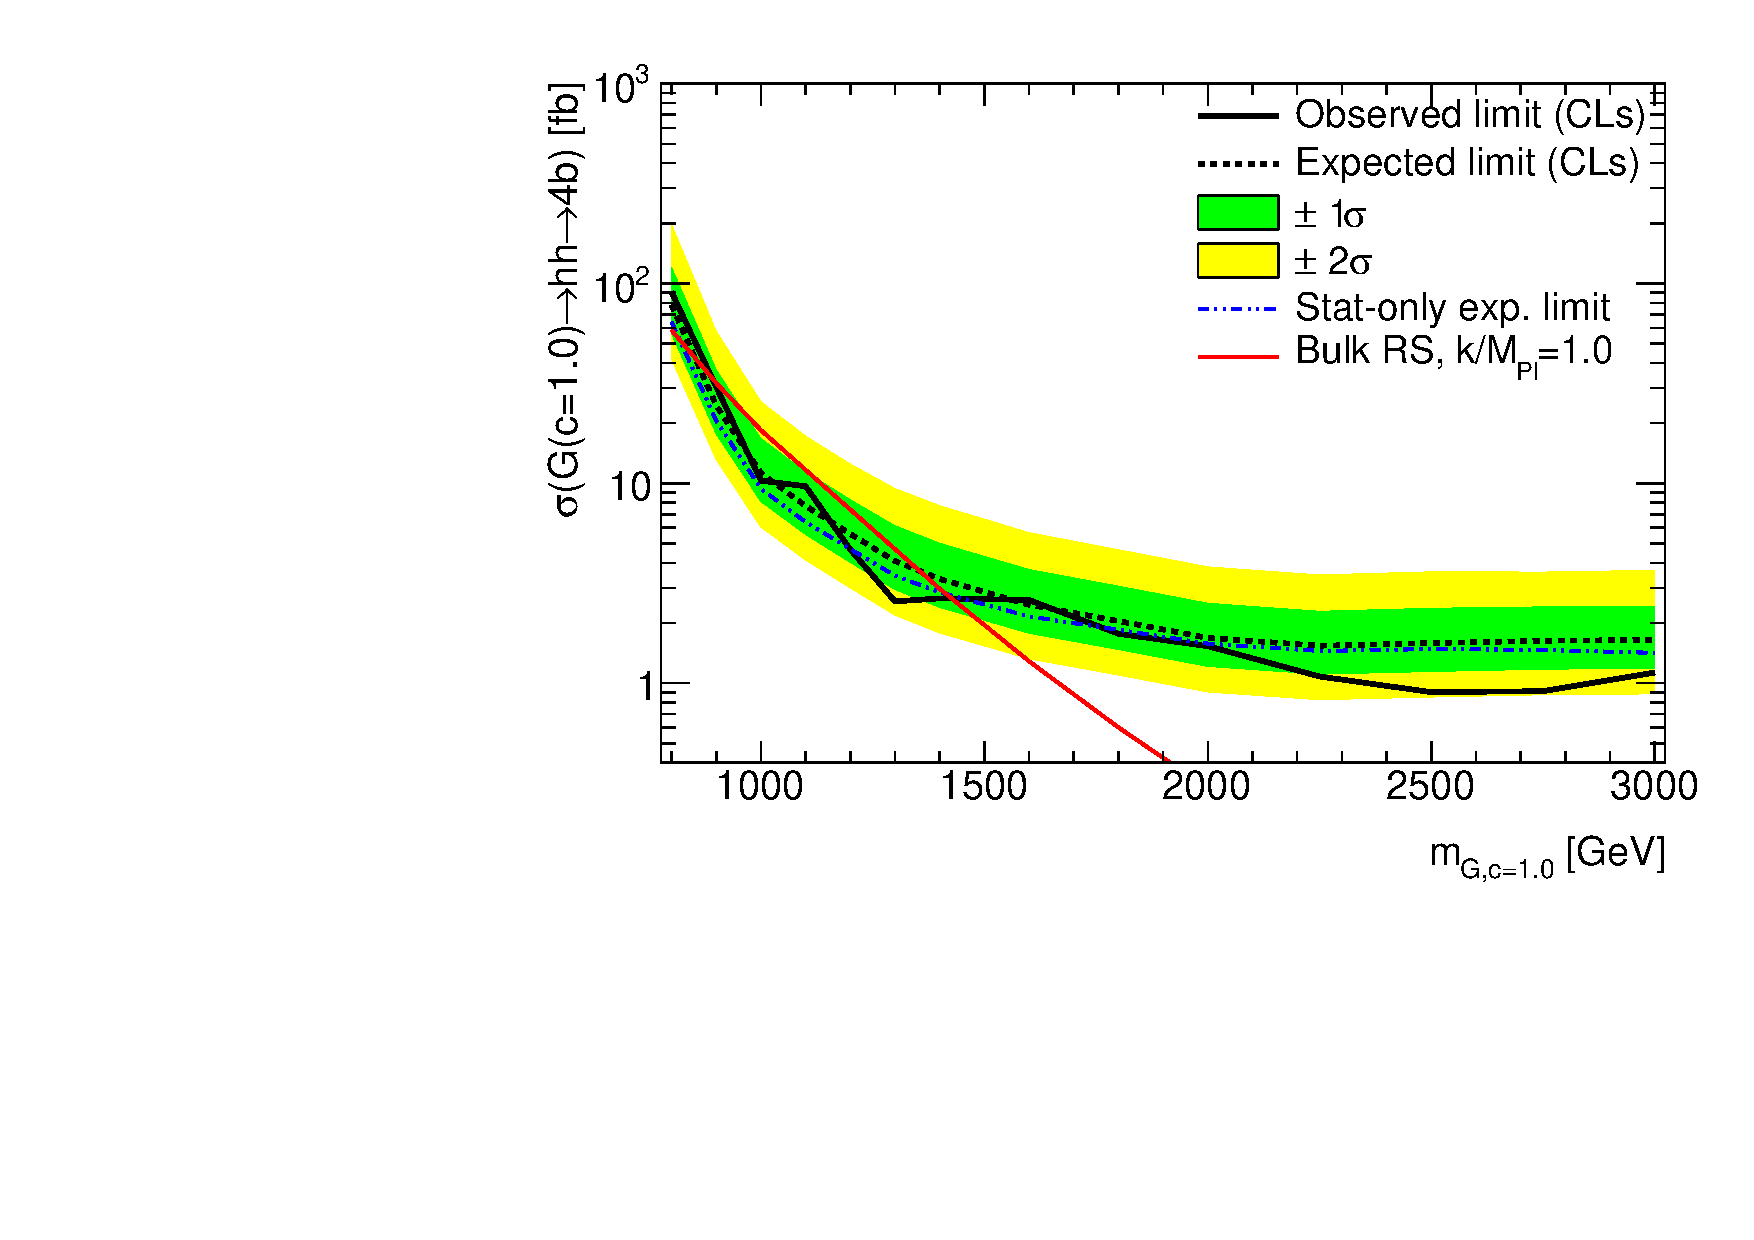
\includegraphics[width=0.4\textwidth,angle=-90]{figures/boosted/results/limit_boosted_boosted_okt18_g10.pdf}
\caption{The expected and observed $95\%$ CL upper exclusion limits for the boosted analysis calculated including all systematic uncertainties for the $c=1.0$ Graviton. The dot-dashed line shows the expected limit when only statistical uncertainties are included. The limits are derived with the asymptotic approximation.}
\label{fig:limit_boosted_g20}
\end{center}
\end{figure*}
\begin{figure*}

\begin{center}
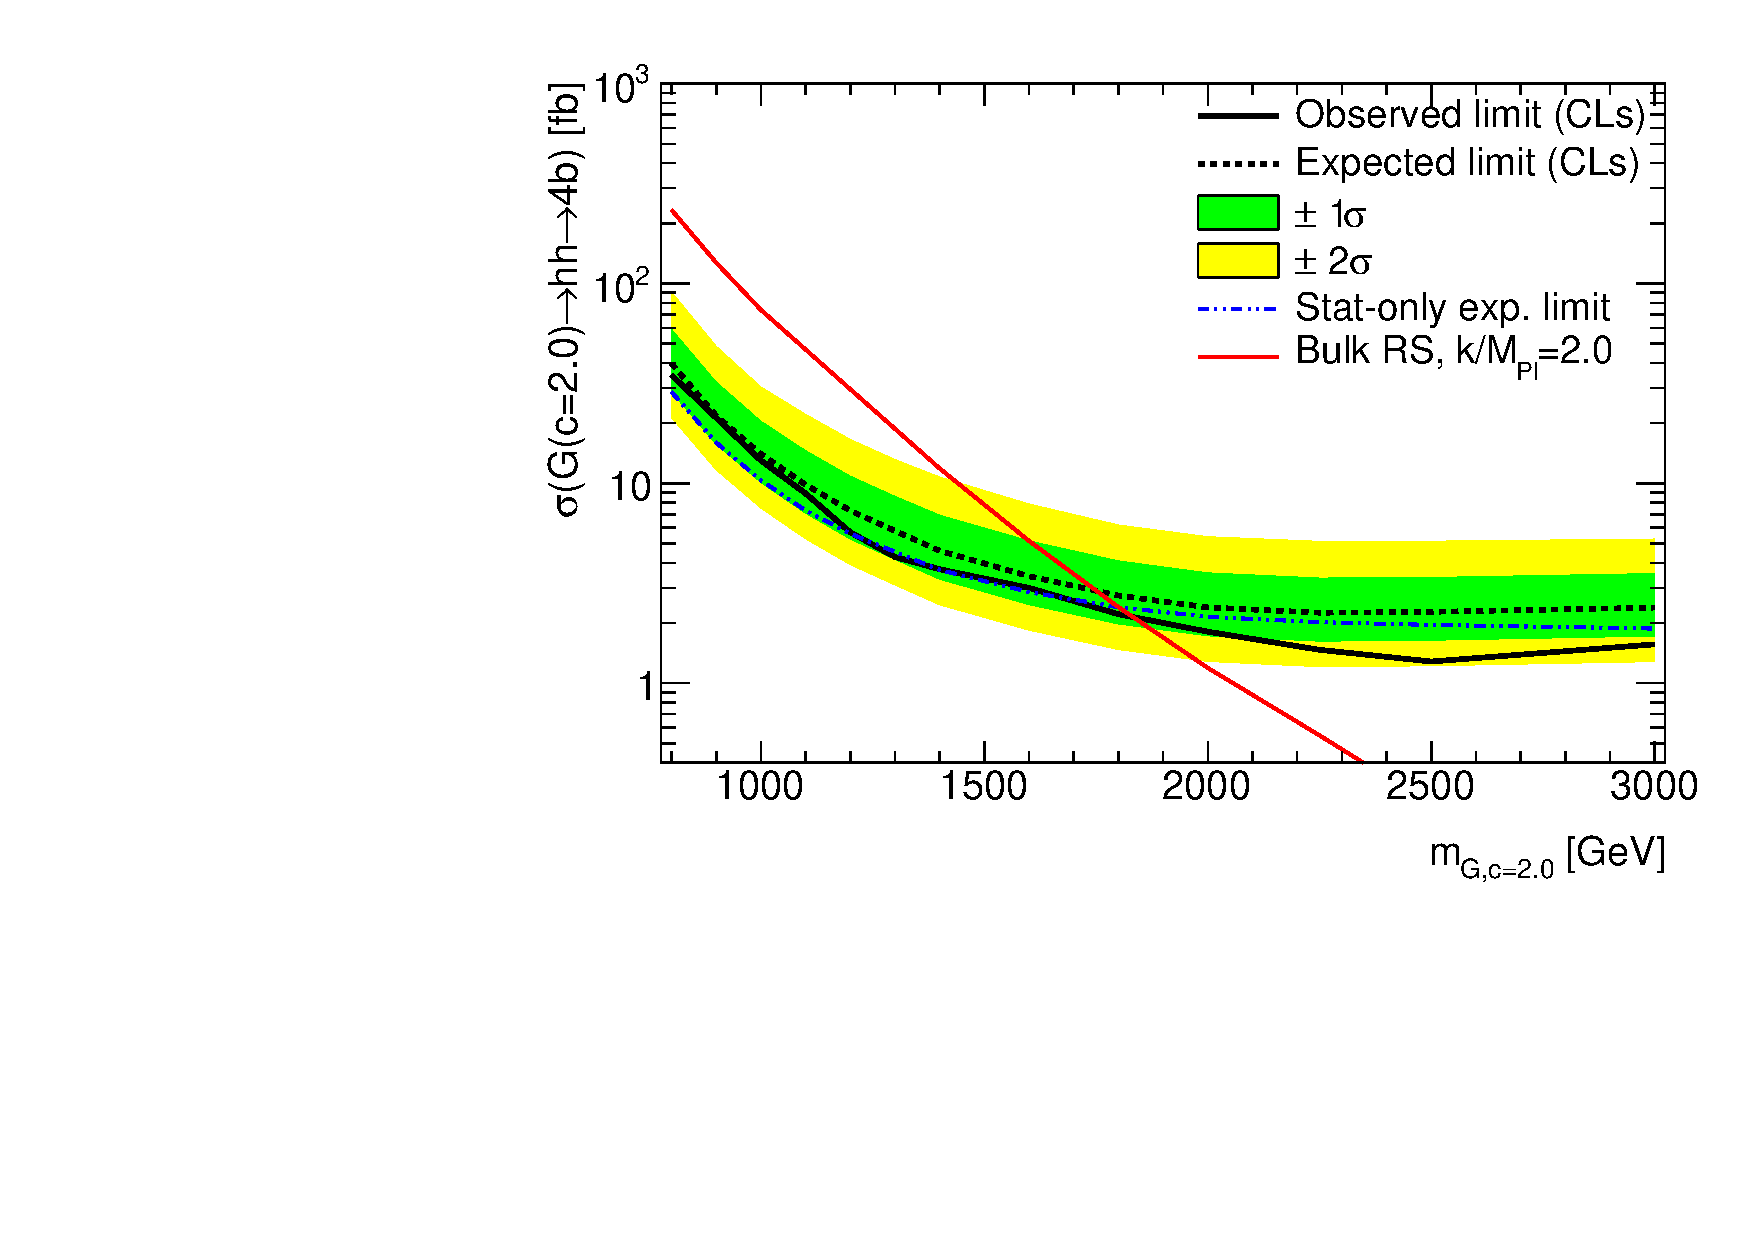
\includegraphics[width=0.4\textwidth,angle=-90]{figures/boosted/results/limit_boosted_boosted_okt18_g20.pdf}
\caption{The expected and observed $95\%$ CL upper exclusion limits for the boosted analysis calculated including all systematic uncertainties for the $c=2.0$ Graviton. The dot-dashed line shows the expected limit when only statistical uncertainties are included. The limits are derived with the asymptotic approximation.}
\label{fig:limit_boosted_scalar}
\end{center}
\end{figure*}


\section{Boosted and resolved combined limits}
\label{sec:combinedlimits}
\paragraph{}
The observed limit for the narrow scalar is shown in Figure~\ref{fig:limit_scalar}.
The observed limits for the Graviton models is shown in Figure~\ref{fig:limit_g10} for $c = 1$ and in Figure~\ref{fig:limit_g20} for $c = 2$.
The bulk RS model with $c = 1$ is excluded for masses between $313$ and $1362$~\GeV, and the bulk RS model with $c = 2$ is excluded for masses below $1744$~\GeV. 
In the heavy Higgs model, the cross section upper limits for $\sigma(pp \to H \to hh \to b\bar{b}b\bar{b})$ range from $1$ to $10$ fb in the mass range of $1000$ to $3000$ \GeV.

\paragraph{}
From Figure~\ref{fig:limit_scalar}, different expected exclusion limits from the analysis can be compared.
The resolved analysis is only sensitive to resonance searches up to $900$ \GeV.
The boosted $4b$ is most sensitive for resonances between $1200$ and $1800$ \GeV.
The boosted $3b$ is most sensitive for resonances between $2000$ and $2500$ \GeV.
The boosted $2bs$ is most sensitive for resonances between $2500$ and $3000$ \GeV.
The combination significantly improves the sensitivity between $1$ and $1.5$ \TeV~ for resonant signals.                                                                                
The result is limited by systematic uncertainties in the background normalization and shape.
Since these are data-driven, an increase of the integrated luminosity will improve the sensitivity.

\paragraph{}
The non-resonant search is performed using the resolved analysis only, since it has much better sensitivity to non-resonant signals than the boosted analysis. 
Using the SM di-Higgs non-resonant production via gluon--gluon fusion as the signal model, and applying the NNLO and finite top-quark mass correction, the observed 95\% CL upper limit is $\sigma(pp\rightarrow hh \rightarrow b\bar{b}b\bar{b}) < 147$ fb. 
The expected and observed limit values and the uncertainties in the expectation are given in Table~\ref{tab:smrwMhhlims}.
The observed limit is stronger than the expected due to the slight deficit of events in \mfourj~ around $500-600$ \GeV.

\begin{table}[htp]
\caption{95\% CL exclusion limits for SM non-resonant di-Higgs production, in units of the SM prediction for ${\sigma(pp\rightarrow hh \rightarrow b\bar{b}b\bar{b})}$.}
\begin{center}
\begin{tabular}{cccccc}
\toprule
Observed & $-2\sigma$ & $-1\sigma$ & Expected & $+1\sigma$ & $+2\sigma$ \\
\midrule
13.0 & 11.1 & 14.9 & 20.7 & 30.0 & 43.5 \\
\bottomrule
\label{tab:smrwMhhlims}
\end{tabular}
\end{center}
\end{table}

\begin{figure*}
\begin{center}
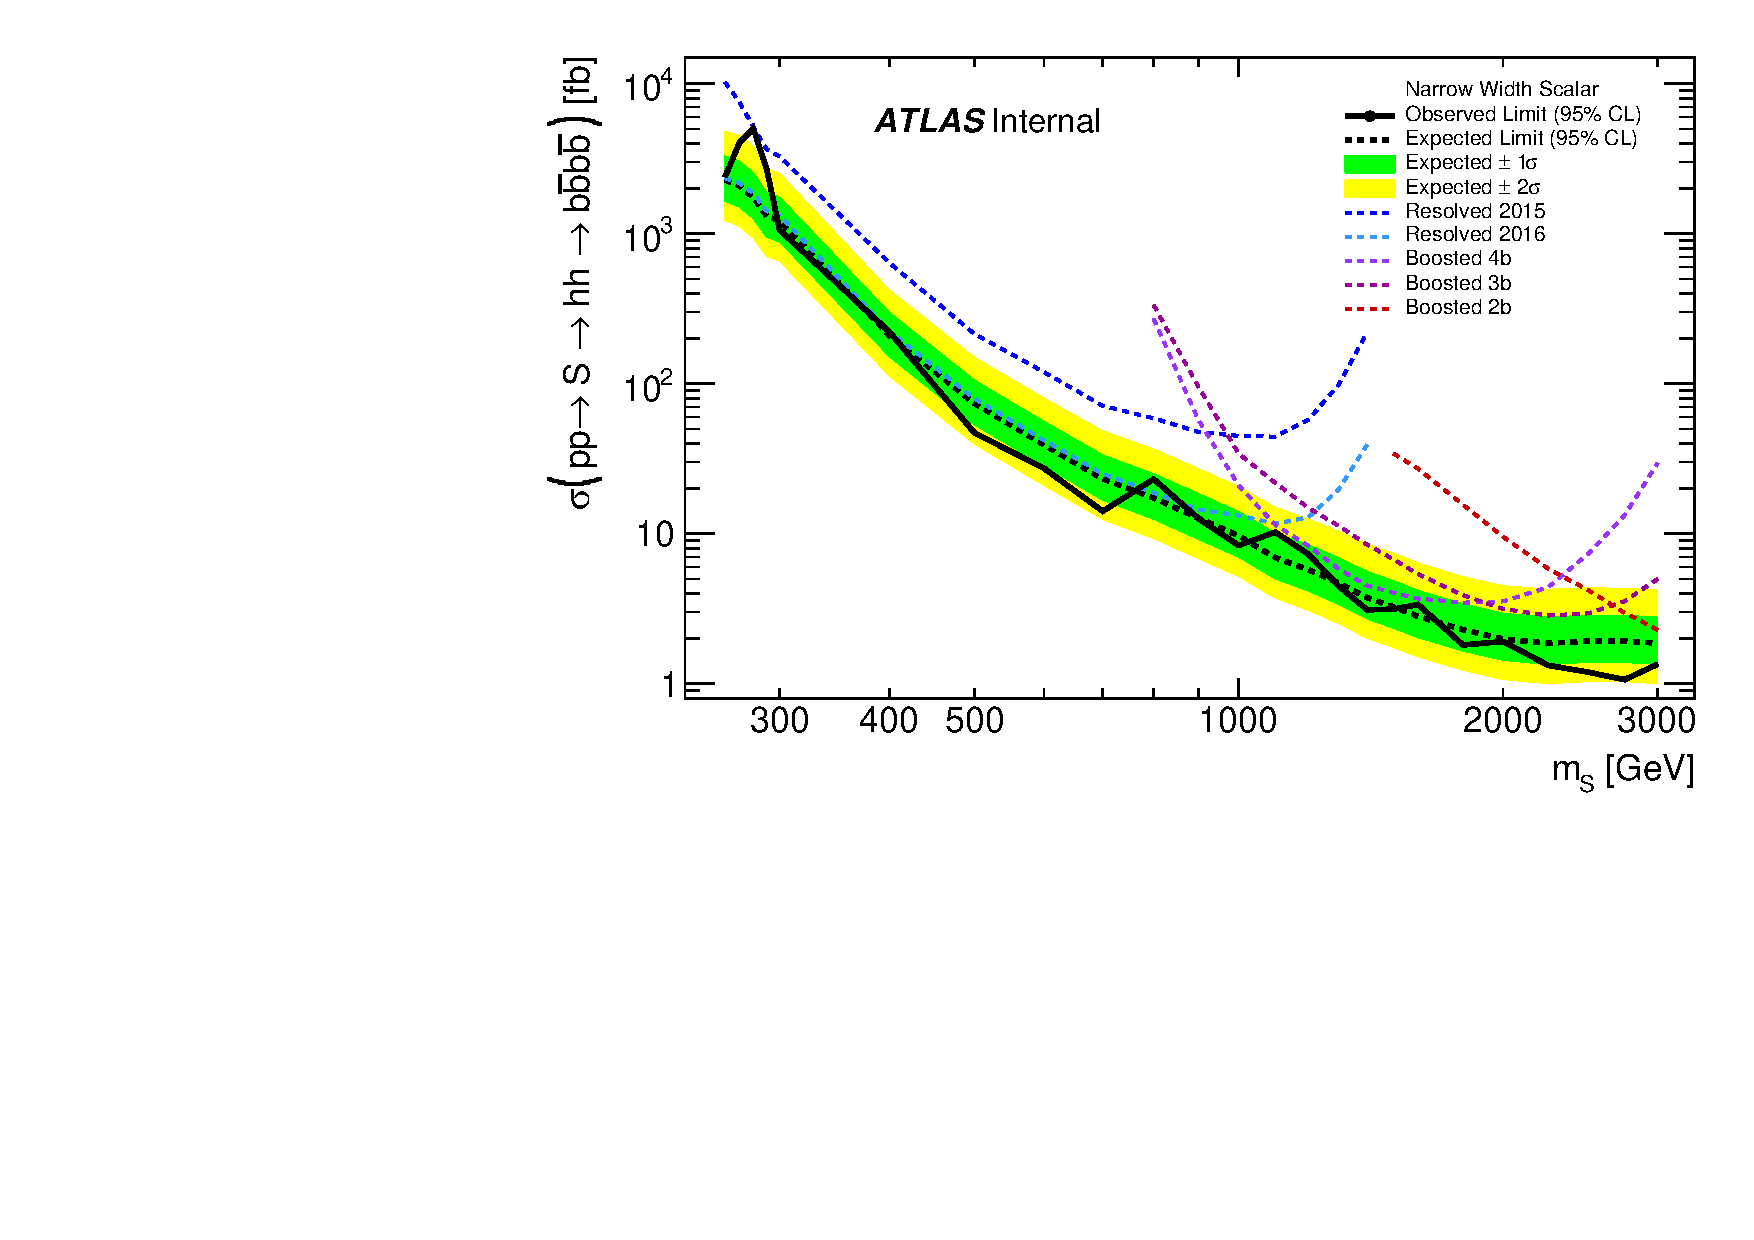
\includegraphics[width=0.4\textwidth,angle=-90]{figures/boosted/results/BrazilPlot_Asymptotic_s_hh_combined_AllSyst_unblinded_2017-10-04.pdf}
\caption{The expected and observed $95\%$ CL upper exclusion limits for the combined analysis calculated including all systematic uncertainties for the narrow scalar model. The dot-dashed line shows the expected limit when only statistical uncertainties are included. The limits are derived with the asymptotic approximation.}
\label{fig:limit_g10}
\end{center}
\end{figure*}

\begin{figure*}
\begin{center}
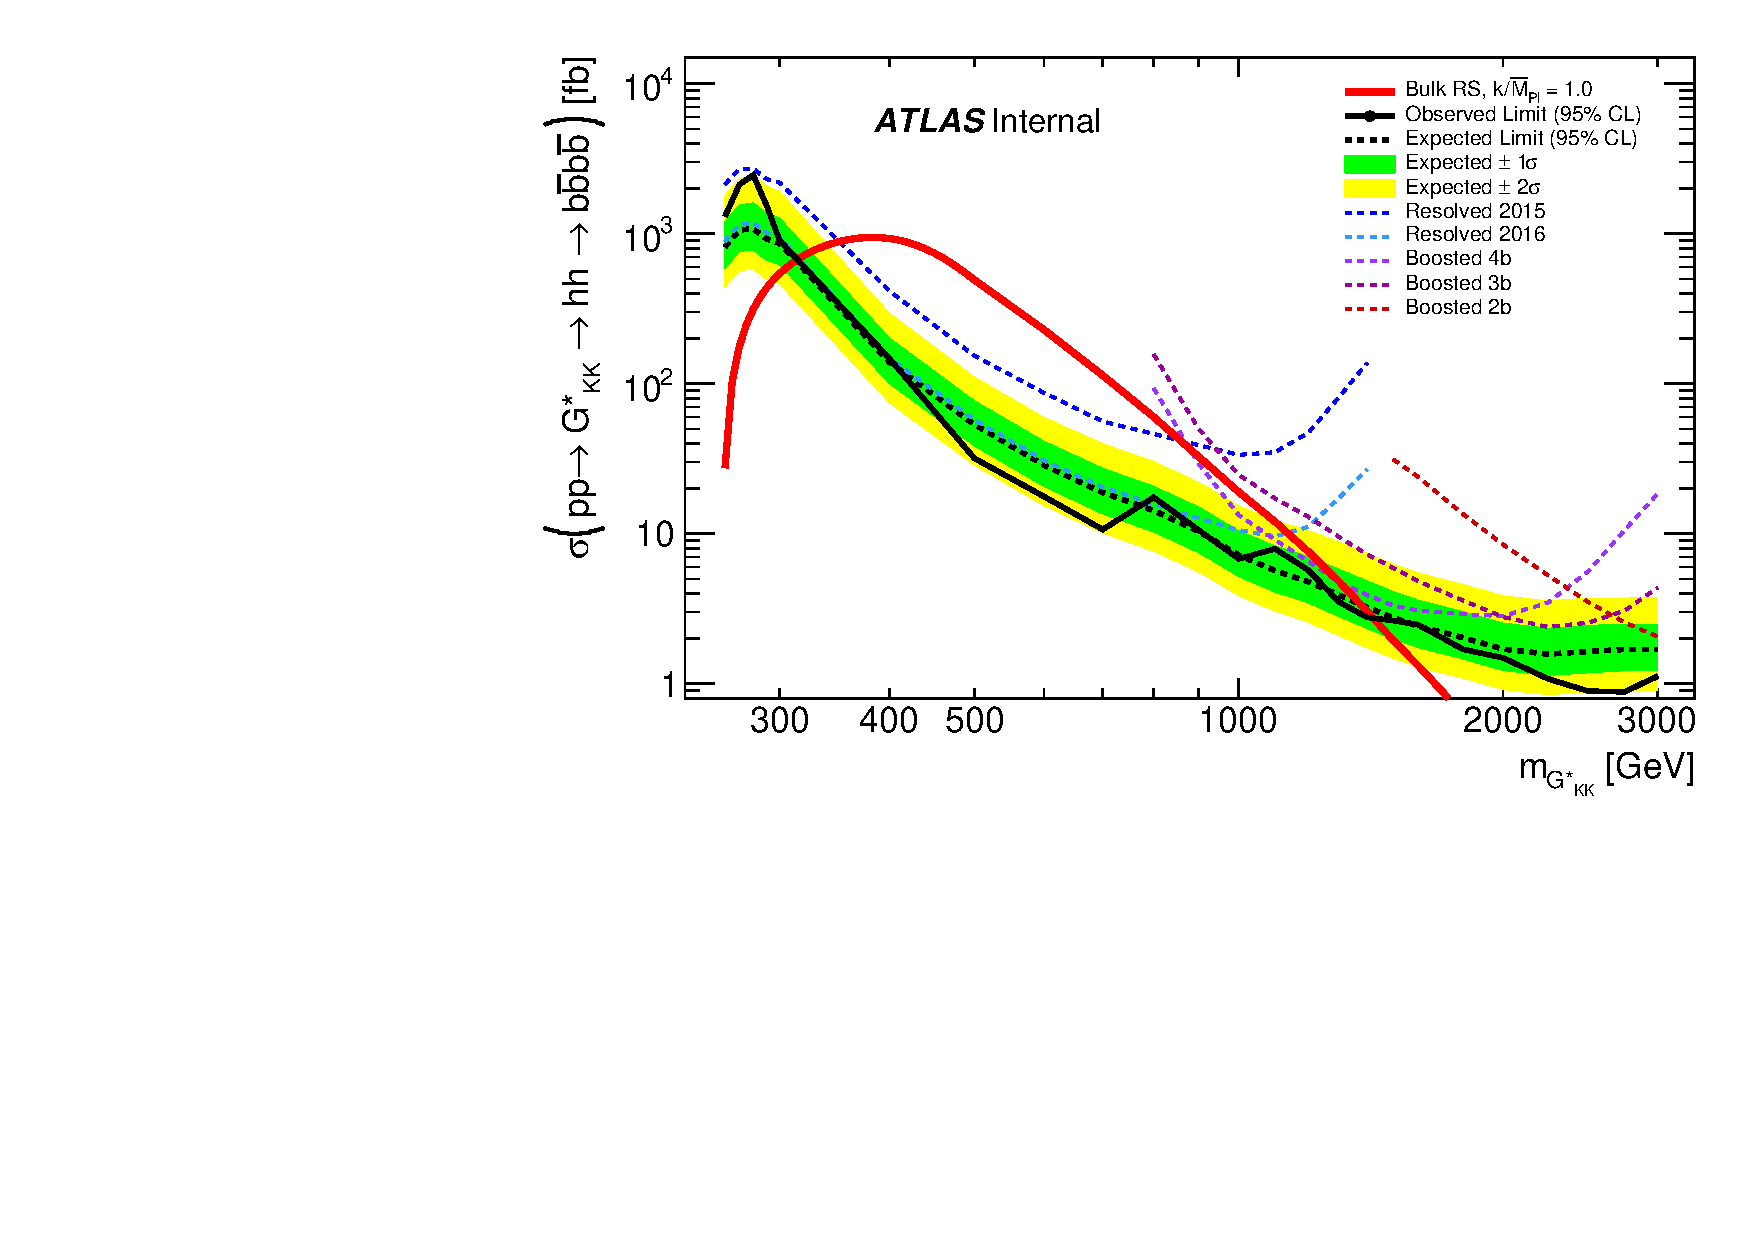
\includegraphics[width=0.4\textwidth,angle=-90]{figures/boosted/results/BrazilPlot_Asymptotic_g_hh_c10_combined_AllSyst_unblinded_2017-10-04.pdf}
\caption{The expected and observed $95\%$ CL upper exclusion limits for the combined analysis calculated including all systematic uncertainties for the $c=1.0$ \Grav. The dot-dashed line shows the expected limit when only statistical uncertainties are included. The limits are derived with the asymptotic approximation.}
\label{fig:limit_g20}
\end{center}
\end{figure*}

\begin{figure*}
\begin{center}
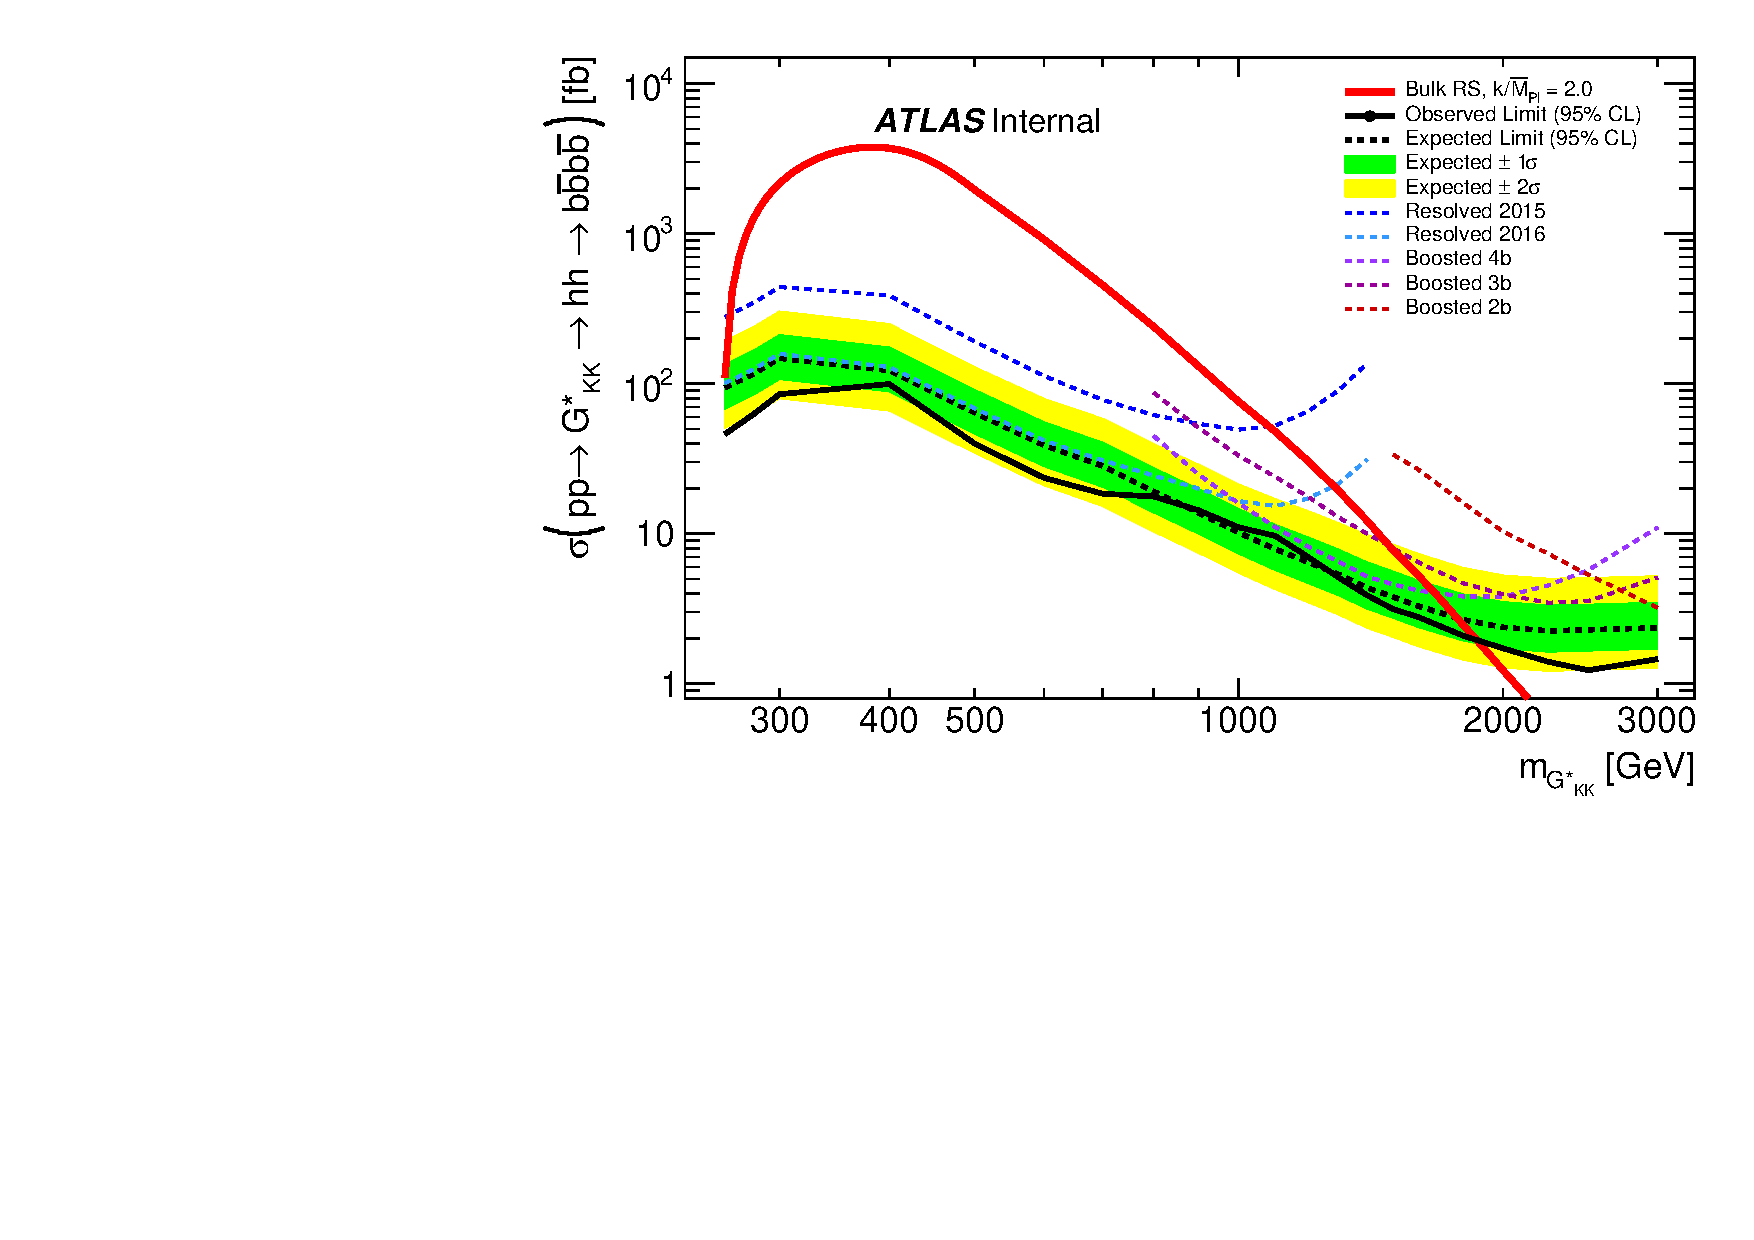
\includegraphics[width=0.4\textwidth,angle=-90]{figures/boosted/results/BrazilPlot_Asymptotic_g_hh_c20_combined_AllSyst_unblinded_2017-10-09.pdf}
\caption{The expected and observed $95\%$ CL upper exclusion limits for the combined analysis calculated including all systematic uncertainties for the $c=2.0$ \Grav. The dot-dashed line shows the expected limit when only statistical uncertainties are included. The limits are derived with the asymptotic approximation.}
\label{fig:limit_scalar}
\end{center}
\end{figure*}
